\documentclass[a4paper]{book}
\usepackage{a4wide}
\usepackage{makeidx}
\usepackage{graphicx}
\usepackage{multicol}
\usepackage{float}
\usepackage{listings}
\usepackage{color}
\usepackage{textcomp}
\usepackage{alltt}
\usepackage{times}
\usepackage{ifpdf}
\ifpdf
\usepackage[pdftex,
            pagebackref=true,
            colorlinks=true,
            linkcolor=blue,
            unicode
           ]{hyperref}
\else
\usepackage[ps2pdf,
            pagebackref=true,
            colorlinks=true,
            linkcolor=blue,
            unicode
           ]{hyperref}
\usepackage{pspicture}
\fi
\usepackage[utf8]{inputenc}
\usepackage{doxygen}
\lstset{language=C++,inputencoding=utf8,basicstyle=\footnotesize,breaklines=true,breakatwhitespace=true,tabsize=8,numbers=left }
\makeindex
\setcounter{tocdepth}{3}
\renewcommand{\footrulewidth}{0.4pt}
\begin{document}
\hypersetup{pageanchor=false}
\begin{titlepage}
\vspace*{7cm}
\begin{center}
{\Large Variant }\\
\vspace*{1cm}
{\large Generated by Doxygen 1.6.1}\\
\vspace*{0.5cm}
{\small Mon Jun 19 14:14:19 2017}\\
\end{center}
\end{titlepage}
\clearemptydoublepage
\pagenumbering{roman}
\tableofcontents
\clearemptydoublepage
\pagenumbering{arabic}
\hypersetup{pageanchor=true}
\chapter{Namespace Index}
\section{Namespace List}
Here is a list of all documented namespaces with brief descriptions:\begin{DoxyCompactList}
\item\contentsline{section}{\hyperlink{namespaceIO}{IO} (Namespace containing all input/output tools )}{\pageref{namespaceIO}}{}
\end{DoxyCompactList}

\chapter{Class Index}
\section{Class Hierarchy}
This inheritance list is sorted roughly, but not completely, alphabetically\+:\begin{DoxyCompactList}
\item \contentsline{section}{compare\+\_\+coords}{\pageref{structcompare__coords}}{}
\item \contentsline{section}{compare\+\_\+sddandcoords}{\pageref{structcompare__sddandcoords}}{}
\item \contentsline{section}{Console}{\pageref{classConsole}}{}
\item \contentsline{section}{Coord\+Converter}{\pageref{classCoordConverter}}{}
\item \contentsline{section}{Domain}{\pageref{classDomain}}{}
\item \contentsline{section}{Engine}{\pageref{classEngine}}{}
\begin{DoxyCompactList}
\item \contentsline{section}{Hydro4x1}{\pageref{classHydro4x1}}{}
\item \contentsline{section}{Hydro4x2}{\pageref{classHydro4x2}}{}
\item \contentsline{section}{Hydro8x1}{\pageref{classHydro8x1}}{}
\end{DoxyCompactList}
\item std\+:\+:exception\begin{DoxyCompactList}
\item \contentsline{section}{Exception}{\pageref{classException}}{}
\end{DoxyCompactList}
\item \contentsline{section}{Geometry}{\pageref{classGeometry}}{}
\item \contentsline{section}{Quantity$<$ T $>$}{\pageref{classQuantity}}{}
\item \contentsline{section}{Quantity$<$ real $>$}{\pageref{classQuantity}}{}
\item \contentsline{section}{S\+D\+Distributed}{\pageref{classSDDistributed}}{}
\item \contentsline{section}{Thread\+Pool}{\pageref{classThreadPool}}{}
\item \contentsline{section}{Timer}{\pageref{classTimer}}{}
\item \contentsline{section}{Time\+Stamp}{\pageref{classTimeStamp}}{}
\item std\+:\+:vector$<$ T $>$\begin{DoxyCompactList}
\item \contentsline{section}{S\+D\+Shared}{\pageref{classSDShared}}{}
\end{DoxyCompactList}
\item \contentsline{section}{Worker}{\pageref{classWorker}}{}
\end{DoxyCompactList}

\chapter{Class Index}
\section{Class List}
Here are the classes, structs, unions and interfaces with brief descriptions\+:\begin{DoxyCompactList}
\item\contentsline{section}{\mbox{\hyperlink{structcompare__coords}{compare\+\_\+coords}} }{\pageref{structcompare__coords}}{}
\item\contentsline{section}{\mbox{\hyperlink{structcompare__sddandcoords}{compare\+\_\+sddandcoords}} }{\pageref{structcompare__sddandcoords}}{}
\item\contentsline{section}{\mbox{\hyperlink{classConsole}{Console}} }{\pageref{classConsole}}{}
\item\contentsline{section}{\mbox{\hyperlink{classCoordConverter}{Coord\+Converter}} \\*Converts 2\+D-\/coordinates to memory index for given S\+DD size }{\pageref{classCoordConverter}}{}
\item\contentsline{section}{\mbox{\hyperlink{classDomain}{Domain}} \\*\mbox{\hyperlink{classDomain}{Domain}} on which a scheme is executed }{\pageref{classDomain}}{}
\item\contentsline{section}{\mbox{\hyperlink{classEngine}{Engine}} \\*Base class used to program a numerical scheme }{\pageref{classEngine}}{}
\item\contentsline{section}{\mbox{\hyperlink{classException}{Exception}} }{\pageref{classException}}{}
\item\contentsline{section}{\mbox{\hyperlink{classGeometry}{Geometry}} \\*Tool providing various splits of S\+D\+Ds (rectangular shapes) into S\+DS (any shape) }{\pageref{classGeometry}}{}
\item\contentsline{section}{\mbox{\hyperlink{classHydro4x1}{Hydro4x1}} \\*Donor-\/cell scheme for the Euler hydrodynamics equations }{\pageref{classHydro4x1}}{}
\item\contentsline{section}{\mbox{\hyperlink{classHydro4x2}{Hydro4x2}} \\*Donor-\/cell scheme for the Euler hydrodynamics equations }{\pageref{classHydro4x2}}{}
\item\contentsline{section}{\mbox{\hyperlink{classHydro8x1}{Hydro8x1}} \\*Donor-\/cell scheme for the Euler hydrodynamics equations }{\pageref{classHydro8x1}}{}
\item\contentsline{section}{\mbox{\hyperlink{classQuantity}{Quantity$<$ T $>$}} \\*Physical quantity used in numerical schemes }{\pageref{classQuantity}}{}
\item\contentsline{section}{\mbox{\hyperlink{classSDDistributed}{S\+D\+Distributed}} \\*Subdomain on distributed memory (S\+DD) }{\pageref{classSDDistributed}}{}
\item\contentsline{section}{\mbox{\hyperlink{classSDShared}{S\+D\+Shared}} \\*Subdomain on shared memory (S\+DS) }{\pageref{classSDShared}}{}
\item\contentsline{section}{\mbox{\hyperlink{classThreadPool}{Thread\+Pool}} }{\pageref{classThreadPool}}{}
\item\contentsline{section}{\mbox{\hyperlink{classTimer}{Timer}} }{\pageref{classTimer}}{}
\item\contentsline{section}{\mbox{\hyperlink{classTimeStamp}{Time\+Stamp}} }{\pageref{classTimeStamp}}{}
\item\contentsline{section}{\mbox{\hyperlink{classWorker}{Worker}} }{\pageref{classWorker}}{}
\end{DoxyCompactList}

\chapter{File Index}
\section{File List}
Here is a list of all documented files with brief descriptions\+:\begin{DoxyCompactList}
\item\contentsline{section}{source/engine/\hyperlink{source_2engine_2engine_8hpp}{engine.\+hpp} \\*Define the base \hyperlink{classEngine}{Engine} class for a numerical scheme }{\pageref{source_2engine_2engine_8hpp}}{}
\item\contentsline{section}{source/io/\hyperlink{source_2io_2IO_8hpp}{I\+O.\+hpp} \\*Input/\+Output tools }{\pageref{source_2io_2IO_8hpp}}{}
\item\contentsline{section}{source/project/conservative\+Hydrodynamics/\hyperlink{conservativeHydrodynamics_8hpp}{conservative\+Hydrodynamics.\+hpp} \\*Defines class of the upwind scheme for the hydrodynamics equations }{\pageref{conservativeHydrodynamics_8hpp}}{}
\item\contentsline{section}{source/project/donor\+Cell/{\bfseries donor\+Cell.\+hpp} }{\pageref{source_2project_2donorCell_2donorCell_8hpp}}{}
\item\contentsline{section}{source/project/hydrodynamics/\hyperlink{hydrodynamics_8hpp}{hydrodynamics.\+hpp} \\*Defines class of the upwind scheme for the hydrodynamics equations }{\pageref{hydrodynamics_8hpp}}{}
\item\contentsline{section}{source/project/isothermal\+Hydrodynamics/\hyperlink{isothermalHydrodynamics_8hpp}{isothermal\+Hydrodynamics.\+hpp} \\*Defines class of the upwind scheme for the hydrodynamics equations }{\pageref{isothermalHydrodynamics_8hpp}}{}
\item\contentsline{section}{source/project/transport\+Upwind/\hyperlink{source_2project_2transportUpwind_2transportUpwind_8hpp}{transport\+Upwind.\+hpp} \\*Defines class of the upwind scheme for the transport equation }{\pageref{source_2project_2transportUpwind_2transportUpwind_8hpp}}{}
\item\contentsline{section}{source/subdomain/\hyperlink{source_2subdomain_2CoordConverter_8hpp}{Coord\+Converter.\+hpp} \\*Defines class for the converter 2\+D-\/coordinates -\/$>$ memory index }{\pageref{source_2subdomain_2CoordConverter_8hpp}}{}
\item\contentsline{section}{source/subdomain/\hyperlink{source_2subdomain_2Domain_8hpp}{Domain.\+hpp} \\*Defines the \hyperlink{classDomain}{Domain} class }{\pageref{source_2subdomain_2Domain_8hpp}}{}
\item\contentsline{section}{source/subdomain/\hyperlink{source_2subdomain_2Geometry_8hpp}{Geometry.\+hpp} \\*Defines \hyperlink{classGeometry}{Geometry} class for S\+D\+Ss }{\pageref{source_2subdomain_2Geometry_8hpp}}{}
\item\contentsline{section}{source/subdomain/\hyperlink{source_2subdomain_2Quantity_8hpp}{Quantity.\+hpp} \\*Defines class for physical quantities used in a numerical scheme }{\pageref{source_2subdomain_2Quantity_8hpp}}{}
\item\contentsline{section}{source/subdomain/\hyperlink{source_2subdomain_2SDDistributed_8hpp}{S\+D\+Distributed.\+hpp} \\*Defines the class of subdomain on distributed memory (S\+DD) }{\pageref{source_2subdomain_2SDDistributed_8hpp}}{}
\item\contentsline{section}{source/subdomain/\hyperlink{source_2subdomain_2SDShared_8hpp}{S\+D\+Shared.\+hpp} \\*Defines class for subdomains on shared memory (S\+DS) }{\pageref{source_2subdomain_2SDShared_8hpp}}{}
\item\contentsline{section}{source/toolkit/exception/{\bfseries exception.\+hpp} }{\pageref{source_2toolkit_2exception_2exception_8hpp}}{}
\item\contentsline{section}{source/toolkit/number/{\bfseries number.\+hpp} }{\pageref{source_2toolkit_2number_2number_8hpp}}{}
\item\contentsline{section}{source/toolkit/threadpool/{\bfseries threadpool.\+hpp} }{\pageref{source_2toolkit_2threadpool_2threadpool_8hpp}}{}
\item\contentsline{section}{source/toolkit/timer/{\bfseries timer.\+hpp} }{\pageref{source_2toolkit_2timer_2timer_8hpp}}{}
\item\contentsline{section}{source/toolkit/timestamp/{\bfseries timestamp.\+h} }{\pageref{source_2toolkit_2timestamp_2timestamp_8h}}{}
\item\contentsline{section}{Variant/source/engine/\hyperlink{Variant_2source_2engine_2engine_8hpp}{engine.\+hpp} \\*Define the base \hyperlink{classEngine}{Engine} class for a numerical scheme }{\pageref{Variant_2source_2engine_2engine_8hpp}}{}
\item\contentsline{section}{Variant/source/io/\hyperlink{Variant_2source_2io_2IO_8hpp}{I\+O.\+hpp} \\*Input/\+Output tools }{\pageref{Variant_2source_2io_2IO_8hpp}}{}
\item\contentsline{section}{Variant/source/project/donor\+Cell/{\bfseries donor\+Cell.\+hpp} }{\pageref{Variant_2source_2project_2donorCell_2donorCell_8hpp}}{}
\item\contentsline{section}{Variant/source/project/transport\+Upwind/\hyperlink{Variant_2source_2project_2transportUpwind_2transportUpwind_8hpp}{transport\+Upwind.\+hpp} \\*Defines class of the upwind scheme for the transport equation }{\pageref{Variant_2source_2project_2transportUpwind_2transportUpwind_8hpp}}{}
\item\contentsline{section}{Variant/source/subdomain/\hyperlink{Variant_2source_2subdomain_2CoordConverter_8hpp}{Coord\+Converter.\+hpp} \\*Defines class for the converter 2\+D-\/coordinates -\/$>$ memory index }{\pageref{Variant_2source_2subdomain_2CoordConverter_8hpp}}{}
\item\contentsline{section}{Variant/source/subdomain/\hyperlink{Variant_2source_2subdomain_2Domain_8hpp}{Domain.\+hpp} \\*Defines the \hyperlink{classDomain}{Domain} class }{\pageref{Variant_2source_2subdomain_2Domain_8hpp}}{}
\item\contentsline{section}{Variant/source/subdomain/\hyperlink{Variant_2source_2subdomain_2Geometry_8hpp}{Geometry.\+hpp} \\*Defines \hyperlink{classGeometry}{Geometry} class for S\+D\+Ss }{\pageref{Variant_2source_2subdomain_2Geometry_8hpp}}{}
\item\contentsline{section}{Variant/source/subdomain/\hyperlink{Variant_2source_2subdomain_2Quantity_8hpp}{Quantity.\+hpp} \\*Defines class for physical quantities used in a numerical scheme }{\pageref{Variant_2source_2subdomain_2Quantity_8hpp}}{}
\item\contentsline{section}{Variant/source/subdomain/\hyperlink{Variant_2source_2subdomain_2SDDistributed_8hpp}{S\+D\+Distributed.\+hpp} \\*Defines the class of subdomain on distributed memory (S\+DD) }{\pageref{Variant_2source_2subdomain_2SDDistributed_8hpp}}{}
\item\contentsline{section}{Variant/source/subdomain/\hyperlink{Variant_2source_2subdomain_2SDShared_8hpp}{S\+D\+Shared.\+hpp} \\*Defines class for subdomains on shared memory (S\+DS) }{\pageref{Variant_2source_2subdomain_2SDShared_8hpp}}{}
\item\contentsline{section}{Variant/source/toolkit/exception/{\bfseries exception.\+hpp} }{\pageref{Variant_2source_2toolkit_2exception_2exception_8hpp}}{}
\item\contentsline{section}{Variant/source/toolkit/number/{\bfseries number.\+hpp} }{\pageref{Variant_2source_2toolkit_2number_2number_8hpp}}{}
\item\contentsline{section}{Variant/source/toolkit/threadpool/{\bfseries Thread\+Pool.\+h} }{\pageref{ThreadPool_8h}}{}
\item\contentsline{section}{Variant/source/toolkit/threadpool/{\bfseries threadpool.\+hpp} }{\pageref{Variant_2source_2toolkit_2threadpool_2threadpool_8hpp}}{}
\item\contentsline{section}{Variant/source/toolkit/timer/{\bfseries timer.\+hpp} }{\pageref{Variant_2source_2toolkit_2timer_2timer_8hpp}}{}
\item\contentsline{section}{Variant/source/toolkit/timestamp/{\bfseries timestamp.\+h} }{\pageref{Variant_2source_2toolkit_2timestamp_2timestamp_8h}}{}
\end{DoxyCompactList}

\chapter{Namespace Documentation}
\hypertarget{namespaceIO}{}\section{IO Namespace Reference}
\label{namespaceIO}\index{IO@{IO}}


Namespace containing all input/output tools.  


\subsection*{Functions}
\begin{DoxyCompactItemize}
\item 
int \mbox{\hyperlink{namespaceIO_ab1b5447a50be31c6e04b64a13c58a05d}{load\+Domain\+Info}} (std\+::string directory, \mbox{\hyperlink{classDomain}{Domain}} \&domain)
\begin{DoxyCompactList}\small\item\em Loads domain info and writes all necessary. \end{DoxyCompactList}\item 
int \mbox{\hyperlink{namespaceIO_acc60681d98975d0ce0d3580de4f70ecd}{load\+Scheme\+Info}} (std\+::string directory, \mbox{\hyperlink{classEngine}{Engine}} \&engine)
\begin{DoxyCompactList}\small\item\em Loads scheme info. \end{DoxyCompactList}\item 
int \mbox{\hyperlink{namespaceIO_ae9baa8f2d704798ba4b669718c5630c6}{load\+Exec\+Options}} (std\+::string directory, \mbox{\hyperlink{classDomain}{Domain}} \&domain)
\begin{DoxyCompactList}\small\item\em Loads execution options. \end{DoxyCompactList}\item 
int \mbox{\hyperlink{namespaceIO_a2d97d3a808e25f48fa483719b3927273}{load\+S\+D\+D\+Info}} (std\+::string directory, \mbox{\hyperlink{classDomain}{Domain}} \&domain)
\begin{DoxyCompactList}\small\item\em Loads characteristics of this node\textquotesingle{}s S\+DD. \end{DoxyCompactList}\item 
int \mbox{\hyperlink{namespaceIO_a0b5a994855e5e391320a431095d66400}{load\+Quantity}} (std\+::string directory, std\+::string quantity\+Name, \mbox{\hyperlink{classDomain}{Domain}} \&domain)
\begin{DoxyCompactList}\small\item\em Loads quantity data from file directory/quantity\+Name.\+dat. \end{DoxyCompactList}\item 
int \mbox{\hyperlink{namespaceIO_a7710f22e4bbbd375162154b69289e5e0}{load\+Boundary\+Conditions}} (std\+::string directory, \mbox{\hyperlink{classDomain}{Domain}} \&domain)
\begin{DoxyCompactList}\small\item\em Loads boundary conditions. \end{DoxyCompactList}\item 
int \mbox{\hyperlink{namespaceIO_a98f43edfc02e8c62ca9f005a9994ab69}{write\+Quantity}} (std\+::string directory, std\+::string quantity\+Name, const \mbox{\hyperlink{classDomain}{Domain}} \&domain)
\begin{DoxyCompactList}\small\item\em Writes quantity data into output file. \end{DoxyCompactList}\item 
\mbox{\Hypertarget{namespaceIO_aa44cb714db9cc88ac6497424ef0892e0}\label{namespaceIO_aa44cb714db9cc88ac6497424ef0892e0}} 
int {\bfseries write\+Perf\+Results} (std\+::string directory, const std\+::map$<$ std\+::string, int $>$ \&results)
\item 
\mbox{\Hypertarget{namespaceIO_a40ed72b5bd6bb86a441fe4e4722cf9eb}\label{namespaceIO_a40ed72b5bd6bb86a441fe4e4722cf9eb}} 
int {\bfseries write\+S\+D\+D\+Perf\+Results} (std\+::string directory, const \mbox{\hyperlink{classDomain}{Domain}} \&domain, const std\+::map$<$ std\+::string, int $>$ \&results)
\item 
\mbox{\Hypertarget{namespaceIO_a0f8d747d38ee614e50ace488d79ae520}\label{namespaceIO_a0f8d747d38ee614e50ace488d79ae520}} 
int {\bfseries write\+S\+D\+D\+Time} (std\+::string directory, const \mbox{\hyperlink{classDomain}{Domain}} \&domain, const std\+::string \&timer\+Name, const std\+::deque$<$ unsigned long int $>$ \&time\+Deque)
\item 
\mbox{\Hypertarget{namespaceIO_a9388e688bab072c402da7a19e5527ead}\label{namespaceIO_a9388e688bab072c402da7a19e5527ead}} 
int {\bfseries write\+Variant\+Info} (std\+::string directory, const \mbox{\hyperlink{classDomain}{Domain}} \&domain)
\end{DoxyCompactItemize}


\subsection{Detailed Description}
Namespace containing all input/output tools. 

\subsection{Function Documentation}
\mbox{\Hypertarget{namespaceIO_a7710f22e4bbbd375162154b69289e5e0}\label{namespaceIO_a7710f22e4bbbd375162154b69289e5e0}} 
\index{IO@{IO}!load\+Boundary\+Conditions@{load\+Boundary\+Conditions}}
\index{load\+Boundary\+Conditions@{load\+Boundary\+Conditions}!IO@{IO}}
\subsubsection{\texorpdfstring{load\+Boundary\+Conditions()}{loadBoundaryConditions()}}
{\footnotesize\ttfamily int I\+O\+::load\+Boundary\+Conditions (\begin{DoxyParamCaption}\item[{std\+::string}]{directory,  }\item[{\mbox{\hyperlink{classDomain}{Domain}} \&}]{domain }\end{DoxyParamCaption})}



Loads boundary conditions. 


\begin{DoxyParams}{Parameters}
{\em directory} & destination folder \\
\hline
{\em domain} & domain data \\
\hline
\end{DoxyParams}
\mbox{\Hypertarget{namespaceIO_ab1b5447a50be31c6e04b64a13c58a05d}\label{namespaceIO_ab1b5447a50be31c6e04b64a13c58a05d}} 
\index{IO@{IO}!load\+Domain\+Info@{load\+Domain\+Info}}
\index{load\+Domain\+Info@{load\+Domain\+Info}!IO@{IO}}
\subsubsection{\texorpdfstring{load\+Domain\+Info()}{loadDomainInfo()}}
{\footnotesize\ttfamily int I\+O\+::load\+Domain\+Info (\begin{DoxyParamCaption}\item[{std\+::string}]{directory,  }\item[{\mbox{\hyperlink{classDomain}{Domain}} \&}]{domain }\end{DoxyParamCaption})}



Loads domain info and writes all necessary. 

Data is written into file directory/domain.\+dat


\begin{DoxyParams}{Parameters}
{\em directory} & input folder \\
\hline
{\em domain} & domain to be updated with read data\\
\hline
\end{DoxyParams}
\begin{DoxyReturn}{Returns}
0 if loading succeeded, -\/1 otherwise 
\end{DoxyReturn}
\mbox{\Hypertarget{namespaceIO_ae9baa8f2d704798ba4b669718c5630c6}\label{namespaceIO_ae9baa8f2d704798ba4b669718c5630c6}} 
\index{IO@{IO}!load\+Exec\+Options@{load\+Exec\+Options}}
\index{load\+Exec\+Options@{load\+Exec\+Options}!IO@{IO}}
\subsubsection{\texorpdfstring{load\+Exec\+Options()}{loadExecOptions()}}
{\footnotesize\ttfamily int I\+O\+::load\+Exec\+Options (\begin{DoxyParamCaption}\item[{std\+::string}]{directory,  }\item[{\mbox{\hyperlink{classDomain}{Domain}} \&}]{domain }\end{DoxyParamCaption})}



Loads execution options. 

Loaded parameters are\+:
\begin{DoxyItemize}
\item number of S\+D\+Ds
\item number of S\+D\+Ss
\item S\+DS geometry
\end{DoxyItemize}


\begin{DoxyParams}{Parameters}
{\em directory} & input folder \\
\hline
{\em domain} & domain\\
\hline
\end{DoxyParams}
\begin{DoxyReturn}{Returns}
0 if loading succeeded, -\/1 otherwise 
\end{DoxyReturn}
\mbox{\Hypertarget{namespaceIO_a0b5a994855e5e391320a431095d66400}\label{namespaceIO_a0b5a994855e5e391320a431095d66400}} 
\index{IO@{IO}!load\+Quantity@{load\+Quantity}}
\index{load\+Quantity@{load\+Quantity}!IO@{IO}}
\subsubsection{\texorpdfstring{load\+Quantity()}{loadQuantity()}}
{\footnotesize\ttfamily int I\+O\+::load\+Quantity (\begin{DoxyParamCaption}\item[{std\+::string}]{directory,  }\item[{std\+::string}]{quantity\+Name,  }\item[{\mbox{\hyperlink{classDomain}{Domain}} \&}]{domain }\end{DoxyParamCaption})}



Loads quantity data from file directory/quantity\+Name.\+dat. 


\begin{DoxyParams}{Parameters}
{\em directory} & input folder \\
\hline
{\em quantity\+Name} & string name of quantity to be written \\
\hline
{\em domain} & domain \\
\hline
\end{DoxyParams}
\mbox{\Hypertarget{namespaceIO_acc60681d98975d0ce0d3580de4f70ecd}\label{namespaceIO_acc60681d98975d0ce0d3580de4f70ecd}} 
\index{IO@{IO}!load\+Scheme\+Info@{load\+Scheme\+Info}}
\index{load\+Scheme\+Info@{load\+Scheme\+Info}!IO@{IO}}
\subsubsection{\texorpdfstring{load\+Scheme\+Info()}{loadSchemeInfo()}}
{\footnotesize\ttfamily int I\+O\+::load\+Scheme\+Info (\begin{DoxyParamCaption}\item[{std\+::string}]{directory,  }\item[{\mbox{\hyperlink{classEngine}{Engine}} \&}]{engine }\end{DoxyParamCaption})}



Loads scheme info. 

Loaded parameters are\+:
\begin{DoxyItemize}
\item final time T
\item C\+FL condition
\end{DoxyItemize}


\begin{DoxyParams}{Parameters}
{\em directory} & input folder \\
\hline
{\em engine} & scheme engine\\
\hline
\end{DoxyParams}
\begin{DoxyReturn}{Returns}
0 if loading succeeded, -\/1 otherwise 
\end{DoxyReturn}
\mbox{\Hypertarget{namespaceIO_a2d97d3a808e25f48fa483719b3927273}\label{namespaceIO_a2d97d3a808e25f48fa483719b3927273}} 
\index{IO@{IO}!load\+S\+D\+D\+Info@{load\+S\+D\+D\+Info}}
\index{load\+S\+D\+D\+Info@{load\+S\+D\+D\+Info}!IO@{IO}}
\subsubsection{\texorpdfstring{load\+S\+D\+D\+Info()}{loadSDDInfo()}}
{\footnotesize\ttfamily int I\+O\+::load\+S\+D\+D\+Info (\begin{DoxyParamCaption}\item[{std\+::string}]{directory,  }\item[{\mbox{\hyperlink{classDomain}{Domain}} \&}]{domain }\end{DoxyParamCaption})}



Loads characteristics of this node\textquotesingle{}s S\+DD. 

Loaded parameters are\+:
\begin{DoxyItemize}
\item bottom-\/left coordinates of S\+DD on domain
\item width and height of S\+DD
\end{DoxyItemize}


\begin{DoxyParams}{Parameters}
{\em directory} & input folder \\
\hline
{\em domain} & domain \\
\hline
\end{DoxyParams}
\mbox{\Hypertarget{namespaceIO_a98f43edfc02e8c62ca9f005a9994ab69}\label{namespaceIO_a98f43edfc02e8c62ca9f005a9994ab69}} 
\index{IO@{IO}!write\+Quantity@{write\+Quantity}}
\index{write\+Quantity@{write\+Quantity}!IO@{IO}}
\subsubsection{\texorpdfstring{write\+Quantity()}{writeQuantity()}}
{\footnotesize\ttfamily int I\+O\+::write\+Quantity (\begin{DoxyParamCaption}\item[{std\+::string}]{directory,  }\item[{std\+::string}]{quantity\+Name,  }\item[{const \mbox{\hyperlink{classDomain}{Domain}} \&}]{domain }\end{DoxyParamCaption})}



Writes quantity data into output file. 


\begin{DoxyParams}{Parameters}
{\em directory} & destination folder \\
\hline
{\em quantity\+Name} & name of the quantity to output \\
\hline
{\em domain} & domain data\\
\hline
\end{DoxyParams}
\begin{DoxyReturn}{Returns}
0 if writing succeeded, -\/1 otherwise 
\end{DoxyReturn}

\chapter{Class Documentation}
\hypertarget{classConsole}{}\section{Console Class Reference}
\label{classConsole}\index{Console@{Console}}
\subsection*{Public Types}
\begin{DoxyCompactItemize}
\item 
\mbox{\Hypertarget{classConsole_af4999210d240ff9706a5a08a2fc7d80f}\label{classConsole_af4999210d240ff9706a5a08a2fc7d80f}} 
enum {\bfseries Mode} \{ \newline
{\bfseries \+\_\+normal}, 
{\bfseries \+\_\+bold}, 
{\bfseries \+\_\+black}, 
{\bfseries \+\_\+red}, 
\newline
{\bfseries \+\_\+green}, 
{\bfseries \+\_\+yellow}, 
{\bfseries \+\_\+blue}, 
{\bfseries \+\_\+pink}, 
\newline
{\bfseries \+\_\+cyan}
 \}
\end{DoxyCompactItemize}
\subsection*{Static Public Member Functions}
\begin{DoxyCompactItemize}
\item 
\mbox{\Hypertarget{classConsole_a1254fa9dfc22b645b18ff8beffb92ada}\label{classConsole_a1254fa9dfc22b645b18ff8beffb92ada}} 
static void {\bfseries color} (char c)
\item 
\mbox{\Hypertarget{classConsole_afc3a9b51e05728d4805421579a87f8c1}\label{classConsole_afc3a9b51e05728d4805421579a87f8c1}} 
static void {\bfseries bell} (int n)
\item 
\mbox{\Hypertarget{classConsole_a12fdea03e68fdec66289329fd34111c9}\label{classConsole_a12fdea03e68fdec66289329fd34111c9}} 
static void {\bfseries bold} ()
\item 
\mbox{\Hypertarget{classConsole_a2ec015ca344b10710aa5cf2ff578e9fe}\label{classConsole_a2ec015ca344b10710aa5cf2ff578e9fe}} 
static void {\bfseries clreol} ()
\item 
\mbox{\Hypertarget{classConsole_a24f860d3d5cb225b664c33b21f22cf8b}\label{classConsole_a24f860d3d5cb225b664c33b21f22cf8b}} 
static void {\bfseries clrscreen} ()
\item 
\mbox{\Hypertarget{classConsole_ac28051c7f6cd8f4bcaf0a8b8338cbaa9}\label{classConsole_ac28051c7f6cd8f4bcaf0a8b8338cbaa9}} 
static void {\bfseries cursoff} ()
\item 
\mbox{\Hypertarget{classConsole_accae861cddb51fde1c7a0000379270d1}\label{classConsole_accae861cddb51fde1c7a0000379270d1}} 
static void {\bfseries curson} ()
\item 
\mbox{\Hypertarget{classConsole_ac6353601b974fc3d40ab4d1b29052f00}\label{classConsole_ac6353601b974fc3d40ab4d1b29052f00}} 
static void {\bfseries home} ()
\item 
\mbox{\Hypertarget{classConsole_ab9f1622719fd6006b5f23a25dc148109}\label{classConsole_ab9f1622719fd6006b5f23a25dc148109}} 
static void {\bfseries insert} ()
\item 
\mbox{\Hypertarget{classConsole_a0af50381e547a4ad90b0fc5d82d3d9c0}\label{classConsole_a0af50381e547a4ad90b0fc5d82d3d9c0}} 
static void {\bfseries normal} ()
\item 
\mbox{\Hypertarget{classConsole_a00f6a2d90f6788226f7640fbdc399be9}\label{classConsole_a00f6a2d90f6788226f7640fbdc399be9}} 
static void {\bfseries poscur} (int l, int c)
\item 
\mbox{\Hypertarget{classConsole_a8bbc999f5c03ee649261f395113f3327}\label{classConsole_a8bbc999f5c03ee649261f395113f3327}} 
static void {\bfseries replace} ()
\item 
\mbox{\Hypertarget{classConsole_acdbffad9e6d5faf3654f2f662a885c05}\label{classConsole_acdbffad9e6d5faf3654f2f662a885c05}} 
static void {\bfseries underline} ()
\item 
\mbox{\Hypertarget{classConsole_a0c0b82ca8465e8d07d1c1000fd1c7065}\label{classConsole_a0c0b82ca8465e8d07d1c1000fd1c7065}} 
static void {\bfseries videoff} ()
\item 
\mbox{\Hypertarget{classConsole_a9452e745b8255bfc5c01914e284a6dde}\label{classConsole_a9452e745b8255bfc5c01914e284a6dde}} 
static void {\bfseries videon} ()
\item 
\mbox{\Hypertarget{classConsole_a0d4128ee5041ea69f58cbb0d200a2f80}\label{classConsole_a0d4128ee5041ea69f58cbb0d200a2f80}} 
static void {\bfseries blink} ()
\end{DoxyCompactItemize}
\subsection*{Static Public Attributes}
\begin{DoxyCompactItemize}
\item 
\mbox{\Hypertarget{classConsole_abf80bf3470dade29c45fed14ee6e9d38}\label{classConsole_abf80bf3470dade29c45fed14ee6e9d38}} 
static const int {\bfseries esc} = 27
\end{DoxyCompactItemize}
\subsection*{Friends}
\begin{DoxyCompactItemize}
\item 
\mbox{\Hypertarget{classConsole_aff1b0921f7ab18e456bfb58711afdaea}\label{classConsole_aff1b0921f7ab18e456bfb58711afdaea}} 
std\+::ostream \& {\bfseries operator$<$$<$} (std\+::ostream \&os, const Mode \&mode)
\end{DoxyCompactItemize}


The documentation for this class was generated from the following file\+:\begin{DoxyCompactItemize}
\item 
source/toolkit/exception/exception.\+hpp\end{DoxyCompactItemize}

\hypertarget{classCoordConverter}{}\section{Coord\+Converter Class Reference}
\label{classCoordConverter}\index{Coord\+Converter@{Coord\+Converter}}


Converts 2\+D-\/coordinates to memory index for given S\+DD size.  




{\ttfamily \#include $<$Coord\+Converter.\+hpp$>$}

\subsection*{Public Member Functions}
\begin{DoxyCompactItemize}
\item 
\hyperlink{classCoordConverter_a0e773a3ee5461119d7ff285fde45427d}{Coord\+Converter} (unsigned int size\+S\+D\+D\+\_\+X, unsigned int size\+S\+D\+D\+\_\+Y, unsigned int boundary\+Thickness)
\begin{DoxyCompactList}\small\item\em Constructor. \end{DoxyCompactList}\item 
\hyperlink{classCoordConverter_af11209a489a46dd335db0635d811999d}{Coord\+Converter} (const \hyperlink{classCoordConverter}{Coord\+Converter} \&coord\+Converter)
\begin{DoxyCompactList}\small\item\em Copy constructor. \end{DoxyCompactList}\item 
\mbox{\Hypertarget{classCoordConverter_ae62fc899a25ed7b6455927a6ddcccf52}\label{classCoordConverter_ae62fc899a25ed7b6455927a6ddcccf52}} 
unsigned int \hyperlink{classCoordConverter_ae62fc899a25ed7b6455927a6ddcccf52}{convert} (int coordX, int coordY) const
\begin{DoxyCompactList}\small\item\em convert 2\+D-\/coordinates to the memory index of the data on the S\+DD \end{DoxyCompactList}\item 
\hyperlink{classCoordConverter_a0e773a3ee5461119d7ff285fde45427d}{Coord\+Converter} (unsigned int size\+S\+D\+D\+\_\+X, unsigned int size\+S\+D\+D\+\_\+Y, unsigned int boundary\+Thickness)
\begin{DoxyCompactList}\small\item\em Constructor. \end{DoxyCompactList}\item 
\hyperlink{classCoordConverter_af11209a489a46dd335db0635d811999d}{Coord\+Converter} (const \hyperlink{classCoordConverter}{Coord\+Converter} \&coord\+Converter)
\begin{DoxyCompactList}\small\item\em Copy constructor. \end{DoxyCompactList}\item 
\mbox{\Hypertarget{classCoordConverter_ae62fc899a25ed7b6455927a6ddcccf52}\label{classCoordConverter_ae62fc899a25ed7b6455927a6ddcccf52}} 
unsigned int \hyperlink{classCoordConverter_ae62fc899a25ed7b6455927a6ddcccf52}{convert} (int coordX, int coordY) const
\begin{DoxyCompactList}\small\item\em convert 2\+D-\/coordinates to the memory index of the data on the S\+DD \end{DoxyCompactList}\end{DoxyCompactItemize}


\subsection{Detailed Description}
Converts 2\+D-\/coordinates to memory index for given S\+DD size. 

The data on the S\+DD is stored as a one-\/dimensional array, hence the need of a converter. 

\subsection{Constructor \& Destructor Documentation}
\mbox{\Hypertarget{classCoordConverter_a0e773a3ee5461119d7ff285fde45427d}\label{classCoordConverter_a0e773a3ee5461119d7ff285fde45427d}} 
\index{Coord\+Converter@{Coord\+Converter}!Coord\+Converter@{Coord\+Converter}}
\index{Coord\+Converter@{Coord\+Converter}!Coord\+Converter@{Coord\+Converter}}
\subsubsection{\texorpdfstring{Coord\+Converter()}{CoordConverter()}\hspace{0.1cm}{\footnotesize\ttfamily [1/4]}}
{\footnotesize\ttfamily Coord\+Converter\+::\+Coord\+Converter (\begin{DoxyParamCaption}\item[{unsigned int}]{size\+S\+D\+D\+\_\+X,  }\item[{unsigned int}]{size\+S\+D\+D\+\_\+Y,  }\item[{unsigned int}]{boundary\+Thickness }\end{DoxyParamCaption})}



Constructor. 


\begin{DoxyParams}{Parameters}
{\em size\+S\+D\+D\+\_\+X} & \+: width of S\+DD \\
\hline
{\em size\+S\+D\+D\+\_\+Y} & \+: height of S\+DD \\
\hline
\end{DoxyParams}
\mbox{\Hypertarget{classCoordConverter_af11209a489a46dd335db0635d811999d}\label{classCoordConverter_af11209a489a46dd335db0635d811999d}} 
\index{Coord\+Converter@{Coord\+Converter}!Coord\+Converter@{Coord\+Converter}}
\index{Coord\+Converter@{Coord\+Converter}!Coord\+Converter@{Coord\+Converter}}
\subsubsection{\texorpdfstring{Coord\+Converter()}{CoordConverter()}\hspace{0.1cm}{\footnotesize\ttfamily [2/4]}}
{\footnotesize\ttfamily Coord\+Converter\+::\+Coord\+Converter (\begin{DoxyParamCaption}\item[{const \hyperlink{classCoordConverter}{Coord\+Converter} \&}]{coord\+Converter }\end{DoxyParamCaption})}



Copy constructor. 


\begin{DoxyParams}{Parameters}
{\em coord\+Converter} & \+: coordinates converter to copy \\
\hline
\end{DoxyParams}
\mbox{\Hypertarget{classCoordConverter_a0e773a3ee5461119d7ff285fde45427d}\label{classCoordConverter_a0e773a3ee5461119d7ff285fde45427d}} 
\index{Coord\+Converter@{Coord\+Converter}!Coord\+Converter@{Coord\+Converter}}
\index{Coord\+Converter@{Coord\+Converter}!Coord\+Converter@{Coord\+Converter}}
\subsubsection{\texorpdfstring{Coord\+Converter()}{CoordConverter()}\hspace{0.1cm}{\footnotesize\ttfamily [3/4]}}
{\footnotesize\ttfamily Coord\+Converter\+::\+Coord\+Converter (\begin{DoxyParamCaption}\item[{unsigned int}]{size\+S\+D\+D\+\_\+X,  }\item[{unsigned int}]{size\+S\+D\+D\+\_\+Y,  }\item[{unsigned int}]{boundary\+Thickness }\end{DoxyParamCaption})}



Constructor. 


\begin{DoxyParams}{Parameters}
{\em size\+S\+D\+D\+\_\+X} & \+: width of S\+DD \\
\hline
{\em size\+S\+D\+D\+\_\+Y} & \+: height of S\+DD \\
\hline
\end{DoxyParams}
\mbox{\Hypertarget{classCoordConverter_af11209a489a46dd335db0635d811999d}\label{classCoordConverter_af11209a489a46dd335db0635d811999d}} 
\index{Coord\+Converter@{Coord\+Converter}!Coord\+Converter@{Coord\+Converter}}
\index{Coord\+Converter@{Coord\+Converter}!Coord\+Converter@{Coord\+Converter}}
\subsubsection{\texorpdfstring{Coord\+Converter()}{CoordConverter()}\hspace{0.1cm}{\footnotesize\ttfamily [4/4]}}
{\footnotesize\ttfamily Coord\+Converter\+::\+Coord\+Converter (\begin{DoxyParamCaption}\item[{const \hyperlink{classCoordConverter}{Coord\+Converter} \&}]{coord\+Converter }\end{DoxyParamCaption})}



Copy constructor. 


\begin{DoxyParams}{Parameters}
{\em coord\+Converter} & \+: coordinates converter to copy \\
\hline
\end{DoxyParams}


The documentation for this class was generated from the following files\+:\begin{DoxyCompactItemize}
\item 
source/subdomain/\hyperlink{source_2subdomain_2CoordConverter_8hpp}{Coord\+Converter.\+hpp}\item 
source/subdomain/Coord\+Converter.\+cpp\end{DoxyCompactItemize}

\hypertarget{classDomain}{}\section{Domain Class Reference}
\label{classDomain}\index{Domain@{Domain}}


\hyperlink{classDomain}{Domain} on which a scheme is executed.  




{\ttfamily \#include $<$Domain.\+hpp$>$}

\subsection*{Public Member Functions}
\begin{DoxyCompactItemize}
\item 
\mbox{\Hypertarget{classDomain_a6adccae537e53d4fde2b70f875e6b8d0}\label{classDomain_a6adccae537e53d4fde2b70f875e6b8d0}} 
\hyperlink{classDomain_a6adccae537e53d4fde2b70f875e6b8d0}{Domain} ()
\begin{DoxyCompactList}\small\item\em Constructor. \end{DoxyCompactList}\item 
\mbox{\Hypertarget{classDomain_a29cec9afb2e54c810ba1f3c1a49543a8}\label{classDomain_a29cec9afb2e54c810ba1f3c1a49543a8}} 
\hyperlink{classDomain_a29cec9afb2e54c810ba1f3c1a49543a8}{$\sim$\+Domain} ()
\begin{DoxyCompactList}\small\item\em Destructor. \end{DoxyCompactList}\item 
void \hyperlink{classDomain_a853266061b629ff1f920b46c06c478d6}{init\+Rect} (real lx, real ly, unsigned int Nx, unsigned int Ny)
\begin{DoxyCompactList}\small\item\em Initializes domain rectangle. \end{DoxyCompactList}\item 
void \hyperlink{classDomain_a10a5e8384b21bb3c968699c2a6c89bf7}{set\+Options} (unsigned int n\+S\+DD, unsigned int n\+S\+D\+D\+\_\+X, unsigned int n\+S\+D\+D\+\_\+Y, unsigned int n\+S\+DS, std\+::string S\+D\+Sgeom, unsigned int n\+Threads)
\begin{DoxyCompactList}\small\item\em Changes options for building S\+D\+Ds and S\+D\+Ss. \end{DoxyCompactList}\item 
real \hyperlink{classDomain_a510afad91fe81eb2ccef203a980f4223}{getlx} () const
\begin{DoxyCompactList}\small\item\em Returns the non-\/modifiable width of the domain. \end{DoxyCompactList}\item 
real \hyperlink{classDomain_ac9cedab179bb0611fc0e9fcfbcedb835}{getly} () const
\begin{DoxyCompactList}\small\item\em Returns the non-\/modifiable height of the domain. \end{DoxyCompactList}\item 
unsigned int \hyperlink{classDomain_a75f299e3871fe9cec01637b140429ef9}{get\+SizeX} () const
\begin{DoxyCompactList}\small\item\em Returns the non-\/modifiable number of cells on the x-\/axis. \end{DoxyCompactList}\item 
unsigned int \hyperlink{classDomain_a66692b4f23353c9b1fe884e583770cb3}{get\+SizeY} () const
\begin{DoxyCompactList}\small\item\em Returns the non-\/modifiable number of cells on the y-\/axis. \end{DoxyCompactList}\item 
real \hyperlink{classDomain_acdb586f6ef994a1621680ec9b946aeb4}{getdx} () const
\begin{DoxyCompactList}\small\item\em Returns the non-\/modifiable space step on the x-\/axis (ie. the width of a cell). \end{DoxyCompactList}\item 
real \hyperlink{classDomain_a5e62ab8a8b53f67cc3c30b6066b10aac}{getdy} () const
\begin{DoxyCompactList}\small\item\em Returns the non-\/modifiable space step on the y-\/axis (ie. the height of a cell). \end{DoxyCompactList}\item 
\mbox{\Hypertarget{classDomain_a978917d5bf263dd1345f1a41c9edf661}\label{classDomain_a978917d5bf263dd1345f1a41c9edf661}} 
unsigned int {\bfseries get\+Number\+S\+DD} () const
\item 
\mbox{\Hypertarget{classDomain_a02cc51cc2e5d976810039e7118382cde}\label{classDomain_a02cc51cc2e5d976810039e7118382cde}} 
unsigned int {\bfseries get\+Number\+S\+D\+D\+\_\+X} () const
\item 
\mbox{\Hypertarget{classDomain_a8e8d6c959123597f6e2d8779a836d32c}\label{classDomain_a8e8d6c959123597f6e2d8779a836d32c}} 
unsigned int {\bfseries get\+Number\+S\+D\+D\+\_\+Y} () const
\item 
\mbox{\Hypertarget{classDomain_a985c94d1108a0a206f0201908d944a0d}\label{classDomain_a985c94d1108a0a206f0201908d944a0d}} 
unsigned int {\bfseries get\+Number\+Neighbour\+S\+D\+Ds} () const
\item 
\mbox{\Hypertarget{classDomain_a428011ce5e842c9f05545c57480ed30e}\label{classDomain_a428011ce5e842c9f05545c57480ed30e}} 
unsigned int {\bfseries get\+Number\+Physical\+Cells} () const
\item 
\mbox{\Hypertarget{classDomain_adbbd89acedd87b8b4814e367027551cd}\label{classDomain_adbbd89acedd87b8b4814e367027551cd}} 
unsigned int {\bfseries get\+Number\+Overlap\+Cells} () const
\item 
\mbox{\Hypertarget{classDomain_ab3a77c402326dc31a855125536348a6f}\label{classDomain_ab3a77c402326dc31a855125536348a6f}} 
unsigned int {\bfseries get\+Number\+Boundary\+Cells} () const
\item 
\mbox{\Hypertarget{classDomain_a25e60a79720035ab95a1eb4a41efb53c}\label{classDomain_a25e60a79720035ab95a1eb4a41efb53c}} 
unsigned int {\bfseries get\+Number\+S\+DS} () const
\item 
\mbox{\Hypertarget{classDomain_a388103cf2adcc7224f77d4c26a471d6a}\label{classDomain_a388103cf2adcc7224f77d4c26a471d6a}} 
std\+::string {\bfseries get\+S\+D\+S\+Geometry} () const
\item 
\mbox{\Hypertarget{classDomain_ac1e1ec57c7c0401dbee987d1c760ced7}\label{classDomain_ac1e1ec57c7c0401dbee987d1c760ced7}} 
unsigned int {\bfseries get\+Number\+Threads} () const
\item 
std\+::vector$<$ unsigned int $>$ \hyperlink{classDomain_a6f7d5f16ca53367feabc00b9efa05be8}{get\+Uid\+List} () const
\begin{DoxyCompactList}\small\item\em Returns vector containing unique ids of all cells. \end{DoxyCompactList}\item 
unsigned int \hyperlink{classDomain_aa0d225e23c6a454058a3df5b7b5973fa}{get\+Boundary\+Thickness} ()
\begin{DoxyCompactList}\small\item\em Returns boundary thickness of the domain, ie. the number of layers of cells outside the computed domain. \end{DoxyCompactList}\item 
std\+::pair$<$ int, int $>$ \hyperlink{classDomain_a29e2005bed3aa17f036b8d2b36084153}{get\+B\+L\+Of\+S\+DD} (unsigned int S\+D\+Did) const
\begin{DoxyCompactList}\small\item\em Gets bottom-\/left coordinates of S\+DD given by its id. \end{DoxyCompactList}\item 
std\+::pair$<$ int, int $>$ \hyperlink{classDomain_a1d2f7ee9336c682d4d6b01893d0beb4f}{get\+Coords\+On\+Domain} (unsigned int uid) const
\begin{DoxyCompactList}\small\item\em Gets coordinates on computed domain of cell given by its unique id. \end{DoxyCompactList}\item 
std\+::pair$<$ char, real $>$ \hyperlink{classDomain_a1f219d1f46645da98f538dada37432f9}{get\+Boundary\+Condition} (std\+::pair$<$ int, int $>$ coords\+On\+S\+DD) const
\begin{DoxyCompactList}\small\item\em Returns boundary condition on a cell given by its coordinates on the domain. \end{DoxyCompactList}\item 
\mbox{\Hypertarget{classDomain_a657f0b6750e14d1d3cde6afd8b1e9b48}\label{classDomain_a657f0b6750e14d1d3cde6afd8b1e9b48}} 
unsigned int \hyperlink{classDomain_a657f0b6750e14d1d3cde6afd8b1e9b48}{get\+Uid} (std\+::pair$<$ int, int $>$ coords\+On\+Domain) const
\begin{DoxyCompactList}\small\item\em Returns non-\/modifiable unique id of cell given by its coordinates on the domain. \end{DoxyCompactList}\item 
\mbox{\Hypertarget{classDomain_a677ba729e74d00b167b51ab6c921782a}\label{classDomain_a677ba729e74d00b167b51ab6c921782a}} 
int \hyperlink{classDomain_a677ba729e74d00b167b51ab6c921782a}{get\+Boundary\+Side} (std\+::pair$<$ int, int $>$ coords) const
\begin{DoxyCompactList}\small\item\em Returns boundary side (left, right, top, bottom or inside if not on boundary) of a cell given by its coordinates on the domain. \end{DoxyCompactList}\item 
void \hyperlink{classDomain_a1463e043dbcda6e6755dda83c26d6b73}{add\+Coord} (unsigned int uid, std\+::pair$<$ int, int $>$ coords)
\begin{DoxyCompactList}\small\item\em Adds new unique id $<$-\/$>$ coords on domain correspondence on a given cell. \end{DoxyCompactList}\item 
void \hyperlink{classDomain_a139f4270151467a3380922e98c644f79}{add\+Boundary\+Coords} (unsigned int uid, std\+::pair$<$ int, int $>$ coords, char B\+Ctype, real value)
\begin{DoxyCompactList}\small\item\em Adds new unique id $<$-\/$>$ coords on domain correspondenc\+Pieśnie and boundary condition for a cell on the boundary. \end{DoxyCompactList}\item 
void \hyperlink{classDomain_a4bad9ce1ce7d7fc7ef5b564bd5ac21e1}{add\+Quantity} (std\+::string quantity\+Name, bool constant=false)
\begin{DoxyCompactList}\small\item\em Adds new quantity to be managed by the scheme. \end{DoxyCompactList}\item 
void \hyperlink{classDomain_a3be46362fe91960104764d9eb89f1d29}{add\+Equation} (std\+::string eq\+Name, eq\+Type eq\+Func)
\begin{DoxyCompactList}\small\item\em Adds function that resolves a new equation on a S\+DS to be computed for each iteration by the domain. \end{DoxyCompactList}\item 
void \hyperlink{classDomain_af1262b85d13fbbf90388e453d9602372}{build\+Sub\+Domains\+M\+PI} ()
\begin{DoxyCompactList}\small\item\em Builds subdomains according to set options. \end{DoxyCompactList}\item 
\mbox{\Hypertarget{classDomain_a4d1ecd27481f6c7c0b077225fa48bc99}\label{classDomain_a4d1ecd27481f6c7c0b077225fa48bc99}} 
void \hyperlink{classDomain_a4d1ecd27481f6c7c0b077225fa48bc99}{build\+Boundary\+Map} ()
\begin{DoxyCompactList}\small\item\em Builds all info needed by the domain to compute the boundary according to the boundary conditions set on boundary cells. \end{DoxyCompactList}\item 
void \hyperlink{classDomain_aa2e6cebf44a57323f3c6344d131126c1}{build\+Threads} ()
\begin{DoxyCompactList}\small\item\em Builds the task pool for each S\+DD. \end{DoxyCompactList}\item 
\mbox{\Hypertarget{classDomain_a25f3b3d25cb0a864f0c3e380cb9044be}\label{classDomain_a25f3b3d25cb0a864f0c3e380cb9044be}} 
void \hyperlink{classDomain_a25f3b3d25cb0a864f0c3e380cb9044be}{exec\+Equation} (std\+::string eq\+Name)
\begin{DoxyCompactList}\small\item\em Calls all added equations, ie. computes an iteration of the scheme on the domain. \end{DoxyCompactList}\item 
void \hyperlink{classDomain_a4411f8eb6c118c84f16d62a411b4432a}{update\+Overlap\+Cells} ()
\begin{DoxyCompactList}\small\item\em updates overlap cells of all S\+D\+Ds according to their values on reference cells on other S\+D\+Ds, for a given quantity. \end{DoxyCompactList}\item 
\mbox{\Hypertarget{classDomain_a3e6670e39e3a6265ee57baeb70aa8867}\label{classDomain_a3e6670e39e3a6265ee57baeb70aa8867}} 
void {\bfseries update\+Overlap\+Cells} (std\+::string qty\+Name)
\item 
void \hyperlink{classDomain_af169473470489edc4235399887c10da0}{update\+Boundary\+Cells} (std\+::string quantity\+Name, bool change\+Neumann\+To\+Opposite=false)
\begin{DoxyCompactList}\small\item\em updates boundary of all S\+D\+Ds according to their values on reference cells on other S\+D\+Ds, for a given quantity. \end{DoxyCompactList}\item 
std\+::pair$<$ int, std\+::pair$<$ int, int $>$ $>$ \hyperlink{classDomain_a5b3fd7cbe29576ea63219b326c15680e}{get\+S\+D\+Dand\+Coords} (std\+::pair$<$ int, int $>$ coords\+On\+Domain) const
\begin{DoxyCompactList}\small\item\em Returns non-\/modifiable id of S\+DD and coordinates on S\+DD of cell given by its coordinates on the domain. \end{DoxyCompactList}\item 
std\+::pair$<$ int, std\+::pair$<$ int, int $>$ $>$ \hyperlink{classDomain_af6442039d5c64b9a59b7a1bd94fc6bbb}{get\+S\+D\+Dand\+Coords} (unsigned int S\+D\+Did, std\+::pair$<$ int, int $>$ coords) const
\begin{DoxyCompactList}\small\item\em Returns non-\/modifiable id of S\+DD and coordinates on S\+DD of cell given by its coordinates on the domain. \end{DoxyCompactList}\item 
void \hyperlink{classDomain_a1163559d75540c4cd29c7aa775feca80}{print\+State} (std\+::string quantity\+Name)
\begin{DoxyCompactList}\small\item\em Prints quantity values for all cells. \end{DoxyCompactList}\item 
void \hyperlink{classDomain_acc1225a3c5e6e2a808c88d187adc7d3c}{set\+S\+D\+D\+Info} (unsigned int B\+L\+\_\+X, unsigned int B\+L\+\_\+Y, unsigned int Nx, unsigned int Ny)
\begin{DoxyCompactList}\small\item\em Change characteristics of S\+DD (bottom-\/left and size) \end{DoxyCompactList}\item 
\hyperlink{classSDDistributed}{S\+D\+Distributed} \& \hyperlink{classDomain_a26ceb37145bc70b3cc85e15e24a54287}{get\+S\+DD} ()
\begin{DoxyCompactList}\small\item\em Returns reference to S\+DD possessed by this M\+PI node. \end{DoxyCompactList}\item 
const \hyperlink{classSDDistributed}{S\+D\+Distributed} \& \hyperlink{classDomain_a8172470afa3d3ec4c7202c8ee25ab3b8}{get\+S\+D\+Dconst} () const
\begin{DoxyCompactList}\small\item\em Returns const reference to S\+DD possessed by this M\+PI node. \end{DoxyCompactList}\item 
\mbox{\Hypertarget{classDomain_a9f12ce216ba0fdb5e46147875f9a97a3}\label{classDomain_a9f12ce216ba0fdb5e46147875f9a97a3}} 
void {\bfseries switch\+Quantity\+Prev\+Next} (std\+::string quantity\+Name)
\item 
\mbox{\Hypertarget{classDomain_a6adccae537e53d4fde2b70f875e6b8d0}\label{classDomain_a6adccae537e53d4fde2b70f875e6b8d0}} 
\hyperlink{classDomain_a6adccae537e53d4fde2b70f875e6b8d0}{Domain} ()
\begin{DoxyCompactList}\small\item\em Constructor. \end{DoxyCompactList}\item 
\mbox{\Hypertarget{classDomain_a29cec9afb2e54c810ba1f3c1a49543a8}\label{classDomain_a29cec9afb2e54c810ba1f3c1a49543a8}} 
\hyperlink{classDomain_a29cec9afb2e54c810ba1f3c1a49543a8}{$\sim$\+Domain} ()
\begin{DoxyCompactList}\small\item\em Destructor. \end{DoxyCompactList}\item 
void \hyperlink{classDomain_a853266061b629ff1f920b46c06c478d6}{init\+Rect} (real lx, real ly, unsigned int Nx, unsigned int Ny)
\begin{DoxyCompactList}\small\item\em Initializes domain rectangle. \end{DoxyCompactList}\item 
void \hyperlink{classDomain_a10a5e8384b21bb3c968699c2a6c89bf7}{set\+Options} (unsigned int n\+S\+DD, unsigned int n\+S\+D\+D\+\_\+X, unsigned int n\+S\+D\+D\+\_\+Y, unsigned int n\+S\+DS, std\+::string S\+D\+Sgeom, unsigned int n\+Threads)
\begin{DoxyCompactList}\small\item\em Changes options for building S\+D\+Ds and S\+D\+Ss. \end{DoxyCompactList}\item 
std\+::vector$<$ \hyperlink{classSDDistributed}{S\+D\+Distributed} $\ast$ $>$ \hyperlink{classDomain_ae560ad14f723c01663bbb783ede30fd8}{get\+S\+DD} () const
\begin{DoxyCompactList}\small\item\em Returns vector of pointers to S\+D\+Ds of the domain. \end{DoxyCompactList}\item 
real \hyperlink{classDomain_a510afad91fe81eb2ccef203a980f4223}{getlx} () const
\begin{DoxyCompactList}\small\item\em Returns the non-\/modifiable width of the domain. \end{DoxyCompactList}\item 
real \hyperlink{classDomain_ac9cedab179bb0611fc0e9fcfbcedb835}{getly} () const
\begin{DoxyCompactList}\small\item\em Returns the non-\/modifiable height of the domain. \end{DoxyCompactList}\item 
unsigned int \hyperlink{classDomain_a75f299e3871fe9cec01637b140429ef9}{get\+SizeX} () const
\begin{DoxyCompactList}\small\item\em Returns the non-\/modifiable number of cells on the x-\/axis. \end{DoxyCompactList}\item 
unsigned int \hyperlink{classDomain_a66692b4f23353c9b1fe884e583770cb3}{get\+SizeY} () const
\begin{DoxyCompactList}\small\item\em Returns the non-\/modifiable number of cells on the y-\/axis. \end{DoxyCompactList}\item 
real \hyperlink{classDomain_acdb586f6ef994a1621680ec9b946aeb4}{getdx} () const
\begin{DoxyCompactList}\small\item\em Returns the non-\/modifiable space step on the x-\/axis (ie. the width of a cell). \end{DoxyCompactList}\item 
real \hyperlink{classDomain_a5e62ab8a8b53f67cc3c30b6066b10aac}{getdy} () const
\begin{DoxyCompactList}\small\item\em Returns the non-\/modifiable space step on the y-\/axis (ie. the height of a cell). \end{DoxyCompactList}\item 
\mbox{\Hypertarget{classDomain_accc1ec9b45f0430fa4bb8c7d3eb8d9f4}\label{classDomain_accc1ec9b45f0430fa4bb8c7d3eb8d9f4}} 
std\+::vector$<$ unsigned int $>$ \hyperlink{classDomain_accc1ec9b45f0430fa4bb8c7d3eb8d9f4}{get\+Uid\+List} () const
\begin{DoxyCompactList}\small\item\em Returns vector containing unique ids of all cells. \end{DoxyCompactList}\item 
std\+::vector$<$ unsigned int $>$ \hyperlink{classDomain_af3b780bfe072c70ac437f0f31f10d5c4}{get\+Boundary\+Uid\+List} () const
\begin{DoxyCompactList}\small\item\em Returns vector containing unique ids of all cells outside of the computed domain, ie. on the boundary. \end{DoxyCompactList}\item 
unsigned int \hyperlink{classDomain_aa0d225e23c6a454058a3df5b7b5973fa}{get\+Boundary\+Thickness} ()
\begin{DoxyCompactList}\small\item\em Returns boundary thickness of the domain, ie. the number of layers of cells outside the computed domain. \end{DoxyCompactList}\item 
real \hyperlink{classDomain_ad99f85d4d30525bac3ac258a0032bdf7}{get\+Value} (std\+::string quantity\+Name, unsigned int uid, int on\+Next=0) const
\begin{DoxyCompactList}\small\item\em Returns non-\/modifiable quantity value of a cell given by its id. \end{DoxyCompactList}\item 
void \hyperlink{classDomain_a9319e738fbd4ada8145998d5392c9334}{set\+Value} (std\+::string quantity\+Name, unsigned int uid, real value, int on\+Next=0)
\begin{DoxyCompactList}\small\item\em Modifies quantity value of a cell given by its id. \end{DoxyCompactList}\item 
std\+::pair$<$ int, int $>$ \hyperlink{classDomain_a9dd93464e05e2a631f01cc30277db885}{get\+B\+L\+Of\+S\+DD} (unsigned int S\+D\+Did) const
\begin{DoxyCompactList}\small\item\em Gets bottom-\/left coordinates of S\+DD given by its id. \end{DoxyCompactList}\item 
std\+::pair$<$ int, int $>$ \hyperlink{classDomain_a7eba31dcda6d3a45f41a3839a34706c8}{get\+Coords\+On\+Domain} (unsigned int uid) const
\begin{DoxyCompactList}\small\item\em Gets coordinates on computed domain of cell given by its unique id. \end{DoxyCompactList}\item 
\hyperlink{classSDDistributed}{S\+D\+Distributed} $\ast$ \hyperlink{classDomain_a893851a7caff52261beb79888d46be1f}{get\+S\+D\+Dfor\+Coords} (std\+::pair$<$ int, int $>$ coords\+On\+Domain)
\begin{DoxyCompactList}\small\item\em Gets pointer to S\+DD in charge of the computation of a cell given by its coordinates on the domain. \end{DoxyCompactList}\item 
std\+::pair$<$ char, real $>$ \hyperlink{classDomain_a23641933f63bd9b7ff51ee67791823b4}{get\+Boundary\+Condition} (unsigned int uid) const
\begin{DoxyCompactList}\small\item\em Returns boundary condition on a cell given by its uid. \end{DoxyCompactList}\item 
std\+::pair$<$ char, real $>$ \hyperlink{classDomain_aeb1110620465fc735aac4f37962fbf3d}{get\+Boundary\+Condition} (std\+::pair$<$ int, int $>$ coords) const
\begin{DoxyCompactList}\small\item\em Returns boundary condition on a cell given by its coordinates on the domain. \end{DoxyCompactList}\item 
\mbox{\Hypertarget{classDomain_a657f0b6750e14d1d3cde6afd8b1e9b48}\label{classDomain_a657f0b6750e14d1d3cde6afd8b1e9b48}} 
unsigned int \hyperlink{classDomain_a657f0b6750e14d1d3cde6afd8b1e9b48}{get\+Uid} (std\+::pair$<$ int, int $>$ coords\+On\+Domain) const
\begin{DoxyCompactList}\small\item\em Returns non-\/modifiable unique id of cell given by its coordinates on the domain. \end{DoxyCompactList}\item 
\mbox{\Hypertarget{classDomain_a677ba729e74d00b167b51ab6c921782a}\label{classDomain_a677ba729e74d00b167b51ab6c921782a}} 
int \hyperlink{classDomain_a677ba729e74d00b167b51ab6c921782a}{get\+Boundary\+Side} (std\+::pair$<$ int, int $>$ coords) const
\begin{DoxyCompactList}\small\item\em Returns boundary side (left, right, top, bottom or inside if not on boundary) of a cell given by its coordinates on the domain. \end{DoxyCompactList}\item 
void \hyperlink{classDomain_a1463e043dbcda6e6755dda83c26d6b73}{add\+Coord} (unsigned int uid, std\+::pair$<$ int, int $>$ coords)
\begin{DoxyCompactList}\small\item\em Adds new unique id $<$-\/$>$ coords on domain correspondence on a given cell. \end{DoxyCompactList}\item 
void \hyperlink{classDomain_a139f4270151467a3380922e98c644f79}{add\+Boundary\+Coords} (unsigned int uid, std\+::pair$<$ int, int $>$ coords, char B\+Ctype, real value)
\begin{DoxyCompactList}\small\item\em Adds new unique id $<$-\/$>$ coords on domain correspondenc\+Pieśnie and boundary condition for a cell on the boundary. \end{DoxyCompactList}\item 
void \hyperlink{classDomain_a9c33ac08523c95967ad2a51c59fd8d96}{add\+Quantity} (std\+::string quantity\+Name)
\begin{DoxyCompactList}\small\item\em Adds new quantity to be managed by the scheme. \end{DoxyCompactList}\item 
void \hyperlink{classDomain_ab24a61d835dbebec7ff689ec8c7f2a95}{add\+Equation} (eq\+Type eq\+Func)
\begin{DoxyCompactList}\small\item\em Adds function that resolves a new equation on a S\+DS to be computed for each iteration by the domain. \end{DoxyCompactList}\item 
void \hyperlink{classDomain_a29537b651bacd922cae449357969d900}{build\+Sub\+Domains} ()
\begin{DoxyCompactList}\small\item\em Builds subdomains according to set options. \end{DoxyCompactList}\item 
\mbox{\Hypertarget{classDomain_a4d1ecd27481f6c7c0b077225fa48bc99}\label{classDomain_a4d1ecd27481f6c7c0b077225fa48bc99}} 
void \hyperlink{classDomain_a4d1ecd27481f6c7c0b077225fa48bc99}{build\+Boundary\+Map} ()
\begin{DoxyCompactList}\small\item\em Builds all info needed by the domain to compute the boundary according to the boundary conditions set on boundary cells. \end{DoxyCompactList}\item 
void \hyperlink{classDomain_aa2e6cebf44a57323f3c6344d131126c1}{build\+Threads} ()
\begin{DoxyCompactList}\small\item\em Builds the task pool for each S\+DD. \end{DoxyCompactList}\item 
\mbox{\Hypertarget{classDomain_ae587a47610505c21fdd32a9f82d70402}\label{classDomain_ae587a47610505c21fdd32a9f82d70402}} 
void \hyperlink{classDomain_ae587a47610505c21fdd32a9f82d70402}{exec\+Equation} ()
\begin{DoxyCompactList}\small\item\em Calls all added equations, ie. computes an iteration of the scheme on the domain. \end{DoxyCompactList}\item 
void \hyperlink{classDomain_abcd8aa2529907b8022e41e45c85f5144}{update\+Overlap\+Cells} (std\+::string quantity\+Name)
\begin{DoxyCompactList}\small\item\em updates overlap cells of all S\+D\+Ds according to their values on reference cells on other S\+D\+Ds, for a given quantity. \end{DoxyCompactList}\item 
void \hyperlink{classDomain_af169473470489edc4235399887c10da0}{update\+Boundary\+Cells} (std\+::string quantity\+Name, bool change\+Neumann\+To\+Opposite=false)
\begin{DoxyCompactList}\small\item\em updates boundary of all S\+D\+Ds according to their values on reference cells on other S\+D\+Ds, for a given quantity. \end{DoxyCompactList}\item 
std\+::pair$<$ int, std\+::pair$<$ int, int $>$ $>$ \hyperlink{classDomain_a155bbf1a1abd44c98cf78c090259b5a4}{get\+S\+D\+Dand\+Coords} (std\+::pair$<$ int, int $>$ coords\+On\+Domain) const
\begin{DoxyCompactList}\small\item\em Returns non-\/modifiable id of S\+DD and coordinates on S\+DD of cell given by its coordinates on the domain. \end{DoxyCompactList}\item 
std\+::pair$<$ int, std\+::pair$<$ int, int $>$ $>$ \hyperlink{classDomain_a777cc4eed9570aea2477ef41f26566ff}{get\+S\+D\+Dand\+Coords} (unsigned int S\+D\+Did, std\+::pair$<$ int, int $>$ coords) const
\begin{DoxyCompactList}\small\item\em Returns non-\/modifiable id of S\+DD and coordinates on S\+DD of cell given by its coordinates on the domain. \end{DoxyCompactList}\item 
void \hyperlink{classDomain_a1163559d75540c4cd29c7aa775feca80}{print\+State} (std\+::string quantity\+Name)
\begin{DoxyCompactList}\small\item\em Prints quantity values for all cells. \end{DoxyCompactList}\end{DoxyCompactItemize}


\subsection{Detailed Description}
\hyperlink{classDomain}{Domain} on which a scheme is executed. 

A domain is the physical discrete set on which a finite volumes scheme is solved. Its space is divided into subdomains on distributed memory (S\+DD), in order to allow M\+PI parallel execution on several machines. These subdomains are then split in smaller subdomains (S\+DS), each one being treated as a task assigned to a thread. 

\subsection{Member Function Documentation}
\mbox{\Hypertarget{classDomain_a139f4270151467a3380922e98c644f79}\label{classDomain_a139f4270151467a3380922e98c644f79}} 
\index{Domain@{Domain}!add\+Boundary\+Coords@{add\+Boundary\+Coords}}
\index{add\+Boundary\+Coords@{add\+Boundary\+Coords}!Domain@{Domain}}
\subsubsection{\texorpdfstring{add\+Boundary\+Coords()}{addBoundaryCoords()}\hspace{0.1cm}{\footnotesize\ttfamily [1/2]}}
{\footnotesize\ttfamily void Domain\+::add\+Boundary\+Coords (\begin{DoxyParamCaption}\item[{unsigned int}]{uid,  }\item[{std\+::pair$<$ int, int $>$}]{coords,  }\item[{char}]{B\+Ctype,  }\item[{real}]{value }\end{DoxyParamCaption})}



Adds new unique id $<$-\/$>$ coords on domain correspondenc\+Pieśnie and boundary condition for a cell on the boundary. 


\begin{DoxyParams}{Parameters}
{\em uid} & unique id of new cell \\
\hline
{\em coords} & coordinates of new cell on the domain \\
\hline
{\em B\+Ctype} & boundary condition type \\
\hline
{\em value} & boundary condition value \\
\hline
\end{DoxyParams}
\mbox{\Hypertarget{classDomain_a139f4270151467a3380922e98c644f79}\label{classDomain_a139f4270151467a3380922e98c644f79}} 
\index{Domain@{Domain}!add\+Boundary\+Coords@{add\+Boundary\+Coords}}
\index{add\+Boundary\+Coords@{add\+Boundary\+Coords}!Domain@{Domain}}
\subsubsection{\texorpdfstring{add\+Boundary\+Coords()}{addBoundaryCoords()}\hspace{0.1cm}{\footnotesize\ttfamily [2/2]}}
{\footnotesize\ttfamily void Domain\+::add\+Boundary\+Coords (\begin{DoxyParamCaption}\item[{unsigned int}]{uid,  }\item[{std\+::pair$<$ int, int $>$}]{coords,  }\item[{char}]{B\+Ctype,  }\item[{real}]{value }\end{DoxyParamCaption})}



Adds new unique id $<$-\/$>$ coords on domain correspondenc\+Pieśnie and boundary condition for a cell on the boundary. 


\begin{DoxyParams}{Parameters}
{\em uid} & unique id of new cell \\
\hline
{\em coords} & coordinates of new cell on the domain \\
\hline
{\em B\+Ctype} & boundary condition type \\
\hline
{\em value} & boundary condition value \\
\hline
\end{DoxyParams}
\mbox{\Hypertarget{classDomain_a1463e043dbcda6e6755dda83c26d6b73}\label{classDomain_a1463e043dbcda6e6755dda83c26d6b73}} 
\index{Domain@{Domain}!add\+Coord@{add\+Coord}}
\index{add\+Coord@{add\+Coord}!Domain@{Domain}}
\subsubsection{\texorpdfstring{add\+Coord()}{addCoord()}\hspace{0.1cm}{\footnotesize\ttfamily [1/2]}}
{\footnotesize\ttfamily void Domain\+::add\+Coord (\begin{DoxyParamCaption}\item[{unsigned int}]{uid,  }\item[{std\+::pair$<$ int, int $>$}]{coords }\end{DoxyParamCaption})}



Adds new unique id $<$-\/$>$ coords on domain correspondence on a given cell. 


\begin{DoxyParams}{Parameters}
{\em uid} & unique id of new cell \\
\hline
{\em coords} & coordinates of new cell on the domain \\
\hline
\end{DoxyParams}
\mbox{\Hypertarget{classDomain_a1463e043dbcda6e6755dda83c26d6b73}\label{classDomain_a1463e043dbcda6e6755dda83c26d6b73}} 
\index{Domain@{Domain}!add\+Coord@{add\+Coord}}
\index{add\+Coord@{add\+Coord}!Domain@{Domain}}
\subsubsection{\texorpdfstring{add\+Coord()}{addCoord()}\hspace{0.1cm}{\footnotesize\ttfamily [2/2]}}
{\footnotesize\ttfamily void Domain\+::add\+Coord (\begin{DoxyParamCaption}\item[{unsigned int}]{uid,  }\item[{std\+::pair$<$ int, int $>$}]{coords }\end{DoxyParamCaption})}



Adds new unique id $<$-\/$>$ coords on domain correspondence on a given cell. 


\begin{DoxyParams}{Parameters}
{\em uid} & unique id of new cell \\
\hline
{\em coords} & coordinates of new cell on the domain \\
\hline
\end{DoxyParams}
\mbox{\Hypertarget{classDomain_a3be46362fe91960104764d9eb89f1d29}\label{classDomain_a3be46362fe91960104764d9eb89f1d29}} 
\index{Domain@{Domain}!add\+Equation@{add\+Equation}}
\index{add\+Equation@{add\+Equation}!Domain@{Domain}}
\subsubsection{\texorpdfstring{add\+Equation()}{addEquation()}\hspace{0.1cm}{\footnotesize\ttfamily [1/2]}}
{\footnotesize\ttfamily void Domain\+::add\+Equation (\begin{DoxyParamCaption}\item[{std\+::string}]{eq\+Name,  }\item[{eq\+Type}]{eq\+Func }\end{DoxyParamCaption})}



Adds function that resolves a new equation on a S\+DS to be computed for each iteration by the domain. 


\begin{DoxyParams}{Parameters}
{\em equation} & function \\
\hline
\end{DoxyParams}
\mbox{\Hypertarget{classDomain_ab24a61d835dbebec7ff689ec8c7f2a95}\label{classDomain_ab24a61d835dbebec7ff689ec8c7f2a95}} 
\index{Domain@{Domain}!add\+Equation@{add\+Equation}}
\index{add\+Equation@{add\+Equation}!Domain@{Domain}}
\subsubsection{\texorpdfstring{add\+Equation()}{addEquation()}\hspace{0.1cm}{\footnotesize\ttfamily [2/2]}}
{\footnotesize\ttfamily void Domain\+::add\+Equation (\begin{DoxyParamCaption}\item[{eq\+Type}]{eq\+Func }\end{DoxyParamCaption})}



Adds function that resolves a new equation on a S\+DS to be computed for each iteration by the domain. 


\begin{DoxyParams}{Parameters}
{\em equation} & function \\
\hline
\end{DoxyParams}
\mbox{\Hypertarget{classDomain_a4bad9ce1ce7d7fc7ef5b564bd5ac21e1}\label{classDomain_a4bad9ce1ce7d7fc7ef5b564bd5ac21e1}} 
\index{Domain@{Domain}!add\+Quantity@{add\+Quantity}}
\index{add\+Quantity@{add\+Quantity}!Domain@{Domain}}
\subsubsection{\texorpdfstring{add\+Quantity()}{addQuantity()}\hspace{0.1cm}{\footnotesize\ttfamily [1/2]}}
{\footnotesize\ttfamily void Domain\+::add\+Quantity (\begin{DoxyParamCaption}\item[{std\+::string}]{quantity\+Name,  }\item[{bool}]{constant = {\ttfamily false} }\end{DoxyParamCaption})}



Adds new quantity to be managed by the scheme. 


\begin{DoxyParams}{Parameters}
{\em name} & of new quantity \\
\hline
\end{DoxyParams}
\mbox{\Hypertarget{classDomain_a9c33ac08523c95967ad2a51c59fd8d96}\label{classDomain_a9c33ac08523c95967ad2a51c59fd8d96}} 
\index{Domain@{Domain}!add\+Quantity@{add\+Quantity}}
\index{add\+Quantity@{add\+Quantity}!Domain@{Domain}}
\subsubsection{\texorpdfstring{add\+Quantity()}{addQuantity()}\hspace{0.1cm}{\footnotesize\ttfamily [2/2]}}
{\footnotesize\ttfamily void Domain\+::add\+Quantity (\begin{DoxyParamCaption}\item[{std\+::string}]{quantity\+Name }\end{DoxyParamCaption})}



Adds new quantity to be managed by the scheme. 


\begin{DoxyParams}{Parameters}
{\em name} & of new quantity \\
\hline
\end{DoxyParams}
\mbox{\Hypertarget{classDomain_a29537b651bacd922cae449357969d900}\label{classDomain_a29537b651bacd922cae449357969d900}} 
\index{Domain@{Domain}!build\+Sub\+Domains@{build\+Sub\+Domains}}
\index{build\+Sub\+Domains@{build\+Sub\+Domains}!Domain@{Domain}}
\subsubsection{\texorpdfstring{build\+Sub\+Domains()}{buildSubDomains()}}
{\footnotesize\ttfamily void Domain\+::build\+Sub\+Domains (\begin{DoxyParamCaption}{ }\end{DoxyParamCaption})}



Builds subdomains according to set options. 

This creates the S\+D\+Ds and their S\+D\+Ss according to options set in function set\+Options, that has to be called before calling this function. \mbox{\Hypertarget{classDomain_af1262b85d13fbbf90388e453d9602372}\label{classDomain_af1262b85d13fbbf90388e453d9602372}} 
\index{Domain@{Domain}!build\+Sub\+Domains\+M\+PI@{build\+Sub\+Domains\+M\+PI}}
\index{build\+Sub\+Domains\+M\+PI@{build\+Sub\+Domains\+M\+PI}!Domain@{Domain}}
\subsubsection{\texorpdfstring{build\+Sub\+Domains\+M\+P\+I()}{buildSubDomainsMPI()}}
{\footnotesize\ttfamily void Domain\+::build\+Sub\+Domains\+M\+PI (\begin{DoxyParamCaption}{ }\end{DoxyParamCaption})}



Builds subdomains according to set options. 

This creates the S\+D\+Ds and their S\+D\+Ss according to options set in function set\+Options, that has to be called before calling this function. \mbox{\Hypertarget{classDomain_aa2e6cebf44a57323f3c6344d131126c1}\label{classDomain_aa2e6cebf44a57323f3c6344d131126c1}} 
\index{Domain@{Domain}!build\+Threads@{build\+Threads}}
\index{build\+Threads@{build\+Threads}!Domain@{Domain}}
\subsubsection{\texorpdfstring{build\+Threads()}{buildThreads()}\hspace{0.1cm}{\footnotesize\ttfamily [1/2]}}
{\footnotesize\ttfamily void Domain\+::build\+Threads (\begin{DoxyParamCaption}{ }\end{DoxyParamCaption})}



Builds the task pool for each S\+DD. 

This can only be called after options were set and subdomains were built. \mbox{\Hypertarget{classDomain_aa2e6cebf44a57323f3c6344d131126c1}\label{classDomain_aa2e6cebf44a57323f3c6344d131126c1}} 
\index{Domain@{Domain}!build\+Threads@{build\+Threads}}
\index{build\+Threads@{build\+Threads}!Domain@{Domain}}
\subsubsection{\texorpdfstring{build\+Threads()}{buildThreads()}\hspace{0.1cm}{\footnotesize\ttfamily [2/2]}}
{\footnotesize\ttfamily void Domain\+::build\+Threads (\begin{DoxyParamCaption}{ }\end{DoxyParamCaption})}



Builds the task pool for each S\+DD. 

This can only be called after options were set and subdomains were built. \mbox{\Hypertarget{classDomain_a29e2005bed3aa17f036b8d2b36084153}\label{classDomain_a29e2005bed3aa17f036b8d2b36084153}} 
\index{Domain@{Domain}!get\+B\+L\+Of\+S\+DD@{get\+B\+L\+Of\+S\+DD}}
\index{get\+B\+L\+Of\+S\+DD@{get\+B\+L\+Of\+S\+DD}!Domain@{Domain}}
\subsubsection{\texorpdfstring{get\+B\+L\+Of\+S\+D\+D()}{getBLOfSDD()}\hspace{0.1cm}{\footnotesize\ttfamily [1/2]}}
{\footnotesize\ttfamily std\+::pair$<$ int, int $>$ Domain\+::get\+B\+L\+Of\+S\+DD (\begin{DoxyParamCaption}\item[{unsigned int}]{S\+D\+Did }\end{DoxyParamCaption}) const}



Gets bottom-\/left coordinates of S\+DD given by its id. 


\begin{DoxyParams}{Parameters}
{\em S\+S\+Did} & id of desired S\+DD, with $0 \leq \texttt{SDDid} < \texttt{nSDD}$\\
\hline
\end{DoxyParams}
\begin{DoxyReturn}{Returns}
coordinates of bottom-\/left cell of desired S\+DD 
\end{DoxyReturn}
\mbox{\Hypertarget{classDomain_a9dd93464e05e2a631f01cc30277db885}\label{classDomain_a9dd93464e05e2a631f01cc30277db885}} 
\index{Domain@{Domain}!get\+B\+L\+Of\+S\+DD@{get\+B\+L\+Of\+S\+DD}}
\index{get\+B\+L\+Of\+S\+DD@{get\+B\+L\+Of\+S\+DD}!Domain@{Domain}}
\subsubsection{\texorpdfstring{get\+B\+L\+Of\+S\+D\+D()}{getBLOfSDD()}\hspace{0.1cm}{\footnotesize\ttfamily [2/2]}}
{\footnotesize\ttfamily std\+::pair$<$int, int$>$ Domain\+::get\+B\+L\+Of\+S\+DD (\begin{DoxyParamCaption}\item[{unsigned int}]{S\+D\+Did }\end{DoxyParamCaption}) const}



Gets bottom-\/left coordinates of S\+DD given by its id. 


\begin{DoxyParams}{Parameters}
{\em S\+S\+Did} & id of desired S\+DD, with $0 \leq \texttt{SDDid} < \texttt{nSDD}$\\
\hline
\end{DoxyParams}
\begin{DoxyReturn}{Returns}
coordinates of bottom-\/left cell of desired S\+DD 
\end{DoxyReturn}
\mbox{\Hypertarget{classDomain_a1f219d1f46645da98f538dada37432f9}\label{classDomain_a1f219d1f46645da98f538dada37432f9}} 
\index{Domain@{Domain}!get\+Boundary\+Condition@{get\+Boundary\+Condition}}
\index{get\+Boundary\+Condition@{get\+Boundary\+Condition}!Domain@{Domain}}
\subsubsection{\texorpdfstring{get\+Boundary\+Condition()}{getBoundaryCondition()}\hspace{0.1cm}{\footnotesize\ttfamily [1/3]}}
{\footnotesize\ttfamily std\+::pair$<$ char, real $>$ Domain\+::get\+Boundary\+Condition (\begin{DoxyParamCaption}\item[{std\+::pair$<$ int, int $>$}]{coords\+On\+S\+DD }\end{DoxyParamCaption}) const}



Returns boundary condition on a cell given by its coordinates on the domain. 


\begin{DoxyParams}{Parameters}
{\em coords} & on the domain of desired cell\\
\hline
\end{DoxyParams}
\begin{DoxyReturn}{Returns}
boundary condition (type and value) assigned to cell 
\end{DoxyReturn}
\mbox{\Hypertarget{classDomain_a23641933f63bd9b7ff51ee67791823b4}\label{classDomain_a23641933f63bd9b7ff51ee67791823b4}} 
\index{Domain@{Domain}!get\+Boundary\+Condition@{get\+Boundary\+Condition}}
\index{get\+Boundary\+Condition@{get\+Boundary\+Condition}!Domain@{Domain}}
\subsubsection{\texorpdfstring{get\+Boundary\+Condition()}{getBoundaryCondition()}\hspace{0.1cm}{\footnotesize\ttfamily [2/3]}}
{\footnotesize\ttfamily std\+::pair$<$ char, real $>$ Domain\+::get\+Boundary\+Condition (\begin{DoxyParamCaption}\item[{unsigned int}]{uid }\end{DoxyParamCaption}) const}



Returns boundary condition on a cell given by its uid. 


\begin{DoxyParams}{Parameters}
{\em uid} & unique id of desired cell\\
\hline
\end{DoxyParams}
\begin{DoxyReturn}{Returns}
boundary condition (type and value) assigned to cell 
\end{DoxyReturn}
\mbox{\Hypertarget{classDomain_aeb1110620465fc735aac4f37962fbf3d}\label{classDomain_aeb1110620465fc735aac4f37962fbf3d}} 
\index{Domain@{Domain}!get\+Boundary\+Condition@{get\+Boundary\+Condition}}
\index{get\+Boundary\+Condition@{get\+Boundary\+Condition}!Domain@{Domain}}
\subsubsection{\texorpdfstring{get\+Boundary\+Condition()}{getBoundaryCondition()}\hspace{0.1cm}{\footnotesize\ttfamily [3/3]}}
{\footnotesize\ttfamily std\+::pair$<$char, real$>$ Domain\+::get\+Boundary\+Condition (\begin{DoxyParamCaption}\item[{std\+::pair$<$ int, int $>$}]{coords }\end{DoxyParamCaption}) const}



Returns boundary condition on a cell given by its coordinates on the domain. 


\begin{DoxyParams}{Parameters}
{\em coords} & on the domain of desired cell\\
\hline
\end{DoxyParams}
\begin{DoxyReturn}{Returns}
boundary condition (type and value) assigned to cell 
\end{DoxyReturn}
\mbox{\Hypertarget{classDomain_aa0d225e23c6a454058a3df5b7b5973fa}\label{classDomain_aa0d225e23c6a454058a3df5b7b5973fa}} 
\index{Domain@{Domain}!get\+Boundary\+Thickness@{get\+Boundary\+Thickness}}
\index{get\+Boundary\+Thickness@{get\+Boundary\+Thickness}!Domain@{Domain}}
\subsubsection{\texorpdfstring{get\+Boundary\+Thickness()}{getBoundaryThickness()}\hspace{0.1cm}{\footnotesize\ttfamily [1/2]}}
{\footnotesize\ttfamily unsigned int Domain\+::get\+Boundary\+Thickness (\begin{DoxyParamCaption}{ }\end{DoxyParamCaption})}



Returns boundary thickness of the domain, ie. the number of layers of cells outside the computed domain. 

\begin{DoxyReturn}{Returns}
boundary thickness 
\end{DoxyReturn}
\mbox{\Hypertarget{classDomain_aa0d225e23c6a454058a3df5b7b5973fa}\label{classDomain_aa0d225e23c6a454058a3df5b7b5973fa}} 
\index{Domain@{Domain}!get\+Boundary\+Thickness@{get\+Boundary\+Thickness}}
\index{get\+Boundary\+Thickness@{get\+Boundary\+Thickness}!Domain@{Domain}}
\subsubsection{\texorpdfstring{get\+Boundary\+Thickness()}{getBoundaryThickness()}\hspace{0.1cm}{\footnotesize\ttfamily [2/2]}}
{\footnotesize\ttfamily unsigned int Domain\+::get\+Boundary\+Thickness (\begin{DoxyParamCaption}{ }\end{DoxyParamCaption})}



Returns boundary thickness of the domain, ie. the number of layers of cells outside the computed domain. 

\begin{DoxyReturn}{Returns}
boundary thickness 
\end{DoxyReturn}
\mbox{\Hypertarget{classDomain_af3b780bfe072c70ac437f0f31f10d5c4}\label{classDomain_af3b780bfe072c70ac437f0f31f10d5c4}} 
\index{Domain@{Domain}!get\+Boundary\+Uid\+List@{get\+Boundary\+Uid\+List}}
\index{get\+Boundary\+Uid\+List@{get\+Boundary\+Uid\+List}!Domain@{Domain}}
\subsubsection{\texorpdfstring{get\+Boundary\+Uid\+List()}{getBoundaryUidList()}}
{\footnotesize\ttfamily std\+::vector$<$ unsigned int $>$ Domain\+::get\+Boundary\+Uid\+List (\begin{DoxyParamCaption}{ }\end{DoxyParamCaption}) const}



Returns vector containing unique ids of all cells outside of the computed domain, ie. on the boundary. 

\begin{DoxyReturn}{Returns}
vector of unique ids of all cells on boundary 
\end{DoxyReturn}
\mbox{\Hypertarget{classDomain_a1d2f7ee9336c682d4d6b01893d0beb4f}\label{classDomain_a1d2f7ee9336c682d4d6b01893d0beb4f}} 
\index{Domain@{Domain}!get\+Coords\+On\+Domain@{get\+Coords\+On\+Domain}}
\index{get\+Coords\+On\+Domain@{get\+Coords\+On\+Domain}!Domain@{Domain}}
\subsubsection{\texorpdfstring{get\+Coords\+On\+Domain()}{getCoordsOnDomain()}\hspace{0.1cm}{\footnotesize\ttfamily [1/2]}}
{\footnotesize\ttfamily std\+::pair$<$ int, int $>$ Domain\+::get\+Coords\+On\+Domain (\begin{DoxyParamCaption}\item[{unsigned int}]{uid }\end{DoxyParamCaption}) const}



Gets coordinates on computed domain of cell given by its unique id. 


\begin{DoxyParams}{Parameters}
{\em uid} & unique id of desired cell\\
\hline
\end{DoxyParams}
\begin{DoxyReturn}{Returns}
coordinates on domain of desired cell 
\end{DoxyReturn}
\mbox{\Hypertarget{classDomain_a7eba31dcda6d3a45f41a3839a34706c8}\label{classDomain_a7eba31dcda6d3a45f41a3839a34706c8}} 
\index{Domain@{Domain}!get\+Coords\+On\+Domain@{get\+Coords\+On\+Domain}}
\index{get\+Coords\+On\+Domain@{get\+Coords\+On\+Domain}!Domain@{Domain}}
\subsubsection{\texorpdfstring{get\+Coords\+On\+Domain()}{getCoordsOnDomain()}\hspace{0.1cm}{\footnotesize\ttfamily [2/2]}}
{\footnotesize\ttfamily std\+::pair$<$int, int$>$ Domain\+::get\+Coords\+On\+Domain (\begin{DoxyParamCaption}\item[{unsigned int}]{uid }\end{DoxyParamCaption}) const}



Gets coordinates on computed domain of cell given by its unique id. 


\begin{DoxyParams}{Parameters}
{\em uid} & unique id of desired cell\\
\hline
\end{DoxyParams}
\begin{DoxyReturn}{Returns}
coordinates on domain of desired cell 
\end{DoxyReturn}
\mbox{\Hypertarget{classDomain_acdb586f6ef994a1621680ec9b946aeb4}\label{classDomain_acdb586f6ef994a1621680ec9b946aeb4}} 
\index{Domain@{Domain}!getdx@{getdx}}
\index{getdx@{getdx}!Domain@{Domain}}
\subsubsection{\texorpdfstring{getdx()}{getdx()}\hspace{0.1cm}{\footnotesize\ttfamily [1/2]}}
{\footnotesize\ttfamily real Domain\+::getdx (\begin{DoxyParamCaption}{ }\end{DoxyParamCaption}) const}



Returns the non-\/modifiable space step on the x-\/axis (ie. the width of a cell). 

\begin{DoxyReturn}{Returns}
space step on the x-\/axis 
\end{DoxyReturn}
\mbox{\Hypertarget{classDomain_acdb586f6ef994a1621680ec9b946aeb4}\label{classDomain_acdb586f6ef994a1621680ec9b946aeb4}} 
\index{Domain@{Domain}!getdx@{getdx}}
\index{getdx@{getdx}!Domain@{Domain}}
\subsubsection{\texorpdfstring{getdx()}{getdx()}\hspace{0.1cm}{\footnotesize\ttfamily [2/2]}}
{\footnotesize\ttfamily real Domain\+::getdx (\begin{DoxyParamCaption}{ }\end{DoxyParamCaption}) const}



Returns the non-\/modifiable space step on the x-\/axis (ie. the width of a cell). 

\begin{DoxyReturn}{Returns}
space step on the x-\/axis 
\end{DoxyReturn}
\mbox{\Hypertarget{classDomain_a5e62ab8a8b53f67cc3c30b6066b10aac}\label{classDomain_a5e62ab8a8b53f67cc3c30b6066b10aac}} 
\index{Domain@{Domain}!getdy@{getdy}}
\index{getdy@{getdy}!Domain@{Domain}}
\subsubsection{\texorpdfstring{getdy()}{getdy()}\hspace{0.1cm}{\footnotesize\ttfamily [1/2]}}
{\footnotesize\ttfamily real Domain\+::getdy (\begin{DoxyParamCaption}{ }\end{DoxyParamCaption}) const}



Returns the non-\/modifiable space step on the y-\/axis (ie. the height of a cell). 

\begin{DoxyReturn}{Returns}
space step on the y-\/axis 
\end{DoxyReturn}
\mbox{\Hypertarget{classDomain_a5e62ab8a8b53f67cc3c30b6066b10aac}\label{classDomain_a5e62ab8a8b53f67cc3c30b6066b10aac}} 
\index{Domain@{Domain}!getdy@{getdy}}
\index{getdy@{getdy}!Domain@{Domain}}
\subsubsection{\texorpdfstring{getdy()}{getdy()}\hspace{0.1cm}{\footnotesize\ttfamily [2/2]}}
{\footnotesize\ttfamily real Domain\+::getdy (\begin{DoxyParamCaption}{ }\end{DoxyParamCaption}) const}



Returns the non-\/modifiable space step on the y-\/axis (ie. the height of a cell). 

\begin{DoxyReturn}{Returns}
space step on the y-\/axis 
\end{DoxyReturn}
\mbox{\Hypertarget{classDomain_a510afad91fe81eb2ccef203a980f4223}\label{classDomain_a510afad91fe81eb2ccef203a980f4223}} 
\index{Domain@{Domain}!getlx@{getlx}}
\index{getlx@{getlx}!Domain@{Domain}}
\subsubsection{\texorpdfstring{getlx()}{getlx()}\hspace{0.1cm}{\footnotesize\ttfamily [1/2]}}
{\footnotesize\ttfamily real Domain\+::getlx (\begin{DoxyParamCaption}{ }\end{DoxyParamCaption}) const}



Returns the non-\/modifiable width of the domain. 

\begin{DoxyReturn}{Returns}
width of the domain 
\end{DoxyReturn}
\mbox{\Hypertarget{classDomain_a510afad91fe81eb2ccef203a980f4223}\label{classDomain_a510afad91fe81eb2ccef203a980f4223}} 
\index{Domain@{Domain}!getlx@{getlx}}
\index{getlx@{getlx}!Domain@{Domain}}
\subsubsection{\texorpdfstring{getlx()}{getlx()}\hspace{0.1cm}{\footnotesize\ttfamily [2/2]}}
{\footnotesize\ttfamily real Domain\+::getlx (\begin{DoxyParamCaption}{ }\end{DoxyParamCaption}) const}



Returns the non-\/modifiable width of the domain. 

\begin{DoxyReturn}{Returns}
width of the domain 
\end{DoxyReturn}
\mbox{\Hypertarget{classDomain_ac9cedab179bb0611fc0e9fcfbcedb835}\label{classDomain_ac9cedab179bb0611fc0e9fcfbcedb835}} 
\index{Domain@{Domain}!getly@{getly}}
\index{getly@{getly}!Domain@{Domain}}
\subsubsection{\texorpdfstring{getly()}{getly()}\hspace{0.1cm}{\footnotesize\ttfamily [1/2]}}
{\footnotesize\ttfamily real Domain\+::getly (\begin{DoxyParamCaption}{ }\end{DoxyParamCaption}) const}



Returns the non-\/modifiable height of the domain. 

\begin{DoxyReturn}{Returns}
height of the domain 
\end{DoxyReturn}
\mbox{\Hypertarget{classDomain_ac9cedab179bb0611fc0e9fcfbcedb835}\label{classDomain_ac9cedab179bb0611fc0e9fcfbcedb835}} 
\index{Domain@{Domain}!getly@{getly}}
\index{getly@{getly}!Domain@{Domain}}
\subsubsection{\texorpdfstring{getly()}{getly()}\hspace{0.1cm}{\footnotesize\ttfamily [2/2]}}
{\footnotesize\ttfamily real Domain\+::getly (\begin{DoxyParamCaption}{ }\end{DoxyParamCaption}) const}



Returns the non-\/modifiable height of the domain. 

\begin{DoxyReturn}{Returns}
height of the domain 
\end{DoxyReturn}
\mbox{\Hypertarget{classDomain_ae560ad14f723c01663bbb783ede30fd8}\label{classDomain_ae560ad14f723c01663bbb783ede30fd8}} 
\index{Domain@{Domain}!get\+S\+DD@{get\+S\+DD}}
\index{get\+S\+DD@{get\+S\+DD}!Domain@{Domain}}
\subsubsection{\texorpdfstring{get\+S\+D\+D()}{getSDD()}\hspace{0.1cm}{\footnotesize\ttfamily [1/2]}}
{\footnotesize\ttfamily std\+::vector$<$ \hyperlink{classSDDistributed}{S\+D\+Distributed} $\ast$ $>$ Domain\+::get\+S\+DD (\begin{DoxyParamCaption}{ }\end{DoxyParamCaption}) const}



Returns vector of pointers to S\+D\+Ds of the domain. 

\begin{DoxyReturn}{Returns}
vector of pointers to S\+D\+Ds of the domain. 
\end{DoxyReturn}
\mbox{\Hypertarget{classDomain_a26ceb37145bc70b3cc85e15e24a54287}\label{classDomain_a26ceb37145bc70b3cc85e15e24a54287}} 
\index{Domain@{Domain}!get\+S\+DD@{get\+S\+DD}}
\index{get\+S\+DD@{get\+S\+DD}!Domain@{Domain}}
\subsubsection{\texorpdfstring{get\+S\+D\+D()}{getSDD()}\hspace{0.1cm}{\footnotesize\ttfamily [2/2]}}
{\footnotesize\ttfamily \hyperlink{classSDDistributed}{S\+D\+Distributed} \& Domain\+::get\+S\+DD (\begin{DoxyParamCaption}{ }\end{DoxyParamCaption})}



Returns reference to S\+DD possessed by this M\+PI node. 

\begin{DoxyReturn}{Returns}
reference to S\+DD 
\end{DoxyReturn}
\mbox{\Hypertarget{classDomain_a5b3fd7cbe29576ea63219b326c15680e}\label{classDomain_a5b3fd7cbe29576ea63219b326c15680e}} 
\index{Domain@{Domain}!get\+S\+D\+Dand\+Coords@{get\+S\+D\+Dand\+Coords}}
\index{get\+S\+D\+Dand\+Coords@{get\+S\+D\+Dand\+Coords}!Domain@{Domain}}
\subsubsection{\texorpdfstring{get\+S\+D\+Dand\+Coords()}{getSDDandCoords()}\hspace{0.1cm}{\footnotesize\ttfamily [1/4]}}
{\footnotesize\ttfamily std\+::pair$<$ int, std\+::pair$<$ int, int $>$ $>$ Domain\+::get\+S\+D\+Dand\+Coords (\begin{DoxyParamCaption}\item[{std\+::pair$<$ int, int $>$}]{coords\+On\+Domain }\end{DoxyParamCaption}) const}



Returns non-\/modifiable id of S\+DD and coordinates on S\+DD of cell given by its coordinates on the domain. 

The returned S\+DD is the one that owns the cell on its computed area, ie. not as an overlap cell.


\begin{DoxyParams}{Parameters}
{\em coordinates} & of desired cell on domain\\
\hline
\end{DoxyParams}
\begin{DoxyReturn}{Returns}
id of S\+DD and coordinates on S\+DD of desired cell 
\end{DoxyReturn}
\mbox{\Hypertarget{classDomain_af6442039d5c64b9a59b7a1bd94fc6bbb}\label{classDomain_af6442039d5c64b9a59b7a1bd94fc6bbb}} 
\index{Domain@{Domain}!get\+S\+D\+Dand\+Coords@{get\+S\+D\+Dand\+Coords}}
\index{get\+S\+D\+Dand\+Coords@{get\+S\+D\+Dand\+Coords}!Domain@{Domain}}
\subsubsection{\texorpdfstring{get\+S\+D\+Dand\+Coords()}{getSDDandCoords()}\hspace{0.1cm}{\footnotesize\ttfamily [2/4]}}
{\footnotesize\ttfamily std\+::pair$<$ int, std\+::pair$<$ int, int $>$ $>$ Domain\+::get\+S\+D\+Dand\+Coords (\begin{DoxyParamCaption}\item[{unsigned int}]{S\+D\+Did,  }\item[{std\+::pair$<$ int, int $>$}]{coords }\end{DoxyParamCaption}) const}



Returns non-\/modifiable id of S\+DD and coordinates on S\+DD of cell given by its coordinates on the domain. 

The returned S\+DD is the one that owns the cell on its computed area, ie. not as an overlap cell.


\begin{DoxyParams}{Parameters}
{\em coordinates} & of desired cell on domain\\
\hline
\end{DoxyParams}
\begin{DoxyReturn}{Returns}
id of S\+DD and coordinates on S\+DD of desired cell 
\end{DoxyReturn}
\mbox{\Hypertarget{classDomain_a155bbf1a1abd44c98cf78c090259b5a4}\label{classDomain_a155bbf1a1abd44c98cf78c090259b5a4}} 
\index{Domain@{Domain}!get\+S\+D\+Dand\+Coords@{get\+S\+D\+Dand\+Coords}}
\index{get\+S\+D\+Dand\+Coords@{get\+S\+D\+Dand\+Coords}!Domain@{Domain}}
\subsubsection{\texorpdfstring{get\+S\+D\+Dand\+Coords()}{getSDDandCoords()}\hspace{0.1cm}{\footnotesize\ttfamily [3/4]}}
{\footnotesize\ttfamily std\+::pair$<$int, std\+::pair$<$int, int$>$ $>$ Domain\+::get\+S\+D\+Dand\+Coords (\begin{DoxyParamCaption}\item[{std\+::pair$<$ int, int $>$}]{coords\+On\+Domain }\end{DoxyParamCaption}) const}



Returns non-\/modifiable id of S\+DD and coordinates on S\+DD of cell given by its coordinates on the domain. 

The returned S\+DD is the one that owns the cell on its computed area, ie. not as an overlap cell.


\begin{DoxyParams}{Parameters}
{\em coordinates} & of desired cell on domain\\
\hline
\end{DoxyParams}
\begin{DoxyReturn}{Returns}
id of S\+DD and coordinates on S\+DD of desired cell 
\end{DoxyReturn}
\mbox{\Hypertarget{classDomain_a777cc4eed9570aea2477ef41f26566ff}\label{classDomain_a777cc4eed9570aea2477ef41f26566ff}} 
\index{Domain@{Domain}!get\+S\+D\+Dand\+Coords@{get\+S\+D\+Dand\+Coords}}
\index{get\+S\+D\+Dand\+Coords@{get\+S\+D\+Dand\+Coords}!Domain@{Domain}}
\subsubsection{\texorpdfstring{get\+S\+D\+Dand\+Coords()}{getSDDandCoords()}\hspace{0.1cm}{\footnotesize\ttfamily [4/4]}}
{\footnotesize\ttfamily std\+::pair$<$int, std\+::pair$<$int, int$>$ $>$ Domain\+::get\+S\+D\+Dand\+Coords (\begin{DoxyParamCaption}\item[{unsigned int}]{S\+D\+Did,  }\item[{std\+::pair$<$ int, int $>$}]{coords }\end{DoxyParamCaption}) const}



Returns non-\/modifiable id of S\+DD and coordinates on S\+DD of cell given by its coordinates on the domain. 

The returned S\+DD is the one that owns the cell on its computed area, ie. not as an overlap cell.


\begin{DoxyParams}{Parameters}
{\em coordinates} & of desired cell on domain\\
\hline
\end{DoxyParams}
\begin{DoxyReturn}{Returns}
id of S\+DD and coordinates on S\+DD of desired cell 
\end{DoxyReturn}
\mbox{\Hypertarget{classDomain_a8172470afa3d3ec4c7202c8ee25ab3b8}\label{classDomain_a8172470afa3d3ec4c7202c8ee25ab3b8}} 
\index{Domain@{Domain}!get\+S\+D\+Dconst@{get\+S\+D\+Dconst}}
\index{get\+S\+D\+Dconst@{get\+S\+D\+Dconst}!Domain@{Domain}}
\subsubsection{\texorpdfstring{get\+S\+D\+Dconst()}{getSDDconst()}}
{\footnotesize\ttfamily const \hyperlink{classSDDistributed}{S\+D\+Distributed} \& Domain\+::get\+S\+D\+Dconst (\begin{DoxyParamCaption}{ }\end{DoxyParamCaption}) const}



Returns const reference to S\+DD possessed by this M\+PI node. 

\begin{DoxyReturn}{Returns}
const reference to S\+DD 
\end{DoxyReturn}
\mbox{\Hypertarget{classDomain_a893851a7caff52261beb79888d46be1f}\label{classDomain_a893851a7caff52261beb79888d46be1f}} 
\index{Domain@{Domain}!get\+S\+D\+Dfor\+Coords@{get\+S\+D\+Dfor\+Coords}}
\index{get\+S\+D\+Dfor\+Coords@{get\+S\+D\+Dfor\+Coords}!Domain@{Domain}}
\subsubsection{\texorpdfstring{get\+S\+D\+Dfor\+Coords()}{getSDDforCoords()}}
{\footnotesize\ttfamily \hyperlink{classSDDistributed}{S\+D\+Distributed} $\ast$ Domain\+::get\+S\+D\+Dfor\+Coords (\begin{DoxyParamCaption}\item[{std\+::pair$<$ int, int $>$}]{coords\+On\+Domain }\end{DoxyParamCaption})}



Gets pointer to S\+DD in charge of the computation of a cell given by its coordinates on the domain. 


\begin{DoxyParams}{Parameters}
{\em coords\+On\+Domain} & coordinates on the domain of the cell\\
\hline
\end{DoxyParams}
\begin{DoxyReturn}{Returns}
pointer to S\+DD 
\end{DoxyReturn}
\mbox{\Hypertarget{classDomain_a75f299e3871fe9cec01637b140429ef9}\label{classDomain_a75f299e3871fe9cec01637b140429ef9}} 
\index{Domain@{Domain}!get\+SizeX@{get\+SizeX}}
\index{get\+SizeX@{get\+SizeX}!Domain@{Domain}}
\subsubsection{\texorpdfstring{get\+Size\+X()}{getSizeX()}\hspace{0.1cm}{\footnotesize\ttfamily [1/2]}}
{\footnotesize\ttfamily unsigned int Domain\+::get\+SizeX (\begin{DoxyParamCaption}{ }\end{DoxyParamCaption}) const}



Returns the non-\/modifiable number of cells on the x-\/axis. 

\begin{DoxyReturn}{Returns}
number of cells on x-\/axis 
\end{DoxyReturn}
\mbox{\Hypertarget{classDomain_a75f299e3871fe9cec01637b140429ef9}\label{classDomain_a75f299e3871fe9cec01637b140429ef9}} 
\index{Domain@{Domain}!get\+SizeX@{get\+SizeX}}
\index{get\+SizeX@{get\+SizeX}!Domain@{Domain}}
\subsubsection{\texorpdfstring{get\+Size\+X()}{getSizeX()}\hspace{0.1cm}{\footnotesize\ttfamily [2/2]}}
{\footnotesize\ttfamily unsigned int Domain\+::get\+SizeX (\begin{DoxyParamCaption}{ }\end{DoxyParamCaption}) const}



Returns the non-\/modifiable number of cells on the x-\/axis. 

\begin{DoxyReturn}{Returns}
number of cells on x-\/axis 
\end{DoxyReturn}
\mbox{\Hypertarget{classDomain_a66692b4f23353c9b1fe884e583770cb3}\label{classDomain_a66692b4f23353c9b1fe884e583770cb3}} 
\index{Domain@{Domain}!get\+SizeY@{get\+SizeY}}
\index{get\+SizeY@{get\+SizeY}!Domain@{Domain}}
\subsubsection{\texorpdfstring{get\+Size\+Y()}{getSizeY()}\hspace{0.1cm}{\footnotesize\ttfamily [1/2]}}
{\footnotesize\ttfamily unsigned int Domain\+::get\+SizeY (\begin{DoxyParamCaption}{ }\end{DoxyParamCaption}) const}



Returns the non-\/modifiable number of cells on the y-\/axis. 

\begin{DoxyReturn}{Returns}
number of cells on y-\/axis 
\end{DoxyReturn}
\mbox{\Hypertarget{classDomain_a66692b4f23353c9b1fe884e583770cb3}\label{classDomain_a66692b4f23353c9b1fe884e583770cb3}} 
\index{Domain@{Domain}!get\+SizeY@{get\+SizeY}}
\index{get\+SizeY@{get\+SizeY}!Domain@{Domain}}
\subsubsection{\texorpdfstring{get\+Size\+Y()}{getSizeY()}\hspace{0.1cm}{\footnotesize\ttfamily [2/2]}}
{\footnotesize\ttfamily unsigned int Domain\+::get\+SizeY (\begin{DoxyParamCaption}{ }\end{DoxyParamCaption}) const}



Returns the non-\/modifiable number of cells on the y-\/axis. 

\begin{DoxyReturn}{Returns}
number of cells on y-\/axis 
\end{DoxyReturn}
\mbox{\Hypertarget{classDomain_a6f7d5f16ca53367feabc00b9efa05be8}\label{classDomain_a6f7d5f16ca53367feabc00b9efa05be8}} 
\index{Domain@{Domain}!get\+Uid\+List@{get\+Uid\+List}}
\index{get\+Uid\+List@{get\+Uid\+List}!Domain@{Domain}}
\subsubsection{\texorpdfstring{get\+Uid\+List()}{getUidList()}}
{\footnotesize\ttfamily std\+::vector$<$ unsigned int $>$ Domain\+::get\+Uid\+List (\begin{DoxyParamCaption}{ }\end{DoxyParamCaption}) const}



Returns vector containing unique ids of all cells. 

\begin{DoxyReturn}{Returns}
vector of uids of all domain cells (unordered) (unordered) 
\end{DoxyReturn}
\mbox{\Hypertarget{classDomain_ad99f85d4d30525bac3ac258a0032bdf7}\label{classDomain_ad99f85d4d30525bac3ac258a0032bdf7}} 
\index{Domain@{Domain}!get\+Value@{get\+Value}}
\index{get\+Value@{get\+Value}!Domain@{Domain}}
\subsubsection{\texorpdfstring{get\+Value()}{getValue()}}
{\footnotesize\ttfamily real Domain\+::get\+Value (\begin{DoxyParamCaption}\item[{std\+::string}]{quantity\+Name,  }\item[{unsigned int}]{uid,  }\item[{int}]{on\+Next = {\ttfamily 0} }\end{DoxyParamCaption}) const}



Returns non-\/modifiable quantity value of a cell given by its id. 

/!\textbackslash{} Iterating over all cells with this function is much slower than iterating on S\+D\+Ds and then getting values.


\begin{DoxyParams}{Parameters}
{\em quantity\+Name} & name of desired quantity \\
\hline
{\em uid} & unique id of desired cell \\
\hline
{\em on\+Next} & get value on current time step if == 0, on previous time step if == 1\\
\hline
\end{DoxyParams}
\begin{DoxyReturn}{Returns}
value of quantity on desired cell 
\end{DoxyReturn}
\mbox{\Hypertarget{classDomain_a853266061b629ff1f920b46c06c478d6}\label{classDomain_a853266061b629ff1f920b46c06c478d6}} 
\index{Domain@{Domain}!init\+Rect@{init\+Rect}}
\index{init\+Rect@{init\+Rect}!Domain@{Domain}}
\subsubsection{\texorpdfstring{init\+Rect()}{initRect()}\hspace{0.1cm}{\footnotesize\ttfamily [1/2]}}
{\footnotesize\ttfamily void Domain\+::init\+Rect (\begin{DoxyParamCaption}\item[{real}]{lx,  }\item[{real}]{ly,  }\item[{unsigned int}]{Nx,  }\item[{unsigned int}]{Ny }\end{DoxyParamCaption})}



Initializes domain rectangle. 


\begin{DoxyParams}{Parameters}
{\em lx} & physical width of the domain \\
\hline
{\em ly} & physical width of the domain \\
\hline
{\em Nx} & number of cells on the x-\/axis \\
\hline
{\em Ny} & number of cells on the y-\/axis \\
\hline
\end{DoxyParams}
\mbox{\Hypertarget{classDomain_a853266061b629ff1f920b46c06c478d6}\label{classDomain_a853266061b629ff1f920b46c06c478d6}} 
\index{Domain@{Domain}!init\+Rect@{init\+Rect}}
\index{init\+Rect@{init\+Rect}!Domain@{Domain}}
\subsubsection{\texorpdfstring{init\+Rect()}{initRect()}\hspace{0.1cm}{\footnotesize\ttfamily [2/2]}}
{\footnotesize\ttfamily void Domain\+::init\+Rect (\begin{DoxyParamCaption}\item[{real}]{lx,  }\item[{real}]{ly,  }\item[{unsigned int}]{Nx,  }\item[{unsigned int}]{Ny }\end{DoxyParamCaption})}



Initializes domain rectangle. 


\begin{DoxyParams}{Parameters}
{\em lx} & physical width of the domain \\
\hline
{\em ly} & physical width of the domain \\
\hline
{\em Nx} & number of cells on the x-\/axis \\
\hline
{\em Ny} & number of cells on the y-\/axis \\
\hline
\end{DoxyParams}
\mbox{\Hypertarget{classDomain_a1163559d75540c4cd29c7aa775feca80}\label{classDomain_a1163559d75540c4cd29c7aa775feca80}} 
\index{Domain@{Domain}!print\+State@{print\+State}}
\index{print\+State@{print\+State}!Domain@{Domain}}
\subsubsection{\texorpdfstring{print\+State()}{printState()}\hspace{0.1cm}{\footnotesize\ttfamily [1/2]}}
{\footnotesize\ttfamily void Domain\+::print\+State (\begin{DoxyParamCaption}\item[{std\+::string}]{quantity\+Name }\end{DoxyParamCaption})}



Prints quantity values for all cells. 


\begin{DoxyParams}{Parameters}
{\em quantity\+Name} & name of quantity to print \\
\hline
\end{DoxyParams}
\mbox{\Hypertarget{classDomain_a1163559d75540c4cd29c7aa775feca80}\label{classDomain_a1163559d75540c4cd29c7aa775feca80}} 
\index{Domain@{Domain}!print\+State@{print\+State}}
\index{print\+State@{print\+State}!Domain@{Domain}}
\subsubsection{\texorpdfstring{print\+State()}{printState()}\hspace{0.1cm}{\footnotesize\ttfamily [2/2]}}
{\footnotesize\ttfamily void Domain\+::print\+State (\begin{DoxyParamCaption}\item[{std\+::string}]{quantity\+Name }\end{DoxyParamCaption})}



Prints quantity values for all cells. 


\begin{DoxyParams}{Parameters}
{\em quantity\+Name} & name of quantity to print \\
\hline
\end{DoxyParams}
\mbox{\Hypertarget{classDomain_a10a5e8384b21bb3c968699c2a6c89bf7}\label{classDomain_a10a5e8384b21bb3c968699c2a6c89bf7}} 
\index{Domain@{Domain}!set\+Options@{set\+Options}}
\index{set\+Options@{set\+Options}!Domain@{Domain}}
\subsubsection{\texorpdfstring{set\+Options()}{setOptions()}\hspace{0.1cm}{\footnotesize\ttfamily [1/2]}}
{\footnotesize\ttfamily void Domain\+::set\+Options (\begin{DoxyParamCaption}\item[{unsigned int}]{n\+S\+DD,  }\item[{unsigned int}]{n\+S\+D\+D\+\_\+X,  }\item[{unsigned int}]{n\+S\+D\+D\+\_\+Y,  }\item[{unsigned int}]{n\+S\+DS,  }\item[{std\+::string}]{S\+D\+Sgeom,  }\item[{unsigned int}]{n\+Threads }\end{DoxyParamCaption})}



Changes options for building S\+D\+Ds and S\+D\+Ss. 


\begin{DoxyParams}{Parameters}
{\em n\+S\+DD} & number of S\+D\+Ds on the domain \\
\hline
{\em n\+S\+D\+D\+\_\+X} & number of S\+D\+Ds along the x-\/axis \\
\hline
{\em n\+S\+D\+D\+\_\+Y} & number of S\+D\+Ds along the y-\/axis \\
\hline
{\em n\+S\+DS} & number of S\+DS per S\+DD \\
\hline
{\em S\+D\+Sgeom} & type of S\+DS split \\
\hline
{\em n\+Threads} & number of threads per S\+DD \\
\hline
\end{DoxyParams}
\mbox{\Hypertarget{classDomain_a10a5e8384b21bb3c968699c2a6c89bf7}\label{classDomain_a10a5e8384b21bb3c968699c2a6c89bf7}} 
\index{Domain@{Domain}!set\+Options@{set\+Options}}
\index{set\+Options@{set\+Options}!Domain@{Domain}}
\subsubsection{\texorpdfstring{set\+Options()}{setOptions()}\hspace{0.1cm}{\footnotesize\ttfamily [2/2]}}
{\footnotesize\ttfamily void Domain\+::set\+Options (\begin{DoxyParamCaption}\item[{unsigned int}]{n\+S\+DD,  }\item[{unsigned int}]{n\+S\+D\+D\+\_\+X,  }\item[{unsigned int}]{n\+S\+D\+D\+\_\+Y,  }\item[{unsigned int}]{n\+S\+DS,  }\item[{std\+::string}]{S\+D\+Sgeom,  }\item[{unsigned int}]{n\+Threads }\end{DoxyParamCaption})}



Changes options for building S\+D\+Ds and S\+D\+Ss. 


\begin{DoxyParams}{Parameters}
{\em n\+S\+DD} & number of S\+D\+Ds on the domain \\
\hline
{\em n\+S\+D\+D\+\_\+X} & number of S\+D\+Ds along the x-\/axis \\
\hline
{\em n\+S\+D\+D\+\_\+Y} & number of S\+D\+Ds along the y-\/axis \\
\hline
{\em n\+S\+DS} & number of S\+DS per S\+DD \\
\hline
{\em S\+D\+Sgeom} & type of S\+DS split \\
\hline
{\em n\+Threads} & number of threads per S\+DD \\
\hline
\end{DoxyParams}
\mbox{\Hypertarget{classDomain_acc1225a3c5e6e2a808c88d187adc7d3c}\label{classDomain_acc1225a3c5e6e2a808c88d187adc7d3c}} 
\index{Domain@{Domain}!set\+S\+D\+D\+Info@{set\+S\+D\+D\+Info}}
\index{set\+S\+D\+D\+Info@{set\+S\+D\+D\+Info}!Domain@{Domain}}
\subsubsection{\texorpdfstring{set\+S\+D\+D\+Info()}{setSDDInfo()}}
{\footnotesize\ttfamily void Domain\+::set\+S\+D\+D\+Info (\begin{DoxyParamCaption}\item[{unsigned int}]{B\+L\+\_\+X,  }\item[{unsigned int}]{B\+L\+\_\+Y,  }\item[{unsigned int}]{Nx,  }\item[{unsigned int}]{Ny }\end{DoxyParamCaption})}



Change characteristics of S\+DD (bottom-\/left and size) 


\begin{DoxyParams}{Parameters}
{\em B\+L\+\_\+X} & X-\/coordinate of bottom-\/left coords on domain \\
\hline
{\em B\+L\+\_\+Y} & Y-\/coordinate of bottom-\/left coords on domain \\
\hline
{\em Nx} & width of S\+DD \\
\hline
{\em Ny} & height of S\+DD \\
\hline
\end{DoxyParams}
\mbox{\Hypertarget{classDomain_a9319e738fbd4ada8145998d5392c9334}\label{classDomain_a9319e738fbd4ada8145998d5392c9334}} 
\index{Domain@{Domain}!set\+Value@{set\+Value}}
\index{set\+Value@{set\+Value}!Domain@{Domain}}
\subsubsection{\texorpdfstring{set\+Value()}{setValue()}}
{\footnotesize\ttfamily void Domain\+::set\+Value (\begin{DoxyParamCaption}\item[{std\+::string}]{quantity\+Name,  }\item[{unsigned int}]{uid,  }\item[{real}]{value,  }\item[{int}]{on\+Next = {\ttfamily 0} }\end{DoxyParamCaption})}



Modifies quantity value of a cell given by its id. 

/!\textbackslash{} Iterating over all cells with this function is much slower than iterating on S\+D\+Ds and then setting values.


\begin{DoxyParams}{Parameters}
{\em quantity\+Name} & name of quantity to set \\
\hline
{\em uid} & unique id of cell to modify \\
\hline
{\em new} & value to set \\
\hline
{\em on\+Next} & get value on current time step if == 0, on previous time step if == 1 \\
\hline
\end{DoxyParams}
\mbox{\Hypertarget{classDomain_af169473470489edc4235399887c10da0}\label{classDomain_af169473470489edc4235399887c10da0}} 
\index{Domain@{Domain}!update\+Boundary\+Cells@{update\+Boundary\+Cells}}
\index{update\+Boundary\+Cells@{update\+Boundary\+Cells}!Domain@{Domain}}
\subsubsection{\texorpdfstring{update\+Boundary\+Cells()}{updateBoundaryCells()}\hspace{0.1cm}{\footnotesize\ttfamily [1/2]}}
{\footnotesize\ttfamily void Domain\+::update\+Boundary\+Cells (\begin{DoxyParamCaption}\item[{std\+::string}]{quantity\+Name,  }\item[{bool}]{change\+Neumann\+To\+Opposite = {\ttfamily false} }\end{DoxyParamCaption})}



updates boundary of all S\+D\+Ds according to their values on reference cells on other S\+D\+Ds, for a given quantity. 

/!\textbackslash{} This has to be called A\+F\+T\+ER updating overlap cells, since boundary // Updating umax for computation of the next dt \+\_\+umax = std\+::max(\+\_\+umax, std\+::abs(ux.\+get(0, i, j))); \+\_\+umax = std\+::max(\+\_\+umax, std\+::abs(uy.\+get(0, i, j)));

cells may be updated with values on overlap cells. The boolean parameter is optional and can be used for some physical quantities that require the Neumann boundary condition to be opposite.


\begin{DoxyParams}{Parameters}
{\em quantity\+Name} & name of quantity to update \\
\hline
{\em change\+Neumann\+To\+Opposite} & if true, this changes the value into its opposite on cells that have Neumann BC. \\
\hline
\end{DoxyParams}
\mbox{\Hypertarget{classDomain_af169473470489edc4235399887c10da0}\label{classDomain_af169473470489edc4235399887c10da0}} 
\index{Domain@{Domain}!update\+Boundary\+Cells@{update\+Boundary\+Cells}}
\index{update\+Boundary\+Cells@{update\+Boundary\+Cells}!Domain@{Domain}}
\subsubsection{\texorpdfstring{update\+Boundary\+Cells()}{updateBoundaryCells()}\hspace{0.1cm}{\footnotesize\ttfamily [2/2]}}
{\footnotesize\ttfamily void Domain\+::update\+Boundary\+Cells (\begin{DoxyParamCaption}\item[{std\+::string}]{quantity\+Name,  }\item[{bool}]{change\+Neumann\+To\+Opposite = {\ttfamily false} }\end{DoxyParamCaption})}



updates boundary of all S\+D\+Ds according to their values on reference cells on other S\+D\+Ds, for a given quantity. 

/!\textbackslash{} This has to be called A\+F\+T\+ER updating overlap cells, since boundary cells may be updated with values on overlap cells. The boolean parameter is optional and can be used for some physical quantities that require the Neumann boundary condition to be opposite.


\begin{DoxyParams}{Parameters}
{\em quantity\+Name} & name of quantity to update \\
\hline
{\em change\+Neumann\+To\+Opposite} & if true, this changes the value into its opposite on cells that have Neumann BC. \\
\hline
\end{DoxyParams}
\mbox{\Hypertarget{classDomain_a4411f8eb6c118c84f16d62a411b4432a}\label{classDomain_a4411f8eb6c118c84f16d62a411b4432a}} 
\index{Domain@{Domain}!update\+Overlap\+Cells@{update\+Overlap\+Cells}}
\index{update\+Overlap\+Cells@{update\+Overlap\+Cells}!Domain@{Domain}}
\subsubsection{\texorpdfstring{update\+Overlap\+Cells()}{updateOverlapCells()}\hspace{0.1cm}{\footnotesize\ttfamily [1/2]}}
{\footnotesize\ttfamily void Domain\+::update\+Overlap\+Cells (\begin{DoxyParamCaption}{ }\end{DoxyParamCaption})}



updates overlap cells of all S\+D\+Ds according to their values on reference cells on other S\+D\+Ds, for a given quantity. 


\begin{DoxyParams}{Parameters}
{\em quantity\+Name} & name of quantity to update \\
\hline
\end{DoxyParams}
\mbox{\Hypertarget{classDomain_abcd8aa2529907b8022e41e45c85f5144}\label{classDomain_abcd8aa2529907b8022e41e45c85f5144}} 
\index{Domain@{Domain}!update\+Overlap\+Cells@{update\+Overlap\+Cells}}
\index{update\+Overlap\+Cells@{update\+Overlap\+Cells}!Domain@{Domain}}
\subsubsection{\texorpdfstring{update\+Overlap\+Cells()}{updateOverlapCells()}\hspace{0.1cm}{\footnotesize\ttfamily [2/2]}}
{\footnotesize\ttfamily void Domain\+::update\+Overlap\+Cells (\begin{DoxyParamCaption}\item[{std\+::string}]{quantity\+Name }\end{DoxyParamCaption})}



updates overlap cells of all S\+D\+Ds according to their values on reference cells on other S\+D\+Ds, for a given quantity. 


\begin{DoxyParams}{Parameters}
{\em quantity\+Name} & name of quantity to update \\
\hline
\end{DoxyParams}


The documentation for this class was generated from the following files\+:\begin{DoxyCompactItemize}
\item 
source/subdomain/\hyperlink{source_2subdomain_2Domain_8hpp}{Domain.\+hpp}\item 
source/subdomain/Domain.\+cpp\end{DoxyCompactItemize}

\hypertarget{classDonorCell}{
\section{DonorCell Class Reference}
\label{classDonorCell}\index{DonorCell@{DonorCell}}
}


The documentation for this class was generated from the following file:\begin{DoxyCompactItemize}
\item 
project/donorCell/donorCell.hpp\end{DoxyCompactItemize}

\hypertarget{classEngine}{}\section{Engine Class Reference}
\label{classEngine}\index{Engine@{Engine}}


base class used to program a numerical scheme  




{\ttfamily \#include $<$engine.\+hpp$>$}

Inheritance diagram for Engine\+:\begin{figure}[H]
\begin{center}
\leavevmode
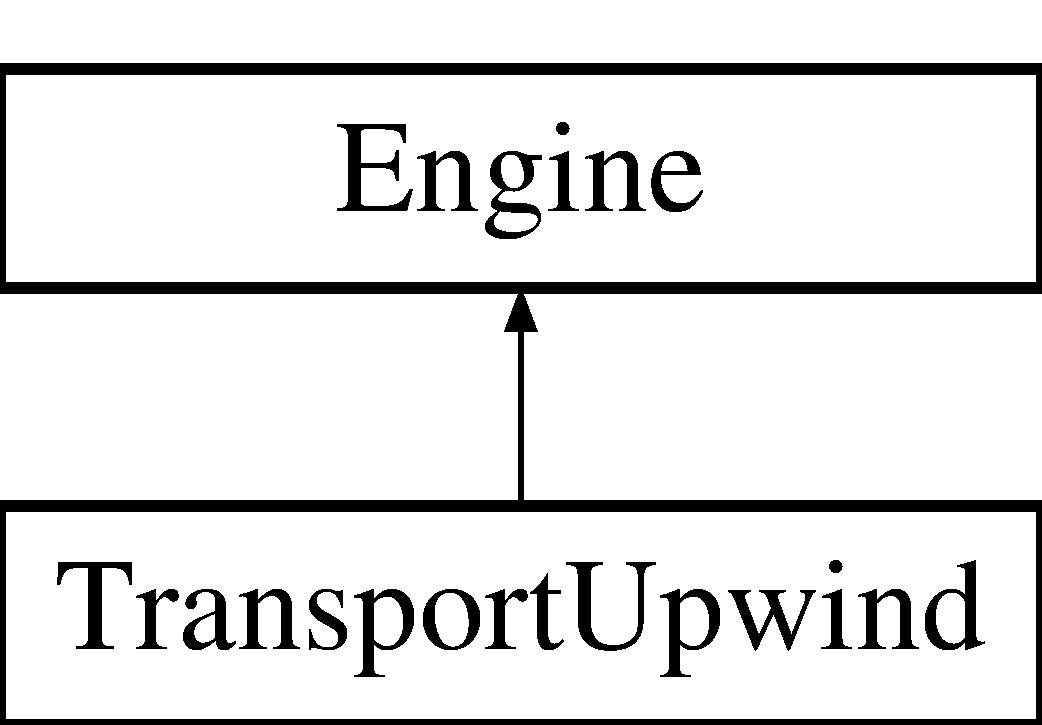
\includegraphics[height=2.000000cm]{classEngine}
\end{center}
\end{figure}
\subsection*{Public Member Functions}
\begin{DoxyCompactItemize}
\item 
\mbox{\Hypertarget{classEngine_a8c98683b0a3aa28d8ab72a8bcd0d52f2}\label{classEngine_a8c98683b0a3aa28d8ab72a8bcd0d52f2}} 
\mbox{\hyperlink{classEngine_a8c98683b0a3aa28d8ab72a8bcd0d52f2}{Engine}} ()
\begin{DoxyCompactList}\small\item\em Constructor. \end{DoxyCompactList}\item 
\mbox{\Hypertarget{classEngine_a8ef7030a089ecb30bbfcb9e43094717a}\label{classEngine_a8ef7030a089ecb30bbfcb9e43094717a}} 
\mbox{\hyperlink{classEngine_a8ef7030a089ecb30bbfcb9e43094717a}{$\sim$\+Engine}} ()
\begin{DoxyCompactList}\small\item\em Destructor. \end{DoxyCompactList}\item 
\mbox{\Hypertarget{classEngine_a8464ed1410156a3ccff819373c914297}\label{classEngine_a8464ed1410156a3ccff819373c914297}} 
int \mbox{\hyperlink{classEngine_a8464ed1410156a3ccff819373c914297}{main}} (int argc, char $\ast$$\ast$argv)
\begin{DoxyCompactList}\small\item\em Main function of program, calls init and start function of the inherited engine. \end{DoxyCompactList}\item 
\mbox{\Hypertarget{classEngine_add639334c809cd3e5c5888899df08e39}\label{classEngine_add639334c809cd3e5c5888899df08e39}} 
virtual int \mbox{\hyperlink{classEngine_add639334c809cd3e5c5888899df08e39}{init}} ()=0
\begin{DoxyCompactList}\small\item\em Virtual init function. Program here all necessary init procedures. \end{DoxyCompactList}\item 
\mbox{\Hypertarget{classEngine_a133fbaf71f1fb7a2c7eccc9f3482e923}\label{classEngine_a133fbaf71f1fb7a2c7eccc9f3482e923}} 
virtual int \mbox{\hyperlink{classEngine_a133fbaf71f1fb7a2c7eccc9f3482e923}{start}} ()=0
\begin{DoxyCompactList}\small\item\em Virtual start function. Program here the iterations of the scheme. \end{DoxyCompactList}\item 
\mbox{\Hypertarget{classEngine_a1b3dc669e0b686b4d2f32d57f980b7bd}\label{classEngine_a1b3dc669e0b686b4d2f32d57f980b7bd}} 
virtual int {\bfseries finalize} ()=0
\item 
void \mbox{\hyperlink{classEngine_a6837cf148e122390a924718435cea117}{set\+Options}} (real T, real C\+FL)
\begin{DoxyCompactList}\small\item\em Set scheme options \+: final time and Courant-\/\+Friedrichs-\/\+Levy condition. \end{DoxyCompactList}\item 
\mbox{\Hypertarget{classEngine_afca31326a5716439b2d0303cc9888cc5}\label{classEngine_afca31326a5716439b2d0303cc9888cc5}} 
void {\bfseries update\+Domain\+Uxmax} ()
\item 
\mbox{\Hypertarget{classEngine_ab6dee2316ca22ea528cd49fdb397f25c}\label{classEngine_ab6dee2316ca22ea528cd49fdb397f25c}} 
void {\bfseries update\+Domain\+Uymax} ()
\end{DoxyCompactItemize}
\subsection*{Protected Attributes}
\begin{DoxyCompactItemize}
\item 
\mbox{\Hypertarget{classEngine_ae12535c5ba837c7ea2636f76678132fe}\label{classEngine_ae12535c5ba837c7ea2636f76678132fe}} 
std\+::string {\bfseries \+\_\+initpath}
\item 
\mbox{\Hypertarget{classEngine_adf268ff3f02e5c4a4d9e987c5eb1d925}\label{classEngine_adf268ff3f02e5c4a4d9e987c5eb1d925}} 
std\+::string {\bfseries \+\_\+outputpath}
\item 
\mbox{\Hypertarget{classEngine_a63dbd1e0bcf5221273e991676ada9811}\label{classEngine_a63dbd1e0bcf5221273e991676ada9811}} 
int {\bfseries \+\_\+test\+Flag}
\item 
\mbox{\Hypertarget{classEngine_a30cd2cb8cf89a468f09b28109e91104d}\label{classEngine_a30cd2cb8cf89a468f09b28109e91104d}} 
int {\bfseries \+\_\+dry\+Flag}
\item 
\mbox{\Hypertarget{classEngine_ad868f62c35249da60df7aba62151e6dd}\label{classEngine_ad868f62c35249da60df7aba62151e6dd}} 
real {\bfseries \+\_\+T}
\item 
\mbox{\Hypertarget{classEngine_a1c37d4f8d2f9c46afeb5356bb496bde4}\label{classEngine_a1c37d4f8d2f9c46afeb5356bb496bde4}} 
real {\bfseries \+\_\+\+C\+FL}
\item 
\mbox{\Hypertarget{classEngine_a08555133228ffdf91eca97451f777ef2}\label{classEngine_a08555133228ffdf91eca97451f777ef2}} 
\mbox{\hyperlink{classTimer}{Timer}} {\bfseries \+\_\+timer}
\item 
\mbox{\Hypertarget{classEngine_a4e9850fba1cc1df1ab81d5ea6b9f6c82}\label{classEngine_a4e9850fba1cc1df1ab81d5ea6b9f6c82}} 
int {\bfseries \+\_\+\+M\+P\+I\+\_\+rank}
\item 
\mbox{\Hypertarget{classEngine_aa06c4f3111e2fe70888af5b6b9fdbdde}\label{classEngine_aa06c4f3111e2fe70888af5b6b9fdbdde}} 
std\+::vector$<$ real $>$ {\bfseries \+\_\+\+S\+D\+S\+\_\+uxmax}
\item 
\mbox{\Hypertarget{classEngine_a25d40c496dff6801e1b8b52eadd4a893}\label{classEngine_a25d40c496dff6801e1b8b52eadd4a893}} 
std\+::vector$<$ real $>$ {\bfseries \+\_\+\+S\+D\+S\+\_\+uymax}
\item 
\mbox{\Hypertarget{classEngine_ab6c4104db16ab3201e34af695c3492c1}\label{classEngine_ab6c4104db16ab3201e34af695c3492c1}} 
real {\bfseries \+\_\+\+S\+D\+D\+\_\+uxmax}
\item 
\mbox{\Hypertarget{classEngine_a9e1542346fb28c0a2cb9ea02640f1f94}\label{classEngine_a9e1542346fb28c0a2cb9ea02640f1f94}} 
real {\bfseries \+\_\+\+S\+D\+D\+\_\+uymax}
\item 
\mbox{\Hypertarget{classEngine_a4286013e363e097cae5a7f4df4b86b56}\label{classEngine_a4286013e363e097cae5a7f4df4b86b56}} 
real {\bfseries \+\_\+\+Domain\+\_\+uxmax}
\item 
\mbox{\Hypertarget{classEngine_ad9b42c6947ad96fecb3e1e6102471f17}\label{classEngine_ad9b42c6947ad96fecb3e1e6102471f17}} 
real {\bfseries \+\_\+\+Domain\+\_\+uymax}
\item 
\mbox{\Hypertarget{classEngine_a419970715d830fa99907c4f195863297}\label{classEngine_a419970715d830fa99907c4f195863297}} 
unsigned int {\bfseries \+\_\+n\+Iterations}
\end{DoxyCompactItemize}


\subsection{Detailed Description}
base class used to program a numerical scheme 

\subsection{Member Function Documentation}
\mbox{\Hypertarget{classEngine_a6837cf148e122390a924718435cea117}\label{classEngine_a6837cf148e122390a924718435cea117}} 
\index{Engine@{Engine}!set\+Options@{set\+Options}}
\index{set\+Options@{set\+Options}!Engine@{Engine}}
\subsubsection{\texorpdfstring{set\+Options()}{setOptions()}}
{\footnotesize\ttfamily void Engine\+::set\+Options (\begin{DoxyParamCaption}\item[{real}]{T,  }\item[{real}]{C\+FL }\end{DoxyParamCaption})}



Set scheme options \+: final time and Courant-\/\+Friedrichs-\/\+Levy condition. 


\begin{DoxyParams}{Parameters}
{\em T} & final time \\
\hline
{\em C\+FL} & Courant-\/\+Friedrichs-\/\+Levy condition \\
\hline
\end{DoxyParams}


The documentation for this class was generated from the following files\+:\begin{DoxyCompactItemize}
\item 
source/engine/\mbox{\hyperlink{engine_8hpp}{engine.\+hpp}}\item 
source/engine/engine.\+cpp\end{DoxyCompactItemize}

\hypertarget{classException}{}\section{Exception Class Reference}
\label{classException}\index{Exception@{Exception}}
Inheritance diagram for Exception\+:\begin{figure}[H]
\begin{center}
\leavevmode
\includegraphics[height=2.000000cm]{classException}
\end{center}
\end{figure}
\subsection*{Public Member Functions}
\begin{DoxyCompactItemize}
\item 
\mbox{\Hypertarget{classException_afed32696646800f73466d765b785cf3c}\label{classException_afed32696646800f73466d765b785cf3c}} 
{\footnotesize template$<$typename T $>$ }\\{\bfseries Exception} (const char $\ast$fil, int lin, T const \&msg)
\item 
\mbox{\Hypertarget{classException_a8be0f3d62682991241ae7a097d73f8fe}\label{classException_a8be0f3d62682991241ae7a097d73f8fe}} 
{\footnotesize template$<$typename T , typename... Args$>$ }\\{\bfseries Exception} (const char $\ast$fil, int lin, const char $\ast$msg, const T \&value, Args... args)
\item 
\mbox{\Hypertarget{classException_add710fe2bae3ac497ed60393eea35c91}\label{classException_add710fe2bae3ac497ed60393eea35c91}} 
const char $\ast$ {\bfseries what} () const  throw ()
\end{DoxyCompactItemize}


The documentation for this class was generated from the following file\+:\begin{DoxyCompactItemize}
\item 
source/toolkit/exception/exception.\+hpp\end{DoxyCompactItemize}

\hypertarget{classGeometry}{
\section{Geometry Class Reference}
\label{classGeometry}\index{Geometry@{Geometry}}
}


Tool providing various splits of SDDs (rectangular shapes) into SDS (any shape).  


{\ttfamily \#include $<$Geometry.hpp$>$}\subsection*{Public Member Functions}
\begin{DoxyCompactItemize}
\item 
\hyperlink{classGeometry_ac7e6a2114a9969257aa18147575cd2fb}{Geometry} (int bottomLeftX, int bottomLeftY, unsigned int sizeX, unsigned int sizeY)
\item 
std::vector$<$ std::vector$<$ std::pair$<$ int, int $>$ $>$ $>$ \hyperlink{classGeometry_a64fa42fab5fe0c5e9bb7d960bafa55fd}{buildGeometry} (unsigned int nShapes, std::string geomType)
\end{DoxyCompactItemize}
\subsection*{Static Public Attributes}
\begin{DoxyCompactItemize}
\item 
\hypertarget{classGeometry_a58cd0d80518f153a1e219140cb91980b}{
static const std::string {\bfseries LINE} = \char`\"{}line\char`\"{}}
\label{classGeometry_a58cd0d80518f153a1e219140cb91980b}

\item 
\hypertarget{classGeometry_a914bf3bdc008a1651aa315c4dd47318d}{
static const std::string {\bfseries RECTANGLE} = \char`\"{}rectangle\char`\"{}}
\label{classGeometry_a914bf3bdc008a1651aa315c4dd47318d}

\item 
\hypertarget{classGeometry_a6ac0d43e3e3e040bb7b2d1aacd2c7491}{
static const std::string {\bfseries RANDOM} = \char`\"{}random\char`\"{}}
\label{classGeometry_a6ac0d43e3e3e040bb7b2d1aacd2c7491}

\item 
\hypertarget{classGeometry_a4a7f3e4300ea2d63741981a6265b75bd}{
static const std::string {\bfseries DIAGONAL} = \char`\"{}diagonal\char`\"{}}
\label{classGeometry_a4a7f3e4300ea2d63741981a6265b75bd}

\item 
\hypertarget{classGeometry_ac7c81afa8454187adc7be4e7b7f68d3c}{
static const std::string {\bfseries TRIANGLE} = \char`\"{}triangle\char`\"{}}
\label{classGeometry_ac7c81afa8454187adc7be4e7b7f68d3c}

\item 
\hypertarget{classGeometry_ad93926a0e530cc7e85a79ebc9da99b32}{
static const std::string {\bfseries AMR} = \char`\"{}amr\char`\"{}}
\label{classGeometry_ad93926a0e530cc7e85a79ebc9da99b32}

\end{DoxyCompactItemize}


\subsection{Detailed Description}
Tool providing various splits of SDDs (rectangular shapes) into SDS (any shape). 

\subsection{Constructor \& Destructor Documentation}
\hypertarget{classGeometry_ac7e6a2114a9969257aa18147575cd2fb}{
\index{Geometry@{Geometry}!Geometry@{Geometry}}
\index{Geometry@{Geometry}!Geometry@{Geometry}}
\subsubsection[{Geometry}]{\setlength{\rightskip}{0pt plus 5cm}Geometry::Geometry (int {\em bottomLeftX}, \/  int {\em bottomLeftY}, \/  unsigned int {\em sizeX}, \/  unsigned int {\em sizeY})}}
\label{classGeometry_ac7e6a2114a9969257aa18147575cd2fb}
Constructor


\begin{DoxyParams}{Parameters}
\item[{\em bottomLeftX}]X-\/coord of bottem-\/left point of SDD \item[{\em bottomLeftX}]Y-\/coord of bottem-\/left point of SDD \item[{\em sizeX}]width of SDD \item[{\em sizeY}]height of SDD \end{DoxyParams}


\subsection{Member Function Documentation}
\hypertarget{classGeometry_a64fa42fab5fe0c5e9bb7d960bafa55fd}{
\index{Geometry@{Geometry}!buildGeometry@{buildGeometry}}
\index{buildGeometry@{buildGeometry}!Geometry@{Geometry}}
\subsubsection[{buildGeometry}]{\setlength{\rightskip}{0pt plus 5cm}std::vector$<$ std::vector$<$ std::pair$<$ int, int $>$ $>$ $>$ Geometry::buildGeometry (unsigned int {\em nShapes}, \/  std::string {\em geomType})}}
\label{classGeometry_a64fa42fab5fe0c5e9bb7d960bafa55fd}
build \hyperlink{classGeometry}{Geometry} according to number and type of shapes


\begin{DoxyParams}{Parameters}
\item[{\em nShapes}]number of SDS shapes to create \item[{\em geomType}]type of geometry to build \end{DoxyParams}


The documentation for this class was generated from the following files:\begin{DoxyCompactItemize}
\item 
subdomain/\hyperlink{Geometry_8hpp}{Geometry.hpp}\item 
subdomain/Geometry.cpp\end{DoxyCompactItemize}

\hypertarget{classQuantity}{}\section{Quantity$<$ T $>$ Class Template Reference}
\label{classQuantity}\index{Quantity$<$ T $>$@{Quantity$<$ T $>$}}


Physical quantity used in numerical schemes.  




{\ttfamily \#include $<$Quantity.\+hpp$>$}

\subsection*{Public Member Functions}
\begin{DoxyCompactItemize}
\item 
\mbox{\hyperlink{classQuantity_ab07b278cfe453e82756684b1730efc95}{Quantity}} (unsigned int size, const \mbox{\hyperlink{classCoordConverter}{Coord\+Converter}} \&coord\+Converter)
\begin{DoxyCompactList}\small\item\em Constructor. \end{DoxyCompactList}\item 
const T \& \mbox{\hyperlink{classQuantity_ac89252c633f43297f2df6fd6291c94b4}{get}} (unsigned int n, int coordX, int coordY) const
\begin{DoxyCompactList}\small\item\em Returns desired data available for reading and writing using the S\+DD\textquotesingle{}s coord converter. \end{DoxyCompactList}\item 
void \mbox{\hyperlink{classQuantity_a10c68498d1dfe59535a6f07c0627c8d4}{set}} (T value, unsigned int n, int coordX, int coordY)
\begin{DoxyCompactList}\small\item\em Returns desired data available for reading and writing using a specific S\+DS\textquotesingle{}s coord converter (see class \mbox{\hyperlink{classSDShared}{S\+D\+Shared}}) \end{DoxyCompactList}\item 
\mbox{\Hypertarget{classQuantity_af0799b7702ab9c7724399a6d76a41ea9}\label{classQuantity_af0799b7702ab9c7724399a6d76a41ea9}} 
void \mbox{\hyperlink{classQuantity_af0799b7702ab9c7724399a6d76a41ea9}{switch\+Prev\+Next}} ()
\begin{DoxyCompactList}\small\item\em To be called when an iteration is done to switch between arrays of data. \end{DoxyCompactList}\item 
\mbox{\Hypertarget{classQuantity_a0695a0b97d36ea8c39538f6156f0a878}\label{classQuantity_a0695a0b97d36ea8c39538f6156f0a878}} 
int {\bfseries current\+Prev} () const
\item 
\mbox{\Hypertarget{classQuantity_ad02771a40d16a4c293af97a4fd523d57}\label{classQuantity_ad02771a40d16a4c293af97a4fd523d57}} 
const T \& {\bfseries get0} (size\+\_\+t pos) const
\item 
\mbox{\Hypertarget{classQuantity_aae08f6fa99d0b180586f0bc3b7a79682}\label{classQuantity_aae08f6fa99d0b180586f0bc3b7a79682}} 
const T \& {\bfseries get1} (size\+\_\+t pos) const
\item 
\mbox{\Hypertarget{classQuantity_a0c6e6842590a156a1d79dacc0b5400bf}\label{classQuantity_a0c6e6842590a156a1d79dacc0b5400bf}} 
void {\bfseries set0} (T value, size\+\_\+t pos)
\item 
\mbox{\Hypertarget{classQuantity_aefb1880eb7f32e0ec0fb05430032168b}\label{classQuantity_aefb1880eb7f32e0ec0fb05430032168b}} 
void {\bfseries set1} (T value, size\+\_\+t pos)
\end{DoxyCompactItemize}


\subsection{Detailed Description}
\subsubsection*{template$<$typename T$>$\newline
class Quantity$<$ T $>$}

Physical quantity used in numerical schemes. 

Templated class defining a physical quantity of a certain size to be defined on the discrete domain, and its storage in memory. The typename defines the type of the stored values. It contains two arrays of data as required by a scheme of order 1 in time, and switches between them to avoid unnecesary writing. 

\subsection{Constructor \& Destructor Documentation}
\mbox{\Hypertarget{classQuantity_ab07b278cfe453e82756684b1730efc95}\label{classQuantity_ab07b278cfe453e82756684b1730efc95}} 
\index{Quantity@{Quantity}!Quantity@{Quantity}}
\index{Quantity@{Quantity}!Quantity@{Quantity}}
\subsubsection{\texorpdfstring{Quantity()}{Quantity()}}
{\footnotesize\ttfamily template$<$typename T $>$ \\
\mbox{\hyperlink{classQuantity}{Quantity}}$<$ T $>$\+::\mbox{\hyperlink{classQuantity}{Quantity}} (\begin{DoxyParamCaption}\item[{unsigned int}]{size,  }\item[{const \mbox{\hyperlink{classCoordConverter}{Coord\+Converter}} \&}]{coord\+Converter }\end{DoxyParamCaption})}



Constructor. 


\begin{DoxyParams}{Parameters}
{\em size} & \+: size of the created array \\
\hline
{\em coord\+Converter} & \+: tool linking coordinates of a cell/node to the corresponding memory index \\
\hline
\end{DoxyParams}


\subsection{Member Function Documentation}
\mbox{\Hypertarget{classQuantity_ac89252c633f43297f2df6fd6291c94b4}\label{classQuantity_ac89252c633f43297f2df6fd6291c94b4}} 
\index{Quantity@{Quantity}!get@{get}}
\index{get@{get}!Quantity@{Quantity}}
\subsubsection{\texorpdfstring{get()}{get()}}
{\footnotesize\ttfamily template$<$typename T $>$ \\
const T \& \mbox{\hyperlink{classQuantity}{Quantity}}$<$ T $>$\+::get (\begin{DoxyParamCaption}\item[{unsigned int}]{n,  }\item[{int}]{coordX,  }\item[{int}]{coordY }\end{DoxyParamCaption}) const}



Returns desired data available for reading and writing using the S\+DD\textquotesingle{}s coord converter. 


\begin{DoxyParams}{Parameters}
{\em n} & \+: returns current data if n == 0, next data if n == 1 \\
\hline
{\em coordX} & \+: X-\/axis coordinate on domain \\
\hline
{\em coordY} & \+: Y-\/axis coordinate on domain\\
\hline
\end{DoxyParams}
\begin{DoxyReturn}{Returns}
reference to the desired data 
\end{DoxyReturn}
\mbox{\Hypertarget{classQuantity_a10c68498d1dfe59535a6f07c0627c8d4}\label{classQuantity_a10c68498d1dfe59535a6f07c0627c8d4}} 
\index{Quantity@{Quantity}!set@{set}}
\index{set@{set}!Quantity@{Quantity}}
\subsubsection{\texorpdfstring{set()}{set()}}
{\footnotesize\ttfamily template$<$typename T$>$ \\
void \mbox{\hyperlink{classQuantity}{Quantity}}$<$ T $>$\+::set (\begin{DoxyParamCaption}\item[{T}]{value,  }\item[{unsigned int}]{n,  }\item[{int}]{coordX,  }\item[{int}]{coordY }\end{DoxyParamCaption})}



Returns desired data available for reading and writing using a specific S\+DS\textquotesingle{}s coord converter (see class \mbox{\hyperlink{classSDShared}{S\+D\+Shared}}) 


\begin{DoxyParams}{Parameters}
{\em n} & \+: returns previous data if n == 0, next data if n == 1 \\
\hline
{\em coordX} & \+: X-\/axis coordinate on domain \\
\hline
{\em coordY} & \+: Y-\/axis coordinate on domain\\
\hline
\end{DoxyParams}
\begin{DoxyReturn}{Returns}
reference to the desired data 
\end{DoxyReturn}


The documentation for this class was generated from the following file\+:\begin{DoxyCompactItemize}
\item 
source/subdomain/\mbox{\hyperlink{Quantity_8hpp}{Quantity.\+hpp}}\end{DoxyCompactItemize}

\hypertarget{classQuantityInterface}{
\section{QuantityInterface Class Reference}
\label{classQuantityInterface}\index{QuantityInterface@{QuantityInterface}}
}


Interface for storing multi-\/type quantity in the same array.  


{\ttfamily \#include $<$Quantity.hpp$>$}Inheritance diagram for QuantityInterface::\begin{figure}[H]
\begin{center}
\leavevmode
\includegraphics[height=2cm]{classQuantityInterface}
\end{center}
\end{figure}
\subsection*{Public Member Functions}
\begin{DoxyCompactItemize}
\item 
virtual \hyperlink{classQuantityInterface_acb39ddd398f6d615f28051bb32c25bbe}{$\sim$QuantityInterface} ()
\end{DoxyCompactItemize}


\subsection{Detailed Description}
Interface for storing multi-\/type quantity in the same array. 

\subsection{Constructor \& Destructor Documentation}
\hypertarget{classQuantityInterface_acb39ddd398f6d615f28051bb32c25bbe}{
\index{QuantityInterface@{QuantityInterface}!$\sim$QuantityInterface@{$\sim$QuantityInterface}}
\index{$\sim$QuantityInterface@{$\sim$QuantityInterface}!QuantityInterface@{QuantityInterface}}
\subsubsection[{$\sim$QuantityInterface}]{\setlength{\rightskip}{0pt plus 5cm}virtual QuantityInterface::$\sim$QuantityInterface ()\hspace{0.3cm}{\ttfamily  \mbox{[}inline, virtual\mbox{]}}}}
\label{classQuantityInterface_acb39ddd398f6d615f28051bb32c25bbe}
Virtual destructor 

The documentation for this class was generated from the following file:\begin{DoxyCompactItemize}
\item 
subdomain/\hyperlink{Quantity_8hpp}{Quantity.hpp}\end{DoxyCompactItemize}

\hypertarget{classSDDistributed}{}\section{S\+D\+Distributed Class Reference}
\label{classSDDistributed}\index{S\+D\+Distributed@{S\+D\+Distributed}}


Subdomain on distributed memory (S\+DD)  




{\ttfamily \#include $<$S\+D\+Distributed.\+hpp$>$}

\subsection*{Public Member Functions}
\begin{DoxyCompactItemize}
\item 
\hyperlink{classSDDistributed_a4ba8b15a2b28fcbf04d3665075918510}{S\+D\+Distributed} (unsigned int sizeX, unsigned int sizeY, int B\+L\+\_\+X, int B\+L\+\_\+Y, unsigned int boundary\+Thickness, unsigned int id, unsigned int n\+S\+DD)
\begin{DoxyCompactList}\small\item\em Constructor. \end{DoxyCompactList}\item 
\mbox{\Hypertarget{classSDDistributed_a1af9779279416a7bd519747e3b029124}\label{classSDDistributed_a1af9779279416a7bd519747e3b029124}} 
\hyperlink{classSDDistributed_a1af9779279416a7bd519747e3b029124}{$\sim$\+S\+D\+Distributed} ()
\begin{DoxyCompactList}\small\item\em Destructor. \end{DoxyCompactList}\item 
\mbox{\Hypertarget{classSDDistributed_a3617b83f6f2a6368b1f17c938d921e0a}\label{classSDDistributed_a3617b83f6f2a6368b1f17c938d921e0a}} 
std\+::map$<$ std\+::pair$<$ int, int $>$, std\+::pair$<$ int, std\+::pair$<$ int, int $>$ $>$ $>$ \hyperlink{classSDDistributed_a3617b83f6f2a6368b1f17c938d921e0a}{get\+Boundary\+Map} ()
\begin{DoxyCompactList}\small\item\em Returns map between coords on S\+DD and \char`\"{}real cell\char`\"{} on neighbour S\+DD / boundary side. \end{DoxyCompactList}\item 
\hyperlink{classQuantity}{Quantity}$<$ real $>$ $\ast$ \hyperlink{classSDDistributed_a14f296606ff1afa1e4878fa6c4928afc}{get\+Quantity} (std\+::string name)
\begin{DoxyCompactList}\small\item\em Gets physical quantity previously added with method add\+Quantity. \end{DoxyCompactList}\item 
const std\+::vector$<$ \hyperlink{classSDShared}{S\+D\+Shared} $>$ \& \hyperlink{classSDDistributed_a9afba0607b6012a0e446b95251559f5d}{get\+S\+DS} () const
\begin{DoxyCompactList}\small\item\em Gets all S\+DS on S\+DD for a read-\/only access. \end{DoxyCompactList}\item 
unsigned int \hyperlink{classSDDistributed_a567b9535558271515166ce7ebd3f6c29}{get\+SizeX} () const
\begin{DoxyCompactList}\small\item\em Gets width of S\+DD, excluding boundary thickness. \end{DoxyCompactList}\item 
unsigned int \hyperlink{classSDDistributed_a9bf0049f4c95513b4d9c9a9bac0f6eb4}{get\+SizeY} () const
\begin{DoxyCompactList}\small\item\em Gets height of S\+DD, excluding boundary thickness. \end{DoxyCompactList}\item 
unsigned int \hyperlink{classSDDistributed_a0ab71d942dca319b739390055942a96a}{get\+Id} () const
\begin{DoxyCompactList}\small\item\em Gets unique id of S\+DD. \end{DoxyCompactList}\item 
\mbox{\Hypertarget{classSDDistributed_a8a7bf55ebead74e2c234fe21ebc02475}\label{classSDDistributed_a8a7bf55ebead74e2c234fe21ebc02475}} 
unsigned int {\bfseries get\+Number\+Neighbour\+S\+D\+Ds} () const
\item 
\mbox{\Hypertarget{classSDDistributed_a9fe968b07308e670e2bc53597d2d139f}\label{classSDDistributed_a9fe968b07308e670e2bc53597d2d139f}} 
unsigned int {\bfseries get\+Number\+Overlap\+Cells} () const
\item 
\mbox{\Hypertarget{classSDDistributed_ad8247f4958820ef02d97e22059ee7f94}\label{classSDDistributed_ad8247f4958820ef02d97e22059ee7f94}} 
unsigned int {\bfseries get\+Number\+Boundary\+Cells} () const
\item 
const std\+::map$<$ std\+::pair$<$ int, int $>$, std\+::pair$<$ int, std\+::pair$<$ int, int $>$ $>$ $>$ \& \hyperlink{classSDDistributed_a5ca6adae6bc3b93f937a633f8813fed0}{get\+Overlap\+Cell\+Map} () const
\begin{DoxyCompactList}\small\item\em Returns mapping between overlap cells and corresponding \char`\"{}real cells\char`\"{} on other S\+D\+Ds. \end{DoxyCompactList}\item 
void \hyperlink{classSDDistributed_ae9d8db949ba9da0a95407e1066df17b9}{set\+Value} (std\+::string quantity\+Name, int coordX, int coordY, real value)
\begin{DoxyCompactList}\small\item\em Manually set the value on a coordinate, without having to get the quantity. \end{DoxyCompactList}\item 
real \hyperlink{classSDDistributed_a1db6a1bf2f8781b9e4b12be99b4bf9c4}{get\+Value} (std\+::string quantity\+Name, int coordX, int coordY) const
\begin{DoxyCompactList}\small\item\em Manually set the value on a coordinate, without having to get the quantity. \end{DoxyCompactList}\item 
void \hyperlink{classSDDistributed_ae7695b6c9096e7a2f9c5fc16174aaae9}{build\+Send\+Map} (const \hyperlink{classDomain}{Domain} \&domain)
\begin{DoxyCompactList}\small\item\em Builds map of cells to send from this S\+DD to other S\+D\+Ds. \end{DoxyCompactList}\item 
void \hyperlink{classSDDistributed_af819b64d742bec7dee4fd0fab43aa6e5}{build\+Recv\+Map} (const \hyperlink{classDomain}{Domain} \&domain)
\begin{DoxyCompactList}\small\item\em Builds map between coords on S\+DD and \char`\"{}real cell\char`\"{} on neighbour S\+DD / boundary side. \end{DoxyCompactList}\item 
{\footnotesize template$<$typename T $>$ }\\void \hyperlink{classSDDistributed_a82b5a390e964051d1952c683b4fa5f05}{add\+Quantity} (std\+::string name)
\begin{DoxyCompactList}\small\item\em Adds physical quantity (and thus data) used in the scheme. \end{DoxyCompactList}\item 
void \hyperlink{classSDDistributed_a3dbacea02c2d4f36310c81f87f90fe5a}{build\+All\+S\+DS} (unsigned int n\+S\+DS, std\+::string geom\+Type)
\begin{DoxyCompactList}\small\item\em Build subdomains on shared memory based on geometry type. \end{DoxyCompactList}\item 
void \hyperlink{classSDDistributed_a467f8c05c2cf7728828ec9d0c617e667}{update\+Overlap\+Cells} (const std\+::vector$<$ std\+::string $>$ \&qties\+To\+Update)
\begin{DoxyCompactList}\small\item\em Updates overlap cells by communicating through M\+PI with other S\+D\+Ds. \end{DoxyCompactList}\item 
void \hyperlink{classSDDistributed_a492c6799b5b1f79481a2ee6e50979a18}{update\+Neumann\+Cells} (std\+::string quantity\+Name, bool change\+To\+Opposite=false)
\begin{DoxyCompactList}\small\item\em Updates Neumann boundary cells of S\+DD according to values stored in memory. \end{DoxyCompactList}\item 
void \hyperlink{classSDDistributed_a0eaa89db3fd4b663d887de8dcf9f65af}{update\+Dirichlet\+Cells} (std\+::string quantity\+Name)
\begin{DoxyCompactList}\small\item\em Updates Dirichlet boundary cells of S\+DD according to values stored in memory. \end{DoxyCompactList}\item 
void \hyperlink{classSDDistributed_a0974e2cce9bfcddfd0acccd1105d980f}{add\+Equation} (std\+::string eq\+Name, eq\+Type eq\+Func)
\begin{DoxyCompactList}\small\item\em Adds an equation to the stack of equations to be computed by the scheme. \end{DoxyCompactList}\item 
\mbox{\Hypertarget{classSDDistributed_a00a539076c306457a4dd1aef2c4f2039}\label{classSDDistributed_a00a539076c306457a4dd1aef2c4f2039}} 
void \hyperlink{classSDDistributed_a00a539076c306457a4dd1aef2c4f2039}{exec\+Equation} (std\+::string eq\+Name)
\begin{DoxyCompactList}\small\item\em Computes equation in the order they were added to the task stack. \end{DoxyCompactList}\item 
void \hyperlink{classSDDistributed_a75660cf18d7248ac64e86ab457061b91}{init\+Thread\+Pool} (unsigned int n\+Threads)
\begin{DoxyCompactList}\small\item\em Builds thread pool given an amount of threads to build. \end{DoxyCompactList}\item 
\hyperlink{classSDDistributed_a49ef3cd6d1409cc71d3800fd0fca2f28}{S\+D\+Distributed} (unsigned int sizeX, unsigned int sizeY, unsigned int boundary\+Thickness, unsigned int id)
\begin{DoxyCompactList}\small\item\em Constructor. \end{DoxyCompactList}\item 
\mbox{\Hypertarget{classSDDistributed_a1af9779279416a7bd519747e3b029124}\label{classSDDistributed_a1af9779279416a7bd519747e3b029124}} 
\hyperlink{classSDDistributed_a1af9779279416a7bd519747e3b029124}{$\sim$\+S\+D\+Distributed} ()
\begin{DoxyCompactList}\small\item\em Destructor. \end{DoxyCompactList}\item 
\mbox{\Hypertarget{classSDDistributed_a995e6fad585afbf4158ea0b323eafc76}\label{classSDDistributed_a995e6fad585afbf4158ea0b323eafc76}} 
void \hyperlink{classSDDistributed_a995e6fad585afbf4158ea0b323eafc76}{build\+Boundary\+Map} (const \hyperlink{classDomain}{Domain} \&domain)
\begin{DoxyCompactList}\small\item\em Builds map between coords on S\+DD and \char`\"{}real cell\char`\"{} on neighbour S\+DD / boundary side. \end{DoxyCompactList}\item 
\mbox{\Hypertarget{classSDDistributed_a3617b83f6f2a6368b1f17c938d921e0a}\label{classSDDistributed_a3617b83f6f2a6368b1f17c938d921e0a}} 
std\+::map$<$ std\+::pair$<$ int, int $>$, std\+::pair$<$ int, std\+::pair$<$ int, int $>$ $>$ $>$ \hyperlink{classSDDistributed_a3617b83f6f2a6368b1f17c938d921e0a}{get\+Boundary\+Map} ()
\begin{DoxyCompactList}\small\item\em Returns map between coords on S\+DD and \char`\"{}real cell\char`\"{} on neighbour S\+DD / boundary side. \end{DoxyCompactList}\item 
{\footnotesize template$<$typename T $>$ }\\void \hyperlink{classSDDistributed_a82b5a390e964051d1952c683b4fa5f05}{add\+Quantity} (std\+::string name)
\begin{DoxyCompactList}\small\item\em Adds physical quantity (and thus data) used in the scheme. \end{DoxyCompactList}\item 
\hyperlink{classQuantity}{Quantity}$<$ real $>$ $\ast$ \hyperlink{classSDDistributed_ade2c34b9bd189f3fb7409fc8dddd55ee}{get\+Quantity} (std\+::string name)
\begin{DoxyCompactList}\small\item\em Gets physical quantity previously added with method add\+Quantity. \end{DoxyCompactList}\item 
void \hyperlink{classSDDistributed_a3dbacea02c2d4f36310c81f87f90fe5a}{build\+All\+S\+DS} (unsigned int n\+S\+DS, std\+::string geom\+Type)
\begin{DoxyCompactList}\small\item\em Build subdomains on shared memory based on geometry type. \end{DoxyCompactList}\item 
const std\+::vector$<$ \hyperlink{classSDShared}{S\+D\+Shared} $>$ \& \hyperlink{classSDDistributed_a2bbdfc4e93476c4ee8cc0b55682a7a5b}{get\+S\+DS} () const
\begin{DoxyCompactList}\small\item\em Gets all S\+DS on S\+DD for a read-\/only access. \end{DoxyCompactList}\item 
unsigned int \hyperlink{classSDDistributed_a567b9535558271515166ce7ebd3f6c29}{get\+SizeX} () const
\begin{DoxyCompactList}\small\item\em Gets width of S\+DD. \end{DoxyCompactList}\item 
unsigned int \hyperlink{classSDDistributed_a9bf0049f4c95513b4d9c9a9bac0f6eb4}{get\+SizeY} () const
\begin{DoxyCompactList}\small\item\em Gets height of S\+DD. \end{DoxyCompactList}\item 
unsigned int \hyperlink{classSDDistributed_a0ab71d942dca319b739390055942a96a}{get\+Id} () const
\begin{DoxyCompactList}\small\item\em Gets unique id of S\+DD. \end{DoxyCompactList}\item 
const std\+::map$<$ std\+::pair$<$ int, int $>$, std\+::pair$<$ int, std\+::pair$<$ int, int $>$ $>$ $>$ \& \hyperlink{classSDDistributed_a2a2e744edad326561e3555a352ce4a0a}{get\+Overlap\+Cell\+Map} () const
\begin{DoxyCompactList}\small\item\em Returns mapping between overlap cells and corresponding \char`\"{}real cells\char`\"{} on other S\+D\+Ds. \end{DoxyCompactList}\item 
\mbox{\Hypertarget{classSDDistributed_a492c6799b5b1f79481a2ee6e50979a18}\label{classSDDistributed_a492c6799b5b1f79481a2ee6e50979a18}} 
void {\bfseries update\+Neumann\+Cells} (std\+::string quantity\+Name, bool change\+To\+Opposite=false)
\item 
\mbox{\Hypertarget{classSDDistributed_a0eaa89db3fd4b663d887de8dcf9f65af}\label{classSDDistributed_a0eaa89db3fd4b663d887de8dcf9f65af}} 
void {\bfseries update\+Dirichlet\+Cells} (std\+::string quantity\+Name)
\item 
\mbox{\Hypertarget{classSDDistributed_a4c8dc37fa1d0991f0b883563df329518}\label{classSDDistributed_a4c8dc37fa1d0991f0b883563df329518}} 
void {\bfseries add\+Equation} (eq\+Type eq\+Func)
\item 
\mbox{\Hypertarget{classSDDistributed_a083335cd910b0818fb0990873b4e1f87}\label{classSDDistributed_a083335cd910b0818fb0990873b4e1f87}} 
void {\bfseries exec\+Equation} ()
\item 
\mbox{\Hypertarget{classSDDistributed_a75660cf18d7248ac64e86ab457061b91}\label{classSDDistributed_a75660cf18d7248ac64e86ab457061b91}} 
void {\bfseries init\+Thread\+Pool} (unsigned int n\+Threads)
\end{DoxyCompactItemize}


\subsection{Detailed Description}
Subdomain on distributed memory (S\+DD) 

Defines a subdomain on distributed memory. It represents a part of a domain available as a single block of memory, hence its definition as a rectangle. It will then be sliced on geometric subdomains on this block of shared memory (\hyperlink{classSDShared}{S\+D\+Shared}). 

\subsection{Constructor \& Destructor Documentation}
\mbox{\Hypertarget{classSDDistributed_a4ba8b15a2b28fcbf04d3665075918510}\label{classSDDistributed_a4ba8b15a2b28fcbf04d3665075918510}} 
\index{S\+D\+Distributed@{S\+D\+Distributed}!S\+D\+Distributed@{S\+D\+Distributed}}
\index{S\+D\+Distributed@{S\+D\+Distributed}!S\+D\+Distributed@{S\+D\+Distributed}}
\subsubsection{\texorpdfstring{S\+D\+Distributed()}{SDDistributed()}\hspace{0.1cm}{\footnotesize\ttfamily [1/2]}}
{\footnotesize\ttfamily S\+D\+Distributed\+::\+S\+D\+Distributed (\begin{DoxyParamCaption}\item[{unsigned int}]{sizeX,  }\item[{unsigned int}]{sizeY,  }\item[{int}]{B\+L\+\_\+X,  }\item[{int}]{B\+L\+\_\+Y,  }\item[{unsigned int}]{boundary\+Thickness,  }\item[{unsigned int}]{id,  }\item[{unsigned int}]{n\+S\+DD }\end{DoxyParamCaption})}



Constructor. 


\begin{DoxyParams}{Parameters}
{\em sizeX} & number of cells of subdomain on the X-\/axis \\
\hline
{\em sizeY} & number of cells of subdomain on the Y-\/axis \\
\hline
\end{DoxyParams}
\mbox{\Hypertarget{classSDDistributed_a49ef3cd6d1409cc71d3800fd0fca2f28}\label{classSDDistributed_a49ef3cd6d1409cc71d3800fd0fca2f28}} 
\index{S\+D\+Distributed@{S\+D\+Distributed}!S\+D\+Distributed@{S\+D\+Distributed}}
\index{S\+D\+Distributed@{S\+D\+Distributed}!S\+D\+Distributed@{S\+D\+Distributed}}
\subsubsection{\texorpdfstring{S\+D\+Distributed()}{SDDistributed()}\hspace{0.1cm}{\footnotesize\ttfamily [2/2]}}
{\footnotesize\ttfamily S\+D\+Distributed\+::\+S\+D\+Distributed (\begin{DoxyParamCaption}\item[{unsigned int}]{sizeX,  }\item[{unsigned int}]{sizeY,  }\item[{unsigned int}]{boundary\+Thickness,  }\item[{unsigned int}]{id }\end{DoxyParamCaption})}



Constructor. 


\begin{DoxyParams}{Parameters}
{\em sizeX} & \+: number of cells of subdomain on the X-\/axis \\
\hline
{\em sizeY} & \+: number of cells of subdomain on the Y-\/axis \\
\hline
\end{DoxyParams}


\subsection{Member Function Documentation}
\mbox{\Hypertarget{classSDDistributed_a0974e2cce9bfcddfd0acccd1105d980f}\label{classSDDistributed_a0974e2cce9bfcddfd0acccd1105d980f}} 
\index{S\+D\+Distributed@{S\+D\+Distributed}!add\+Equation@{add\+Equation}}
\index{add\+Equation@{add\+Equation}!S\+D\+Distributed@{S\+D\+Distributed}}
\subsubsection{\texorpdfstring{add\+Equation()}{addEquation()}}
{\footnotesize\ttfamily void S\+D\+Distributed\+::add\+Equation (\begin{DoxyParamCaption}\item[{std\+::string}]{eq\+Name,  }\item[{eq\+Type}]{eq\+Func }\end{DoxyParamCaption})}



Adds an equation to the stack of equations to be computed by the scheme. 


\begin{DoxyParams}{Parameters}
{\em eq\+Func} & function to be added to the task \\
\hline
\end{DoxyParams}
\mbox{\Hypertarget{classSDDistributed_a82b5a390e964051d1952c683b4fa5f05}\label{classSDDistributed_a82b5a390e964051d1952c683b4fa5f05}} 
\index{S\+D\+Distributed@{S\+D\+Distributed}!add\+Quantity@{add\+Quantity}}
\index{add\+Quantity@{add\+Quantity}!S\+D\+Distributed@{S\+D\+Distributed}}
\subsubsection{\texorpdfstring{add\+Quantity()}{addQuantity()}\hspace{0.1cm}{\footnotesize\ttfamily [1/2]}}
{\footnotesize\ttfamily template$<$typename T $>$ \\
void S\+D\+Distributed\+::add\+Quantity (\begin{DoxyParamCaption}\item[{std\+::string}]{name }\end{DoxyParamCaption})}



Adds physical quantity (and thus data) used in the scheme. 


\begin{DoxyParams}{Parameters}
{\em name} & \+: name of the quantity to add \\
\hline
\end{DoxyParams}
\mbox{\Hypertarget{classSDDistributed_a82b5a390e964051d1952c683b4fa5f05}\label{classSDDistributed_a82b5a390e964051d1952c683b4fa5f05}} 
\index{S\+D\+Distributed@{S\+D\+Distributed}!add\+Quantity@{add\+Quantity}}
\index{add\+Quantity@{add\+Quantity}!S\+D\+Distributed@{S\+D\+Distributed}}
\subsubsection{\texorpdfstring{add\+Quantity()}{addQuantity()}\hspace{0.1cm}{\footnotesize\ttfamily [2/2]}}
{\footnotesize\ttfamily template$<$typename T $>$ \\
void S\+D\+Distributed\+::add\+Quantity (\begin{DoxyParamCaption}\item[{std\+::string}]{name }\end{DoxyParamCaption})}



Adds physical quantity (and thus data) used in the scheme. 


\begin{DoxyParams}{Parameters}
{\em name} & name of the quantity to add, used as reference when getting and setting a value, or when getting the whole quantity data \\
\hline
\end{DoxyParams}
\mbox{\Hypertarget{classSDDistributed_a3dbacea02c2d4f36310c81f87f90fe5a}\label{classSDDistributed_a3dbacea02c2d4f36310c81f87f90fe5a}} 
\index{S\+D\+Distributed@{S\+D\+Distributed}!build\+All\+S\+DS@{build\+All\+S\+DS}}
\index{build\+All\+S\+DS@{build\+All\+S\+DS}!S\+D\+Distributed@{S\+D\+Distributed}}
\subsubsection{\texorpdfstring{build\+All\+S\+D\+S()}{buildAllSDS()}\hspace{0.1cm}{\footnotesize\ttfamily [1/2]}}
{\footnotesize\ttfamily void S\+D\+Distributed\+::build\+All\+S\+DS (\begin{DoxyParamCaption}\item[{unsigned int}]{n\+S\+DS,  }\item[{std\+::string}]{geom\+Type }\end{DoxyParamCaption})}



Build subdomains on shared memory based on geometry type. 


\begin{DoxyParams}{Parameters}
{\em n\+S\+DS} & \+: number of subdomains to be built \\
\hline
{\em geom\+Type} & \+: geometry type of subdomain (see the \hyperlink{classGeometry}{Geometry} class for possible values) \\
\hline
\end{DoxyParams}
\mbox{\Hypertarget{classSDDistributed_a3dbacea02c2d4f36310c81f87f90fe5a}\label{classSDDistributed_a3dbacea02c2d4f36310c81f87f90fe5a}} 
\index{S\+D\+Distributed@{S\+D\+Distributed}!build\+All\+S\+DS@{build\+All\+S\+DS}}
\index{build\+All\+S\+DS@{build\+All\+S\+DS}!S\+D\+Distributed@{S\+D\+Distributed}}
\subsubsection{\texorpdfstring{build\+All\+S\+D\+S()}{buildAllSDS()}\hspace{0.1cm}{\footnotesize\ttfamily [2/2]}}
{\footnotesize\ttfamily void S\+D\+Distributed\+::build\+All\+S\+DS (\begin{DoxyParamCaption}\item[{unsigned int}]{n\+S\+DS,  }\item[{std\+::string}]{geom\+Type }\end{DoxyParamCaption})}



Build subdomains on shared memory based on geometry type. 


\begin{DoxyParams}{Parameters}
{\em n\+S\+DS} & number of subdomains to be built \\
\hline
{\em geom\+Type} & geometry type of subdomain (see the \hyperlink{classGeometry}{Geometry} class for possible values) \\
\hline
\end{DoxyParams}
\mbox{\Hypertarget{classSDDistributed_af819b64d742bec7dee4fd0fab43aa6e5}\label{classSDDistributed_af819b64d742bec7dee4fd0fab43aa6e5}} 
\index{S\+D\+Distributed@{S\+D\+Distributed}!build\+Recv\+Map@{build\+Recv\+Map}}
\index{build\+Recv\+Map@{build\+Recv\+Map}!S\+D\+Distributed@{S\+D\+Distributed}}
\subsubsection{\texorpdfstring{build\+Recv\+Map()}{buildRecvMap()}}
{\footnotesize\ttfamily void S\+D\+Distributed\+::build\+Recv\+Map (\begin{DoxyParamCaption}\item[{const \hyperlink{classDomain}{Domain} \&}]{domain }\end{DoxyParamCaption})}



Builds map between coords on S\+DD and \char`\"{}real cell\char`\"{} on neighbour S\+DD / boundary side. 


\begin{DoxyParams}{Parameters}
{\em domain} & parent domain of the S\+DD \\
\hline
\end{DoxyParams}
\mbox{\Hypertarget{classSDDistributed_ae7695b6c9096e7a2f9c5fc16174aaae9}\label{classSDDistributed_ae7695b6c9096e7a2f9c5fc16174aaae9}} 
\index{S\+D\+Distributed@{S\+D\+Distributed}!build\+Send\+Map@{build\+Send\+Map}}
\index{build\+Send\+Map@{build\+Send\+Map}!S\+D\+Distributed@{S\+D\+Distributed}}
\subsubsection{\texorpdfstring{build\+Send\+Map()}{buildSendMap()}}
{\footnotesize\ttfamily void S\+D\+Distributed\+::build\+Send\+Map (\begin{DoxyParamCaption}\item[{const \hyperlink{classDomain}{Domain} \&}]{domain }\end{DoxyParamCaption})}



Builds map of cells to send from this S\+DD to other S\+D\+Ds. 


\begin{DoxyParams}{Parameters}
{\em domain} & parent domain of the S\+DD \\
\hline
\end{DoxyParams}
\mbox{\Hypertarget{classSDDistributed_a0ab71d942dca319b739390055942a96a}\label{classSDDistributed_a0ab71d942dca319b739390055942a96a}} 
\index{S\+D\+Distributed@{S\+D\+Distributed}!get\+Id@{get\+Id}}
\index{get\+Id@{get\+Id}!S\+D\+Distributed@{S\+D\+Distributed}}
\subsubsection{\texorpdfstring{get\+Id()}{getId()}\hspace{0.1cm}{\footnotesize\ttfamily [1/2]}}
{\footnotesize\ttfamily unsigned int S\+D\+Distributed\+::get\+Id (\begin{DoxyParamCaption}{ }\end{DoxyParamCaption}) const}



Gets unique id of S\+DD. 

\begin{DoxyReturn}{Returns}
id of S\+DD 
\end{DoxyReturn}
\mbox{\Hypertarget{classSDDistributed_a0ab71d942dca319b739390055942a96a}\label{classSDDistributed_a0ab71d942dca319b739390055942a96a}} 
\index{S\+D\+Distributed@{S\+D\+Distributed}!get\+Id@{get\+Id}}
\index{get\+Id@{get\+Id}!S\+D\+Distributed@{S\+D\+Distributed}}
\subsubsection{\texorpdfstring{get\+Id()}{getId()}\hspace{0.1cm}{\footnotesize\ttfamily [2/2]}}
{\footnotesize\ttfamily unsigned int S\+D\+Distributed\+::get\+Id (\begin{DoxyParamCaption}{ }\end{DoxyParamCaption}) const}



Gets unique id of S\+DD. 

\begin{DoxyReturn}{Returns}
id of S\+DD 
\end{DoxyReturn}
\mbox{\Hypertarget{classSDDistributed_a2a2e744edad326561e3555a352ce4a0a}\label{classSDDistributed_a2a2e744edad326561e3555a352ce4a0a}} 
\index{S\+D\+Distributed@{S\+D\+Distributed}!get\+Overlap\+Cell\+Map@{get\+Overlap\+Cell\+Map}}
\index{get\+Overlap\+Cell\+Map@{get\+Overlap\+Cell\+Map}!S\+D\+Distributed@{S\+D\+Distributed}}
\subsubsection{\texorpdfstring{get\+Overlap\+Cell\+Map()}{getOverlapCellMap()}\hspace{0.1cm}{\footnotesize\ttfamily [1/2]}}
{\footnotesize\ttfamily const std\+::map$<$ std\+::pair$<$int, int$>$, std\+::pair$<$ int, std\+::pair$<$int, int$>$ $>$ $>$\& S\+D\+Distributed\+::get\+Overlap\+Cell\+Map (\begin{DoxyParamCaption}{ }\end{DoxyParamCaption}) const}



Returns mapping between overlap cells and corresponding \char`\"{}real cells\char`\"{} on other S\+D\+Ds. 

Used by the domain to communicate between S\+D\+Ds when updating overlap cells \mbox{\Hypertarget{classSDDistributed_a5ca6adae6bc3b93f937a633f8813fed0}\label{classSDDistributed_a5ca6adae6bc3b93f937a633f8813fed0}} 
\index{S\+D\+Distributed@{S\+D\+Distributed}!get\+Overlap\+Cell\+Map@{get\+Overlap\+Cell\+Map}}
\index{get\+Overlap\+Cell\+Map@{get\+Overlap\+Cell\+Map}!S\+D\+Distributed@{S\+D\+Distributed}}
\subsubsection{\texorpdfstring{get\+Overlap\+Cell\+Map()}{getOverlapCellMap()}\hspace{0.1cm}{\footnotesize\ttfamily [2/2]}}
{\footnotesize\ttfamily const std\+::map$<$ std\+::pair$<$ int, int $>$, std\+::pair$<$ int, std\+::pair$<$ int, int $>$ $>$ $>$ \& S\+D\+Distributed\+::get\+Overlap\+Cell\+Map (\begin{DoxyParamCaption}{ }\end{DoxyParamCaption}) const}



Returns mapping between overlap cells and corresponding \char`\"{}real cells\char`\"{} on other S\+D\+Ds. 

Used by the domain to communicate between S\+D\+Ds when updating overlap cells \mbox{\Hypertarget{classSDDistributed_ade2c34b9bd189f3fb7409fc8dddd55ee}\label{classSDDistributed_ade2c34b9bd189f3fb7409fc8dddd55ee}} 
\index{S\+D\+Distributed@{S\+D\+Distributed}!get\+Quantity@{get\+Quantity}}
\index{get\+Quantity@{get\+Quantity}!S\+D\+Distributed@{S\+D\+Distributed}}
\subsubsection{\texorpdfstring{get\+Quantity()}{getQuantity()}\hspace{0.1cm}{\footnotesize\ttfamily [1/2]}}
{\footnotesize\ttfamily \hyperlink{classQuantity}{Quantity}$<$real$>$$\ast$ S\+D\+Distributed\+::get\+Quantity (\begin{DoxyParamCaption}\item[{std\+::string}]{name }\end{DoxyParamCaption})}



Gets physical quantity previously added with method add\+Quantity. 


\begin{DoxyParams}{Parameters}
{\em name} & \+: name of the quantity to get \\
\hline
\end{DoxyParams}
\mbox{\Hypertarget{classSDDistributed_a14f296606ff1afa1e4878fa6c4928afc}\label{classSDDistributed_a14f296606ff1afa1e4878fa6c4928afc}} 
\index{S\+D\+Distributed@{S\+D\+Distributed}!get\+Quantity@{get\+Quantity}}
\index{get\+Quantity@{get\+Quantity}!S\+D\+Distributed@{S\+D\+Distributed}}
\subsubsection{\texorpdfstring{get\+Quantity()}{getQuantity()}\hspace{0.1cm}{\footnotesize\ttfamily [2/2]}}
{\footnotesize\ttfamily \hyperlink{classQuantity}{Quantity}$<$ real $>$ $\ast$ S\+D\+Distributed\+::get\+Quantity (\begin{DoxyParamCaption}\item[{std\+::string}]{name }\end{DoxyParamCaption})}



Gets physical quantity previously added with method add\+Quantity. 


\begin{DoxyParams}{Parameters}
{\em name} & name of the quantity to get \\
\hline
\end{DoxyParams}
\mbox{\Hypertarget{classSDDistributed_a2bbdfc4e93476c4ee8cc0b55682a7a5b}\label{classSDDistributed_a2bbdfc4e93476c4ee8cc0b55682a7a5b}} 
\index{S\+D\+Distributed@{S\+D\+Distributed}!get\+S\+DS@{get\+S\+DS}}
\index{get\+S\+DS@{get\+S\+DS}!S\+D\+Distributed@{S\+D\+Distributed}}
\subsubsection{\texorpdfstring{get\+S\+D\+S()}{getSDS()}\hspace{0.1cm}{\footnotesize\ttfamily [1/2]}}
{\footnotesize\ttfamily const std\+::vector$<$\hyperlink{classSDShared}{S\+D\+Shared}$>$\& S\+D\+Distributed\+::get\+S\+DS (\begin{DoxyParamCaption}{ }\end{DoxyParamCaption}) const}



Gets all S\+DS on S\+DD for a read-\/only access. 

\begin{DoxyReturn}{Returns}
const reference to the array of all subdomains on S\+DD 
\end{DoxyReturn}
\mbox{\Hypertarget{classSDDistributed_a9afba0607b6012a0e446b95251559f5d}\label{classSDDistributed_a9afba0607b6012a0e446b95251559f5d}} 
\index{S\+D\+Distributed@{S\+D\+Distributed}!get\+S\+DS@{get\+S\+DS}}
\index{get\+S\+DS@{get\+S\+DS}!S\+D\+Distributed@{S\+D\+Distributed}}
\subsubsection{\texorpdfstring{get\+S\+D\+S()}{getSDS()}\hspace{0.1cm}{\footnotesize\ttfamily [2/2]}}
{\footnotesize\ttfamily const std\+::vector$<$ \hyperlink{classSDShared}{S\+D\+Shared} $>$ \& S\+D\+Distributed\+::get\+S\+DS (\begin{DoxyParamCaption}{ }\end{DoxyParamCaption}) const}



Gets all S\+DS on S\+DD for a read-\/only access. 

\begin{DoxyReturn}{Returns}
const reference to the array of all subdomains on S\+DD 
\end{DoxyReturn}
\mbox{\Hypertarget{classSDDistributed_a567b9535558271515166ce7ebd3f6c29}\label{classSDDistributed_a567b9535558271515166ce7ebd3f6c29}} 
\index{S\+D\+Distributed@{S\+D\+Distributed}!get\+SizeX@{get\+SizeX}}
\index{get\+SizeX@{get\+SizeX}!S\+D\+Distributed@{S\+D\+Distributed}}
\subsubsection{\texorpdfstring{get\+Size\+X()}{getSizeX()}\hspace{0.1cm}{\footnotesize\ttfamily [1/2]}}
{\footnotesize\ttfamily unsigned int S\+D\+Distributed\+::get\+SizeX (\begin{DoxyParamCaption}{ }\end{DoxyParamCaption}) const}



Gets width of S\+DD. 

\begin{DoxyReturn}{Returns}
width of S\+DD 
\end{DoxyReturn}
\mbox{\Hypertarget{classSDDistributed_a567b9535558271515166ce7ebd3f6c29}\label{classSDDistributed_a567b9535558271515166ce7ebd3f6c29}} 
\index{S\+D\+Distributed@{S\+D\+Distributed}!get\+SizeX@{get\+SizeX}}
\index{get\+SizeX@{get\+SizeX}!S\+D\+Distributed@{S\+D\+Distributed}}
\subsubsection{\texorpdfstring{get\+Size\+X()}{getSizeX()}\hspace{0.1cm}{\footnotesize\ttfamily [2/2]}}
{\footnotesize\ttfamily unsigned int S\+D\+Distributed\+::get\+SizeX (\begin{DoxyParamCaption}{ }\end{DoxyParamCaption}) const}



Gets width of S\+DD, excluding boundary thickness. 

\begin{DoxyReturn}{Returns}
width of S\+DD 
\end{DoxyReturn}
\mbox{\Hypertarget{classSDDistributed_a9bf0049f4c95513b4d9c9a9bac0f6eb4}\label{classSDDistributed_a9bf0049f4c95513b4d9c9a9bac0f6eb4}} 
\index{S\+D\+Distributed@{S\+D\+Distributed}!get\+SizeY@{get\+SizeY}}
\index{get\+SizeY@{get\+SizeY}!S\+D\+Distributed@{S\+D\+Distributed}}
\subsubsection{\texorpdfstring{get\+Size\+Y()}{getSizeY()}\hspace{0.1cm}{\footnotesize\ttfamily [1/2]}}
{\footnotesize\ttfamily unsigned int S\+D\+Distributed\+::get\+SizeY (\begin{DoxyParamCaption}{ }\end{DoxyParamCaption}) const}



Gets height of S\+DD. 

\begin{DoxyReturn}{Returns}
height of S\+DD 
\end{DoxyReturn}
\mbox{\Hypertarget{classSDDistributed_a9bf0049f4c95513b4d9c9a9bac0f6eb4}\label{classSDDistributed_a9bf0049f4c95513b4d9c9a9bac0f6eb4}} 
\index{S\+D\+Distributed@{S\+D\+Distributed}!get\+SizeY@{get\+SizeY}}
\index{get\+SizeY@{get\+SizeY}!S\+D\+Distributed@{S\+D\+Distributed}}
\subsubsection{\texorpdfstring{get\+Size\+Y()}{getSizeY()}\hspace{0.1cm}{\footnotesize\ttfamily [2/2]}}
{\footnotesize\ttfamily unsigned int S\+D\+Distributed\+::get\+SizeY (\begin{DoxyParamCaption}{ }\end{DoxyParamCaption}) const}



Gets height of S\+DD, excluding boundary thickness. 

\begin{DoxyReturn}{Returns}
height of S\+DD 
\end{DoxyReturn}
\mbox{\Hypertarget{classSDDistributed_a1db6a1bf2f8781b9e4b12be99b4bf9c4}\label{classSDDistributed_a1db6a1bf2f8781b9e4b12be99b4bf9c4}} 
\index{S\+D\+Distributed@{S\+D\+Distributed}!get\+Value@{get\+Value}}
\index{get\+Value@{get\+Value}!S\+D\+Distributed@{S\+D\+Distributed}}
\subsubsection{\texorpdfstring{get\+Value()}{getValue()}}
{\footnotesize\ttfamily real S\+D\+Distributed\+::get\+Value (\begin{DoxyParamCaption}\item[{std\+::string}]{quantity\+Name,  }\item[{int}]{coordX,  }\item[{int}]{coordY }\end{DoxyParamCaption}) const}



Manually set the value on a coordinate, without having to get the quantity. 


\begin{DoxyParams}{Parameters}
{\em quantity\+Name} & name of quantity to update \\
\hline
{\em coordX} & coordinate on X-\/axis of cell to update \\
\hline
{\em coordY} & coordinate on Y-\/axis of cell to update \\
\hline
{\em value} & value to set on the desired cell for the desired quantity \\
\hline
\end{DoxyParams}
\mbox{\Hypertarget{classSDDistributed_a75660cf18d7248ac64e86ab457061b91}\label{classSDDistributed_a75660cf18d7248ac64e86ab457061b91}} 
\index{S\+D\+Distributed@{S\+D\+Distributed}!init\+Thread\+Pool@{init\+Thread\+Pool}}
\index{init\+Thread\+Pool@{init\+Thread\+Pool}!S\+D\+Distributed@{S\+D\+Distributed}}
\subsubsection{\texorpdfstring{init\+Thread\+Pool()}{initThreadPool()}}
{\footnotesize\ttfamily void S\+D\+Distributed\+::init\+Thread\+Pool (\begin{DoxyParamCaption}\item[{unsigned int}]{n\+Threads }\end{DoxyParamCaption})}



Builds thread pool given an amount of threads to build. 


\begin{DoxyParams}{Parameters}
{\em n\+Threads} & number of threads to build \\
\hline
\end{DoxyParams}
\mbox{\Hypertarget{classSDDistributed_ae9d8db949ba9da0a95407e1066df17b9}\label{classSDDistributed_ae9d8db949ba9da0a95407e1066df17b9}} 
\index{S\+D\+Distributed@{S\+D\+Distributed}!set\+Value@{set\+Value}}
\index{set\+Value@{set\+Value}!S\+D\+Distributed@{S\+D\+Distributed}}
\subsubsection{\texorpdfstring{set\+Value()}{setValue()}}
{\footnotesize\ttfamily void S\+D\+Distributed\+::set\+Value (\begin{DoxyParamCaption}\item[{std\+::string}]{quantity\+Name,  }\item[{int}]{coordX,  }\item[{int}]{coordY,  }\item[{real}]{value }\end{DoxyParamCaption})}



Manually set the value on a coordinate, without having to get the quantity. 


\begin{DoxyParams}{Parameters}
{\em quantity\+Name} & name of quantity to update \\
\hline
{\em coordX} & coordinate on X-\/axis of cell to update \\
\hline
{\em coordY} & coordinate on Y-\/axis of cell to update \\
\hline
{\em value} & value to set on the desired cell for the desired quantity \\
\hline
\end{DoxyParams}
\mbox{\Hypertarget{classSDDistributed_a0eaa89db3fd4b663d887de8dcf9f65af}\label{classSDDistributed_a0eaa89db3fd4b663d887de8dcf9f65af}} 
\index{S\+D\+Distributed@{S\+D\+Distributed}!update\+Dirichlet\+Cells@{update\+Dirichlet\+Cells}}
\index{update\+Dirichlet\+Cells@{update\+Dirichlet\+Cells}!S\+D\+Distributed@{S\+D\+Distributed}}
\subsubsection{\texorpdfstring{update\+Dirichlet\+Cells()}{updateDirichletCells()}}
{\footnotesize\ttfamily void S\+D\+Distributed\+::update\+Dirichlet\+Cells (\begin{DoxyParamCaption}\item[{std\+::string}]{quantity\+Name }\end{DoxyParamCaption})}



Updates Dirichlet boundary cells of S\+DD according to values stored in memory. 


\begin{DoxyParams}{Parameters}
{\em quantity\+Name} & str. name of quantity to update \\
\hline
\end{DoxyParams}
\mbox{\Hypertarget{classSDDistributed_a492c6799b5b1f79481a2ee6e50979a18}\label{classSDDistributed_a492c6799b5b1f79481a2ee6e50979a18}} 
\index{S\+D\+Distributed@{S\+D\+Distributed}!update\+Neumann\+Cells@{update\+Neumann\+Cells}}
\index{update\+Neumann\+Cells@{update\+Neumann\+Cells}!S\+D\+Distributed@{S\+D\+Distributed}}
\subsubsection{\texorpdfstring{update\+Neumann\+Cells()}{updateNeumannCells()}}
{\footnotesize\ttfamily void S\+D\+Distributed\+::update\+Neumann\+Cells (\begin{DoxyParamCaption}\item[{std\+::string}]{quantity\+Name,  }\item[{bool}]{change\+To\+Opposite = {\ttfamily false} }\end{DoxyParamCaption})}



Updates Neumann boundary cells of S\+DD according to values stored in memory. 

This does not require communication with other S\+D\+Ds as long as overlap cells were update before.


\begin{DoxyParams}{Parameters}
{\em quantity\+Name} & str. name of quantity to update \\
\hline
{\em change\+To\+Opposite} & change to opposite value of reference according to value. This depends on the boundary and is useful for quantities traditionnally defined on edges. \\
\hline
\end{DoxyParams}
\mbox{\Hypertarget{classSDDistributed_a467f8c05c2cf7728828ec9d0c617e667}\label{classSDDistributed_a467f8c05c2cf7728828ec9d0c617e667}} 
\index{S\+D\+Distributed@{S\+D\+Distributed}!update\+Overlap\+Cells@{update\+Overlap\+Cells}}
\index{update\+Overlap\+Cells@{update\+Overlap\+Cells}!S\+D\+Distributed@{S\+D\+Distributed}}
\subsubsection{\texorpdfstring{update\+Overlap\+Cells()}{updateOverlapCells()}}
{\footnotesize\ttfamily void S\+D\+Distributed\+::update\+Overlap\+Cells (\begin{DoxyParamCaption}\item[{const std\+::vector$<$ std\+::string $>$ \&}]{qties\+To\+Update }\end{DoxyParamCaption})}



Updates overlap cells by communicating through M\+PI with other S\+D\+Ds. 


\begin{DoxyParams}{Parameters}
{\em qties\+To\+Update} & list of str. names of quantities to update \\
\hline
\end{DoxyParams}


The documentation for this class was generated from the following files\+:\begin{DoxyCompactItemize}
\item 
source/subdomain/\hyperlink{source_2subdomain_2SDDistributed_8hpp}{S\+D\+Distributed.\+hpp}\item 
source/subdomain/Domain.\+cpp\item 
source/subdomain/S\+D\+Distributed.\+cpp\end{DoxyCompactItemize}

\hypertarget{classSDShared}{}\section{S\+D\+Shared Class Reference}
\label{classSDShared}\index{S\+D\+Shared@{S\+D\+Shared}}


Subdomain on shared memory (S\+DS)  




{\ttfamily \#include $<$S\+D\+Shared.\+hpp$>$}

Inheritance diagram for S\+D\+Shared\+:\begin{figure}[H]
\begin{center}
\leavevmode
\includegraphics[height=2.000000cm]{classSDShared}
\end{center}
\end{figure}
\subsection*{Public Member Functions}
\begin{DoxyCompactItemize}
\item 
\hyperlink{classSDShared_a51004922c9fbb3f46dd5533dd95a3c12}{S\+D\+Shared} (unsigned int bottom\+Left\+\_\+X, unsigned int bottom\+Left\+\_\+Y, unsigned int sizeX, unsigned int sizeY, const \hyperlink{classCoordConverter}{Coord\+Converter} \&coord\+Converter)
\begin{DoxyCompactList}\small\item\em Constructor (rectangle-\/shaped S\+DS) \end{DoxyCompactList}\item 
\mbox{\Hypertarget{classSDShared_afc8718fef97226eed215c34e1b453503}\label{classSDShared_afc8718fef97226eed215c34e1b453503}} 
\hyperlink{classSDShared_afc8718fef97226eed215c34e1b453503}{S\+D\+Shared} (const std\+::vector$<$ std\+::pair$<$ int, int $>$ $>$ \&coords, const \hyperlink{classCoordConverter}{Coord\+Converter} \&coord\+Converter, unsigned int index)
\begin{DoxyCompactList}\small\item\em Copy constructor based on vector of coords. \end{DoxyCompactList}\item 
unsigned int \hyperlink{classSDShared_a2418c837fb19a0997ca61e4b8bd65597}{get\+Mem\+Index} (int i, int j) const
\begin{DoxyCompactList}\small\item\em Gets memory index corresponding to given 2D coordinates. Calls the convert method of the coord converter of the S\+DS. \end{DoxyCompactList}\item 
unsigned int \hyperlink{classSDShared_ab3a51f6ef83b411b8839a7953af5257d}{get\+Id} () const
\begin{DoxyCompactList}\small\item\em Returns S\+DS id. \end{DoxyCompactList}\item 
void \hyperlink{classSDShared_afc27ac7db0bcb8177f54bb5a682606c1}{exec\+Equation} (eq\+Type eq\+Func, const std\+::map$<$ std\+::string, \hyperlink{classQuantity}{Quantity}$<$ real $>$ $\ast$ $>$ \&quantity\+Map)
\item 
\hyperlink{classSDShared_a51004922c9fbb3f46dd5533dd95a3c12}{S\+D\+Shared} (unsigned int bottom\+Left\+\_\+X, unsigned int bottom\+Left\+\_\+Y, unsigned int sizeX, unsigned int sizeY, const \hyperlink{classCoordConverter}{Coord\+Converter} \&coord\+Converter)
\begin{DoxyCompactList}\small\item\em Constructor (rectangle-\/shaped S\+DS) \end{DoxyCompactList}\item 
\mbox{\Hypertarget{classSDShared_a144fb5b0439010b5ba9db386a5b1c636}\label{classSDShared_a144fb5b0439010b5ba9db386a5b1c636}} 
\hyperlink{classSDShared_a144fb5b0439010b5ba9db386a5b1c636}{S\+D\+Shared} (const std\+::vector$<$ std\+::pair$<$ int, int $>$ $>$ \&coords, const \hyperlink{classCoordConverter}{Coord\+Converter} \&coord\+Converter)
\begin{DoxyCompactList}\small\item\em Copy constructor based on vector of coords. \end{DoxyCompactList}\item 
unsigned int \hyperlink{classSDShared_a2418c837fb19a0997ca61e4b8bd65597}{get\+Mem\+Index} (int i, int j) const
\begin{DoxyCompactList}\small\item\em Gets memory index corresponding to given 2D coordinates. Calls the convert method of the coord converter of the S\+DS. \end{DoxyCompactList}\item 
void \hyperlink{classSDShared_afc27ac7db0bcb8177f54bb5a682606c1}{exec\+Equation} (eq\+Type eq\+Func, const std\+::map$<$ std\+::string, \hyperlink{classQuantity}{Quantity}$<$ real $>$ $\ast$ $>$ \&quantity\+Map)
\end{DoxyCompactItemize}


\subsection{Detailed Description}
Subdomain on shared memory (S\+DS) 

Defines a subdomain on shared memory. Since the data is stored as one block on the S\+DD, a S\+DS is only an array of 2\+D-\/coordinates referencing to cells of the S\+DD. 

\subsection{Constructor \& Destructor Documentation}
\mbox{\Hypertarget{classSDShared_a51004922c9fbb3f46dd5533dd95a3c12}\label{classSDShared_a51004922c9fbb3f46dd5533dd95a3c12}} 
\index{S\+D\+Shared@{S\+D\+Shared}!S\+D\+Shared@{S\+D\+Shared}}
\index{S\+D\+Shared@{S\+D\+Shared}!S\+D\+Shared@{S\+D\+Shared}}
\subsubsection{\texorpdfstring{S\+D\+Shared()}{SDShared()}\hspace{0.1cm}{\footnotesize\ttfamily [1/2]}}
{\footnotesize\ttfamily S\+D\+Shared\+::\+S\+D\+Shared (\begin{DoxyParamCaption}\item[{unsigned int}]{bottom\+Left\+\_\+X,  }\item[{unsigned int}]{bottom\+Left\+\_\+Y,  }\item[{unsigned int}]{sizeX,  }\item[{unsigned int}]{sizeY,  }\item[{const \hyperlink{classCoordConverter}{Coord\+Converter} \&}]{coord\+Converter }\end{DoxyParamCaption})}



Constructor (rectangle-\/shaped S\+DS) 


\begin{DoxyParams}{Parameters}
{\em bottom\+Left\+\_\+X} & \+: X-\/coord of the bottom-\/left corner \\
\hline
{\em bottom\+Left\+\_\+Y} & \+: Y-\/coord of the bottom-\/left corner \\
\hline
{\em size\+X } & width of the S\+DS \\
\hline
{\em size\+Y } & height of the S\+DS \\
\hline
{\em coord\+Converter} & \+: reference coord\+Converter of which the S\+DS will own a copy (should be the coord\+Converter of the parent S\+DS) \\
\hline
\end{DoxyParams}
\mbox{\Hypertarget{classSDShared_a51004922c9fbb3f46dd5533dd95a3c12}\label{classSDShared_a51004922c9fbb3f46dd5533dd95a3c12}} 
\index{S\+D\+Shared@{S\+D\+Shared}!S\+D\+Shared@{S\+D\+Shared}}
\index{S\+D\+Shared@{S\+D\+Shared}!S\+D\+Shared@{S\+D\+Shared}}
\subsubsection{\texorpdfstring{S\+D\+Shared()}{SDShared()}\hspace{0.1cm}{\footnotesize\ttfamily [2/2]}}
{\footnotesize\ttfamily S\+D\+Shared\+::\+S\+D\+Shared (\begin{DoxyParamCaption}\item[{unsigned int}]{bottom\+Left\+\_\+X,  }\item[{unsigned int}]{bottom\+Left\+\_\+Y,  }\item[{unsigned int}]{sizeX,  }\item[{unsigned int}]{sizeY,  }\item[{const \hyperlink{classCoordConverter}{Coord\+Converter} \&}]{coord\+Converter }\end{DoxyParamCaption})}



Constructor (rectangle-\/shaped S\+DS) 


\begin{DoxyParams}{Parameters}
{\em bottom\+Left\+\_\+X} & \+: X-\/coord of the bottom-\/left corner \\
\hline
{\em bottom\+Left\+\_\+Y} & \+: Y-\/coord of the bottom-\/left corner \\
\hline
{\em size\+X } & width of the S\+DS \\
\hline
{\em size\+Y } & height of the S\+DS \\
\hline
{\em coord\+Converter} & \+: reference coord\+Converter of which the S\+DS will own a copy (should be the coord\+Converter of the parent S\+DS) \\
\hline
\end{DoxyParams}


\subsection{Member Function Documentation}
\mbox{\Hypertarget{classSDShared_afc27ac7db0bcb8177f54bb5a682606c1}\label{classSDShared_afc27ac7db0bcb8177f54bb5a682606c1}} 
\index{S\+D\+Shared@{S\+D\+Shared}!exec\+Equation@{exec\+Equation}}
\index{exec\+Equation@{exec\+Equation}!S\+D\+Shared@{S\+D\+Shared}}
\subsubsection{\texorpdfstring{exec\+Equation()}{execEquation()}\hspace{0.1cm}{\footnotesize\ttfamily [1/2]}}
{\footnotesize\ttfamily void S\+D\+Shared\+::exec\+Equation (\begin{DoxyParamCaption}\item[{eq\+Type}]{eq\+Func,  }\item[{const std\+::map$<$ std\+::string, \hyperlink{classQuantity}{Quantity}$<$ real $>$ $\ast$ $>$ \&}]{quantity\+Map }\end{DoxyParamCaption})}

exec equation on S\+DS to be added as thread task \mbox{\Hypertarget{classSDShared_afc27ac7db0bcb8177f54bb5a682606c1}\label{classSDShared_afc27ac7db0bcb8177f54bb5a682606c1}} 
\index{S\+D\+Shared@{S\+D\+Shared}!exec\+Equation@{exec\+Equation}}
\index{exec\+Equation@{exec\+Equation}!S\+D\+Shared@{S\+D\+Shared}}
\subsubsection{\texorpdfstring{exec\+Equation()}{execEquation()}\hspace{0.1cm}{\footnotesize\ttfamily [2/2]}}
{\footnotesize\ttfamily void S\+D\+Shared\+::exec\+Equation (\begin{DoxyParamCaption}\item[{eq\+Type}]{eq\+Func,  }\item[{const std\+::map$<$ std\+::string, \hyperlink{classQuantity}{Quantity}$<$ real $>$ $\ast$ $>$ \&}]{quantity\+Map }\end{DoxyParamCaption})}

exec equation on S\+DS to be added as thread task \mbox{\Hypertarget{classSDShared_ab3a51f6ef83b411b8839a7953af5257d}\label{classSDShared_ab3a51f6ef83b411b8839a7953af5257d}} 
\index{S\+D\+Shared@{S\+D\+Shared}!get\+Id@{get\+Id}}
\index{get\+Id@{get\+Id}!S\+D\+Shared@{S\+D\+Shared}}
\subsubsection{\texorpdfstring{get\+Id()}{getId()}}
{\footnotesize\ttfamily unsigned int S\+D\+Shared\+::get\+Id (\begin{DoxyParamCaption}{ }\end{DoxyParamCaption}) const}



Returns S\+DS id. 

\begin{DoxyReturn}{Returns}
id of S\+DS 
\end{DoxyReturn}
\mbox{\Hypertarget{classSDShared_a2418c837fb19a0997ca61e4b8bd65597}\label{classSDShared_a2418c837fb19a0997ca61e4b8bd65597}} 
\index{S\+D\+Shared@{S\+D\+Shared}!get\+Mem\+Index@{get\+Mem\+Index}}
\index{get\+Mem\+Index@{get\+Mem\+Index}!S\+D\+Shared@{S\+D\+Shared}}
\subsubsection{\texorpdfstring{get\+Mem\+Index()}{getMemIndex()}\hspace{0.1cm}{\footnotesize\ttfamily [1/2]}}
{\footnotesize\ttfamily unsigned int S\+D\+Shared\+::get\+Mem\+Index (\begin{DoxyParamCaption}\item[{int}]{i,  }\item[{int}]{j }\end{DoxyParamCaption}) const}



Gets memory index corresponding to given 2D coordinates. Calls the convert method of the coord converter of the S\+DS. 


\begin{DoxyParams}{Parameters}
{\em i} & \+: X-\/coord \\
\hline
{\em j} & \+: Y-\/coord\\
\hline
\end{DoxyParams}
\begin{DoxyReturn}{Returns}
corresponding memory index 
\end{DoxyReturn}
\mbox{\Hypertarget{classSDShared_a2418c837fb19a0997ca61e4b8bd65597}\label{classSDShared_a2418c837fb19a0997ca61e4b8bd65597}} 
\index{S\+D\+Shared@{S\+D\+Shared}!get\+Mem\+Index@{get\+Mem\+Index}}
\index{get\+Mem\+Index@{get\+Mem\+Index}!S\+D\+Shared@{S\+D\+Shared}}
\subsubsection{\texorpdfstring{get\+Mem\+Index()}{getMemIndex()}\hspace{0.1cm}{\footnotesize\ttfamily [2/2]}}
{\footnotesize\ttfamily unsigned int S\+D\+Shared\+::get\+Mem\+Index (\begin{DoxyParamCaption}\item[{int}]{i,  }\item[{int}]{j }\end{DoxyParamCaption}) const}



Gets memory index corresponding to given 2D coordinates. Calls the convert method of the coord converter of the S\+DS. 


\begin{DoxyParams}{Parameters}
{\em i} & \+: X-\/coord \\
\hline
{\em j} & \+: Y-\/coord\\
\hline
\end{DoxyParams}
\begin{DoxyReturn}{Returns}
corresponding memory index 
\end{DoxyReturn}


The documentation for this class was generated from the following files\+:\begin{DoxyCompactItemize}
\item 
source/subdomain/\hyperlink{source_2subdomain_2SDShared_8hpp}{S\+D\+Shared.\+hpp}\item 
source/subdomain/S\+D\+Shared.\+cpp\end{DoxyCompactItemize}

\hypertarget{classThreadPool}{}\section{Thread\+Pool Class Reference}
\label{classThreadPool}\index{Thread\+Pool@{Thread\+Pool}}
\subsection*{Public Member Functions}
\begin{DoxyCompactItemize}
\item 
\mbox{\Hypertarget{classThreadPool_ac291710e33dbbed96ee20711080d506d}\label{classThreadPool_ac291710e33dbbed96ee20711080d506d}} 
{\bfseries Thread\+Pool} (size\+\_\+t)
\item 
\mbox{\Hypertarget{classThreadPool_a8bc38c40ecf3916d28e1e721b4eaa3ac}\label{classThreadPool_a8bc38c40ecf3916d28e1e721b4eaa3ac}} 
void {\bfseries wait} () const
\item 
\mbox{\Hypertarget{classThreadPool_af6a320632c1109c92cffafa6098cdaf2}\label{classThreadPool_af6a320632c1109c92cffafa6098cdaf2}} 
void {\bfseries add\+Task} (std\+::string task\+List\+\_\+name, std\+::function$<$ void()$>$ f)
\item 
\mbox{\Hypertarget{classThreadPool_a703b053c68ddb205a1c8c74539750bfe}\label{classThreadPool_a703b053c68ddb205a1c8c74539750bfe}} 
void {\bfseries start} (std\+::string task\+List\+\_\+name)
\item 
\mbox{\Hypertarget{classThreadPool_acedf753fca0af3a8d23cea609273183c}\label{classThreadPool_acedf753fca0af3a8d23cea609273183c}} 
size\+\_\+t \hyperlink{classThreadPool_acedf753fca0af3a8d23cea609273183c}{worker\+Size} () const
\begin{DoxyCompactList}\small\item\em Return the actual queue size. \end{DoxyCompactList}\item 
\mbox{\Hypertarget{classThreadPool_ac291710e33dbbed96ee20711080d506d}\label{classThreadPool_ac291710e33dbbed96ee20711080d506d}} 
{\bfseries Thread\+Pool} (size\+\_\+t)
\item 
\mbox{\Hypertarget{classThreadPool_a8f628893c030552d9714c25f68656adc}\label{classThreadPool_a8f628893c030552d9714c25f68656adc}} 
{\footnotesize template$<$class F , class... Args$>$ }\\auto {\bfseries enqueue} (F \&\&f, Args \&\&... args) -\/$>$ std\+::future$<$ typename std\+::result\+\_\+of$<$ F(Args...)$>$\+::type $>$
\item 
\mbox{\Hypertarget{classThreadPool_ac291710e33dbbed96ee20711080d506d}\label{classThreadPool_ac291710e33dbbed96ee20711080d506d}} 
{\bfseries Thread\+Pool} (size\+\_\+t)
\item 
\mbox{\Hypertarget{classThreadPool_a8bc38c40ecf3916d28e1e721b4eaa3ac}\label{classThreadPool_a8bc38c40ecf3916d28e1e721b4eaa3ac}} 
void {\bfseries wait} () const
\item 
\mbox{\Hypertarget{classThreadPool_a2e9207443f99bdbebf0f4dd51e8efd69}\label{classThreadPool_a2e9207443f99bdbebf0f4dd51e8efd69}} 
void {\bfseries add\+Task} (std\+::function$<$ void()$>$ f)
\item 
\mbox{\Hypertarget{classThreadPool_a74e85ff1e6605531acdd8e0e3cf903df}\label{classThreadPool_a74e85ff1e6605531acdd8e0e3cf903df}} 
void {\bfseries start} ()
\item 
\mbox{\Hypertarget{classThreadPool_acedf753fca0af3a8d23cea609273183c}\label{classThreadPool_acedf753fca0af3a8d23cea609273183c}} 
size\+\_\+t \hyperlink{classThreadPool_acedf753fca0af3a8d23cea609273183c}{worker\+Size} () const
\begin{DoxyCompactList}\small\item\em Return the actual queue size. \end{DoxyCompactList}\end{DoxyCompactItemize}
\subsection*{Friends}
\begin{DoxyCompactItemize}
\item 
\mbox{\Hypertarget{classThreadPool_ae6071f2a70b19dd2d09379cddb8d6442}\label{classThreadPool_ae6071f2a70b19dd2d09379cddb8d6442}} 
class {\bfseries Worker}
\end{DoxyCompactItemize}


The documentation for this class was generated from the following files\+:\begin{DoxyCompactItemize}
\item 
source/toolkit/threadpool/threadpool.\+hpp\item 
Variant/source/toolkit/threadpool/Thread\+Pool.\+h\item 
source/toolkit/threadpool/threadpool.\+cpp\end{DoxyCompactItemize}

\hypertarget{classTimer}{
\section{Timer Class Reference}
\label{classTimer}\index{Timer@{Timer}}
}
\subsection*{Public Member Functions}
\begin{DoxyCompactItemize}
\item 
\hypertarget{classTimer_a3a8b5272198d029779dc9302a54305a8}{
void {\bfseries start} ()}
\label{classTimer_a3a8b5272198d029779dc9302a54305a8}

\item 
\hypertarget{classTimer_accef2f2b25869fbca2947a56b494d2a0}{
void {\bfseries end} ()}
\label{classTimer_accef2f2b25869fbca2947a56b494d2a0}

\item 
\hypertarget{classTimer_ab639c59072f1af668e8f0b01899fbed5}{
void {\bfseries report} ()}
\label{classTimer_ab639c59072f1af668e8f0b01899fbed5}

\item 
\hypertarget{classTimer_af28858556e8ac4c505468d1210a49d15}{
void {\bfseries mean} ()}
\label{classTimer_af28858556e8ac4c505468d1210a49d15}

\item 
\hypertarget{classTimer_aae9d7e44b7654b79a71a28610f472dc2}{
unsigned long int {\bfseries getSystemDuration} () const }
\label{classTimer_aae9d7e44b7654b79a71a28610f472dc2}

\item 
\hypertarget{classTimer_aef017bfde0fe245144cf8fae12d97f1b}{
unsigned long int {\bfseries getSteadyDuration} () const }
\label{classTimer_aef017bfde0fe245144cf8fae12d97f1b}

\item 
\hypertarget{classTimer_a020ef435f33626196167258c433d21fd}{
unsigned long int {\bfseries getClockDuration} () const }
\label{classTimer_a020ef435f33626196167258c433d21fd}

\item 
\hypertarget{classTimer_ae6c489547ff4e4cd5273e424cbff074c}{
double {\bfseries getSystemMeanDuration} () const }
\label{classTimer_ae6c489547ff4e4cd5273e424cbff074c}

\item 
\hypertarget{classTimer_ad4fe2d4c8b869d3253cbf5ac6d319753}{
double {\bfseries getSteadyMeanDuration} () const }
\label{classTimer_ad4fe2d4c8b869d3253cbf5ac6d319753}

\item 
\hypertarget{classTimer_a1f07136a98a856a18c6e0a1350f15ff5}{
double {\bfseries getClockMeanDuration} () const }
\label{classTimer_a1f07136a98a856a18c6e0a1350f15ff5}

\end{DoxyCompactItemize}


The documentation for this class was generated from the following files:\begin{DoxyCompactItemize}
\item 
toolkit/timer/timer.hpp\item 
toolkit/timer/timer.cpp\end{DoxyCompactItemize}

\hypertarget{classTimeStamp}{}\section{Time\+Stamp Class Reference}
\label{classTimeStamp}\index{Time\+Stamp@{Time\+Stamp}}
\subsection*{Static Public Member Functions}
\begin{DoxyCompactItemize}
\item 
\mbox{\Hypertarget{classTimeStamp_a8ec4dfa2498f47685c3f8f72b426316c}\label{classTimeStamp_a8ec4dfa2498f47685c3f8f72b426316c}} 
static void {\bfseries print\+Local\+Time} (time\+\_\+t t=time(N\+U\+LL))
\item 
\mbox{\Hypertarget{classTimeStamp_aa7c7e41c3c0b18eccf14e82893d61474}\label{classTimeStamp_aa7c7e41c3c0b18eccf14e82893d61474}} 
static void {\bfseries print\+Gmt\+Time} (time\+\_\+t t)
\item 
\mbox{\Hypertarget{classTimeStamp_af4050fd9a42f1164f08228896182c037}\label{classTimeStamp_af4050fd9a42f1164f08228896182c037}} 
static void {\bfseries stamp\+Local\+Stream} (std\+::ostream \&out, time\+\_\+t t=time(N\+U\+LL))
\item 
\mbox{\Hypertarget{classTimeStamp_a6488a89f147c3ad756b8a1669d02e121}\label{classTimeStamp_a6488a89f147c3ad756b8a1669d02e121}} 
static void {\bfseries stamp\+G\+M\+T\+Stream} (std\+::ostream \&out, time\+\_\+t t)
\item 
\mbox{\Hypertarget{classTimeStamp_a0f124a90bd8126f4d4db39d8cb40bd45}\label{classTimeStamp_a0f124a90bd8126f4d4db39d8cb40bd45}} 
static std\+::string {\bfseries gmt\+Stamp} (time\+\_\+t date)
\item 
\mbox{\Hypertarget{classTimeStamp_a7be3a73ce893276376f96a74e7add043}\label{classTimeStamp_a7be3a73ce893276376f96a74e7add043}} 
static std\+::string {\bfseries local\+Stamp} (time\+\_\+t date)
\item 
\mbox{\Hypertarget{classTimeStamp_aaf0342f4746a70a9833d1b2820a5cc92}\label{classTimeStamp_aaf0342f4746a70a9833d1b2820a5cc92}} 
static std\+::string {\bfseries gmt\+Date\+Stamp} (time\+\_\+t date)
\item 
\mbox{\Hypertarget{classTimeStamp_a58075740c3ec523129da01723839c409}\label{classTimeStamp_a58075740c3ec523129da01723839c409}} 
static void {\bfseries gmt\+Date\+Stream} (std\+::ostream \&out, time\+\_\+t date)
\item 
\mbox{\Hypertarget{classTimeStamp_aabcdf6d992a680d9da815f0a78683e59}\label{classTimeStamp_aabcdf6d992a680d9da815f0a78683e59}} 
static int \hyperlink{classTimeStamp_aabcdf6d992a680d9da815f0a78683e59}{get\+Local\+Hour} (time\+\_\+t t)
\begin{DoxyCompactList}\small\item\em Returns local hour. \end{DoxyCompactList}\item 
\mbox{\Hypertarget{classTimeStamp_a456d0271b13636d11d6871bafe4c7f62}\label{classTimeStamp_a456d0271b13636d11d6871bafe4c7f62}} 
static std\+::string \hyperlink{classTimeStamp_a456d0271b13636d11d6871bafe4c7f62}{elasticsearch} (std\+::chrono\+::system\+\_\+clock\+::time\+\_\+point t)
\begin{DoxyCompactList}\small\item\em Elastic Search \hyperlink{classTimeStamp}{Time\+Stamp} format. \end{DoxyCompactList}\item 
\mbox{\Hypertarget{classTimeStamp_a0e829646c9d7366ba987f977a42ab191}\label{classTimeStamp_a0e829646c9d7366ba987f977a42ab191}} 
static std\+::string {\bfseries elasticsearch} (time\+\_\+t t)
\item 
\mbox{\Hypertarget{classTimeStamp_abe1a70441d20385f4ca4ddec07ef9342}\label{classTimeStamp_abe1a70441d20385f4ca4ddec07ef9342}} 
static std\+::string {\bfseries elasticsearch} (time\+\_\+t t, int ms)
\item 
\mbox{\Hypertarget{classTimeStamp_a8e8f74521e03cabed287f5ffffd4d518}\label{classTimeStamp_a8e8f74521e03cabed287f5ffffd4d518}} 
static time\+\_\+t {\bfseries elasticsearch} (const std\+::string \&time\+String)
\item 
\mbox{\Hypertarget{classTimeStamp_ae61c2b60ddae2ef62051af03b6ca387e}\label{classTimeStamp_ae61c2b60ddae2ef62051af03b6ca387e}} 
static time\+\_\+t {\bfseries yyyymmdd} (const std\+::string \&time\+String)
\item 
\mbox{\Hypertarget{classTimeStamp_a14f4c3194f3e3caec6082eb00a6f0263}\label{classTimeStamp_a14f4c3194f3e3caec6082eb00a6f0263}} 
static time\+\_\+t {\bfseries yyyymmdd} (const unsigned int \&date\+Number)
\item 
\mbox{\Hypertarget{classTimeStamp_ac18cb68d8341ea6d2c551b1ad5781394}\label{classTimeStamp_ac18cb68d8341ea6d2c551b1ad5781394}} 
static std\+::string \hyperlink{classTimeStamp_ac18cb68d8341ea6d2c551b1ad5781394}{log} ()
\begin{DoxyCompactList}\small\item\em Elastic Search \hyperlink{classTimeStamp}{Time\+Stamp} format for precise logs with milliseconds. \end{DoxyCompactList}\item 
\mbox{\Hypertarget{classTimeStamp_a8389d7abcc32f5968bcb90f5ae2f8085}\label{classTimeStamp_a8389d7abcc32f5968bcb90f5ae2f8085}} 
static void {\bfseries print\+Local\+Time} (time\+\_\+t t=time(N\+U\+LL))
\item 
\mbox{\Hypertarget{classTimeStamp_adbd535a4b445bd69dd74df0683dd3564}\label{classTimeStamp_adbd535a4b445bd69dd74df0683dd3564}} 
static void {\bfseries print\+Gmt\+Time} (time\+\_\+t t)
\item 
\mbox{\Hypertarget{classTimeStamp_a82ee3480042930181505d53e9db0c332}\label{classTimeStamp_a82ee3480042930181505d53e9db0c332}} 
static void {\bfseries stamp\+Local\+Stream} (std\+::ostream \&out, time\+\_\+t t=time(N\+U\+LL))
\item 
\mbox{\Hypertarget{classTimeStamp_a0e271803e6a1e78e0b9ce53153e8bc08}\label{classTimeStamp_a0e271803e6a1e78e0b9ce53153e8bc08}} 
static void {\bfseries stamp\+G\+M\+T\+Stream} (std\+::ostream \&out, time\+\_\+t t)
\item 
\mbox{\Hypertarget{classTimeStamp_a0b9e319e6726edb404512b10beb3ada3}\label{classTimeStamp_a0b9e319e6726edb404512b10beb3ada3}} 
static std\+::string {\bfseries gmt\+Stamp} (time\+\_\+t date)
\item 
\mbox{\Hypertarget{classTimeStamp_aed809a15affe0c123bf206691c91590c}\label{classTimeStamp_aed809a15affe0c123bf206691c91590c}} 
static std\+::string {\bfseries local\+Stamp} (time\+\_\+t date)
\item 
\mbox{\Hypertarget{classTimeStamp_aa86478286cfd4cad9eb6769d0635ffd8}\label{classTimeStamp_aa86478286cfd4cad9eb6769d0635ffd8}} 
static std\+::string {\bfseries gmt\+Date\+Stamp} (time\+\_\+t date)
\item 
\mbox{\Hypertarget{classTimeStamp_aef5c0a89a29a921ff913c3d746201c20}\label{classTimeStamp_aef5c0a89a29a921ff913c3d746201c20}} 
static void {\bfseries gmt\+Date\+Stream} (std\+::ostream \&out, time\+\_\+t date)
\item 
\mbox{\Hypertarget{classTimeStamp_a89b3bc4a0fd6b62660ce135ceae9956a}\label{classTimeStamp_a89b3bc4a0fd6b62660ce135ceae9956a}} 
static int \hyperlink{classTimeStamp_a89b3bc4a0fd6b62660ce135ceae9956a}{get\+Local\+Hour} (time\+\_\+t t)
\begin{DoxyCompactList}\small\item\em Returns local hour. \end{DoxyCompactList}\item 
\mbox{\Hypertarget{classTimeStamp_a45a43928c085dc5896aa546e0bb2010d}\label{classTimeStamp_a45a43928c085dc5896aa546e0bb2010d}} 
static std\+::string \hyperlink{classTimeStamp_a45a43928c085dc5896aa546e0bb2010d}{elasticsearch} (std\+::chrono\+::system\+\_\+clock\+::time\+\_\+point t)
\begin{DoxyCompactList}\small\item\em Elastic Search \hyperlink{classTimeStamp}{Time\+Stamp} format. \end{DoxyCompactList}\item 
\mbox{\Hypertarget{classTimeStamp_ae2df01c11b5a13b5d44a86c1a25f331b}\label{classTimeStamp_ae2df01c11b5a13b5d44a86c1a25f331b}} 
static std\+::string {\bfseries elasticsearch} (time\+\_\+t t)
\item 
\mbox{\Hypertarget{classTimeStamp_a5e9090412ada8e583b6f7f62b82f05f9}\label{classTimeStamp_a5e9090412ada8e583b6f7f62b82f05f9}} 
static std\+::string {\bfseries elasticsearch} (time\+\_\+t t, int ms)
\item 
\mbox{\Hypertarget{classTimeStamp_a7f8fb294f5d207784c82e35ba232bca3}\label{classTimeStamp_a7f8fb294f5d207784c82e35ba232bca3}} 
static time\+\_\+t {\bfseries elasticsearch} (const std\+::string \&time\+String)
\item 
\mbox{\Hypertarget{classTimeStamp_a6657196c0270bdd7600b83562ae0f3e2}\label{classTimeStamp_a6657196c0270bdd7600b83562ae0f3e2}} 
static time\+\_\+t {\bfseries yyyymmdd} (const std\+::string \&time\+String)
\item 
\mbox{\Hypertarget{classTimeStamp_aa83f3124600312f49f4586666782004f}\label{classTimeStamp_aa83f3124600312f49f4586666782004f}} 
static time\+\_\+t {\bfseries yyyymmdd} (const unsigned int \&date\+Number)
\item 
\mbox{\Hypertarget{classTimeStamp_a466fb65dded67e0461ba941a473be5b7}\label{classTimeStamp_a466fb65dded67e0461ba941a473be5b7}} 
static std\+::string \hyperlink{classTimeStamp_a466fb65dded67e0461ba941a473be5b7}{log} ()
\begin{DoxyCompactList}\small\item\em Elastic Search \hyperlink{classTimeStamp}{Time\+Stamp} format for precise logs with milliseconds. \end{DoxyCompactList}\end{DoxyCompactItemize}


The documentation for this class was generated from the following files\+:\begin{DoxyCompactItemize}
\item 
source/toolkit/timestamp/timestamp.\+h\item 
source/toolkit/timestamp/timestamp.\+cpp\end{DoxyCompactItemize}

\hypertarget{classTransportUpwind}{}\section{Transport\+Upwind Class Reference}
\label{classTransportUpwind}\index{Transport\+Upwind@{Transport\+Upwind}}


Upwind scheme for the transport equation.  




{\ttfamily \#include $<$transport\+Upwind.\+hpp$>$}

Inheritance diagram for Transport\+Upwind\+:\begin{figure}[H]
\begin{center}
\leavevmode
\includegraphics[height=2.000000cm]{classTransportUpwind}
\end{center}
\end{figure}
\subsection*{Public Member Functions}
\begin{DoxyCompactItemize}
\item 
\mbox{\Hypertarget{classTransportUpwind_add9a1d8fbb788ea5612d93634c79a8b9}\label{classTransportUpwind_add9a1d8fbb788ea5612d93634c79a8b9}} 
\hyperlink{classTransportUpwind_add9a1d8fbb788ea5612d93634c79a8b9}{Transport\+Upwind} ()
\begin{DoxyCompactList}\small\item\em Constructor. \end{DoxyCompactList}\item 
\mbox{\Hypertarget{classTransportUpwind_a05c9e8da697dfc51a2b8c3cfd19c2545}\label{classTransportUpwind_a05c9e8da697dfc51a2b8c3cfd19c2545}} 
\hyperlink{classTransportUpwind_a05c9e8da697dfc51a2b8c3cfd19c2545}{$\sim$\+Transport\+Upwind} ()
\begin{DoxyCompactList}\small\item\em Destructor. \end{DoxyCompactList}\item 
void \hyperlink{classTransportUpwind_a6eb3dea8ecfa8441e56b0c0f8f787377}{write\+State} (std\+::string directory)
\begin{DoxyCompactList}\small\item\em Writes solution at given time to a text file. \end{DoxyCompactList}\item 
void \hyperlink{classTransportUpwind_aad7f9cd10acf49402a6a4fe039669a34}{write\+State} ()
\begin{DoxyCompactList}\small\item\em Writes solution at given time to the output file. \end{DoxyCompactList}\item 
void \hyperlink{classTransportUpwind_a1a59087c829238f58f028a544269be54}{mass\+Equation} (const \hyperlink{classSDShared}{S\+D\+Shared} \&sds, std\+::map$<$ std\+::string, \hyperlink{classQuantity}{Quantity}$<$ real $>$ $\ast$ $>$ quantity\+Map)
\begin{DoxyCompactList}\small\item\em Solves mass/transport equation on given subdomain. \end{DoxyCompactList}\item 
\mbox{\Hypertarget{classTransportUpwind_add9a1d8fbb788ea5612d93634c79a8b9}\label{classTransportUpwind_add9a1d8fbb788ea5612d93634c79a8b9}} 
\hyperlink{classTransportUpwind_add9a1d8fbb788ea5612d93634c79a8b9}{Transport\+Upwind} ()
\begin{DoxyCompactList}\small\item\em Constructor. \end{DoxyCompactList}\item 
\mbox{\Hypertarget{classTransportUpwind_a05c9e8da697dfc51a2b8c3cfd19c2545}\label{classTransportUpwind_a05c9e8da697dfc51a2b8c3cfd19c2545}} 
\hyperlink{classTransportUpwind_a05c9e8da697dfc51a2b8c3cfd19c2545}{$\sim$\+Transport\+Upwind} ()
\begin{DoxyCompactList}\small\item\em Destructor. \end{DoxyCompactList}\item 
void \hyperlink{classTransportUpwind_a6eb3dea8ecfa8441e56b0c0f8f787377}{write\+State} (std\+::string directory)
\begin{DoxyCompactList}\small\item\em Writes solution at given time to a text file. \end{DoxyCompactList}\item 
void \hyperlink{classTransportUpwind_aad7f9cd10acf49402a6a4fe039669a34}{write\+State} ()
\begin{DoxyCompactList}\small\item\em Writes solution at given time to the output file. \end{DoxyCompactList}\item 
void \hyperlink{classTransportUpwind_a1a59087c829238f58f028a544269be54}{mass\+Equation} (const \hyperlink{classSDShared}{S\+D\+Shared} \&sds, std\+::map$<$ std\+::string, \hyperlink{classQuantity}{Quantity}$<$ real $>$ $\ast$ $>$ quantity\+Map)
\begin{DoxyCompactList}\small\item\em Solves mass/transport equation on given subdomain. \end{DoxyCompactList}\end{DoxyCompactItemize}
\subsection*{Additional Inherited Members}


\subsection{Detailed Description}
Upwind scheme for the transport equation. 

We solve the transport equation $\partial_t \rho + u \nabla \cdot \rho = 0$ for $u$ constant speed

The upwind scheme is a scheme of order one that is stable under C\+FL condition, although very diffusive. 

\subsection{Member Function Documentation}
\mbox{\Hypertarget{classTransportUpwind_a1a59087c829238f58f028a544269be54}\label{classTransportUpwind_a1a59087c829238f58f028a544269be54}} 
\index{Transport\+Upwind@{Transport\+Upwind}!mass\+Equation@{mass\+Equation}}
\index{mass\+Equation@{mass\+Equation}!Transport\+Upwind@{Transport\+Upwind}}
\subsubsection{\texorpdfstring{mass\+Equation()}{massEquation()}\hspace{0.1cm}{\footnotesize\ttfamily [1/2]}}
{\footnotesize\ttfamily void Transport\+Upwind\+::mass\+Equation (\begin{DoxyParamCaption}\item[{const \hyperlink{classSDShared}{S\+D\+Shared} \&}]{sds,  }\item[{std\+::map$<$ std\+::string, \hyperlink{classQuantity}{Quantity}$<$ real $>$ $\ast$ $>$}]{quantity\+Map }\end{DoxyParamCaption})}



Solves mass/transport equation on given subdomain. 

This function computes one iteration in time of the transport equation on a given subdomain on shared memory. Solving on a \char`\"{}small\char`\"{} portion of the global domain such as a S\+DS leaves control to the user on how the computations are done (parallel threads, geometrical shape of the computed domain, etc.) \mbox{\Hypertarget{classTransportUpwind_a1a59087c829238f58f028a544269be54}\label{classTransportUpwind_a1a59087c829238f58f028a544269be54}} 
\index{Transport\+Upwind@{Transport\+Upwind}!mass\+Equation@{mass\+Equation}}
\index{mass\+Equation@{mass\+Equation}!Transport\+Upwind@{Transport\+Upwind}}
\subsubsection{\texorpdfstring{mass\+Equation()}{massEquation()}\hspace{0.1cm}{\footnotesize\ttfamily [2/2]}}
{\footnotesize\ttfamily void Transport\+Upwind\+::mass\+Equation (\begin{DoxyParamCaption}\item[{const \hyperlink{classSDShared}{S\+D\+Shared} \&}]{sds,  }\item[{std\+::map$<$ std\+::string, \hyperlink{classQuantity}{Quantity}$<$ real $>$ $\ast$ $>$}]{quantity\+Map }\end{DoxyParamCaption})}



Solves mass/transport equation on given subdomain. 

This function computes one iteration in time of the transport equation on a given subdomain on shared memory. Solving on a \char`\"{}small\char`\"{} portion of the global domain such as a S\+DS leaves control to the user on how the computations are done (parallel threads, geometrical shape of the computed domain, etc.) \mbox{\Hypertarget{classTransportUpwind_a6eb3dea8ecfa8441e56b0c0f8f787377}\label{classTransportUpwind_a6eb3dea8ecfa8441e56b0c0f8f787377}} 
\index{Transport\+Upwind@{Transport\+Upwind}!write\+State@{write\+State}}
\index{write\+State@{write\+State}!Transport\+Upwind@{Transport\+Upwind}}
\subsubsection{\texorpdfstring{write\+State()}{writeState()}\hspace{0.1cm}{\footnotesize\ttfamily [1/4]}}
{\footnotesize\ttfamily void Transport\+Upwind\+::write\+State (\begin{DoxyParamCaption}\item[{std\+::string}]{directory }\end{DoxyParamCaption})}



Writes solution at given time to a text file. 


\begin{DoxyParams}{Parameters}
{\em directory} & folder path where output files will be written \\
\hline
\end{DoxyParams}
\mbox{\Hypertarget{classTransportUpwind_a6eb3dea8ecfa8441e56b0c0f8f787377}\label{classTransportUpwind_a6eb3dea8ecfa8441e56b0c0f8f787377}} 
\index{Transport\+Upwind@{Transport\+Upwind}!write\+State@{write\+State}}
\index{write\+State@{write\+State}!Transport\+Upwind@{Transport\+Upwind}}
\subsubsection{\texorpdfstring{write\+State()}{writeState()}\hspace{0.1cm}{\footnotesize\ttfamily [2/4]}}
{\footnotesize\ttfamily void Transport\+Upwind\+::write\+State (\begin{DoxyParamCaption}\item[{std\+::string}]{directory }\end{DoxyParamCaption})}



Writes solution at given time to a text file. 


\begin{DoxyParams}{Parameters}
{\em directory} & folder path where output files will be written \\
\hline
\end{DoxyParams}
\mbox{\Hypertarget{classTransportUpwind_aad7f9cd10acf49402a6a4fe039669a34}\label{classTransportUpwind_aad7f9cd10acf49402a6a4fe039669a34}} 
\index{Transport\+Upwind@{Transport\+Upwind}!write\+State@{write\+State}}
\index{write\+State@{write\+State}!Transport\+Upwind@{Transport\+Upwind}}
\subsubsection{\texorpdfstring{write\+State()}{writeState()}\hspace{0.1cm}{\footnotesize\ttfamily [3/4]}}
{\footnotesize\ttfamily void Transport\+Upwind\+::write\+State (\begin{DoxyParamCaption}{ }\end{DoxyParamCaption})}



Writes solution at given time to the output file. 

Call right after iteration of the scheme without parameter to write current state \mbox{\Hypertarget{classTransportUpwind_aad7f9cd10acf49402a6a4fe039669a34}\label{classTransportUpwind_aad7f9cd10acf49402a6a4fe039669a34}} 
\index{Transport\+Upwind@{Transport\+Upwind}!write\+State@{write\+State}}
\index{write\+State@{write\+State}!Transport\+Upwind@{Transport\+Upwind}}
\subsubsection{\texorpdfstring{write\+State()}{writeState()}\hspace{0.1cm}{\footnotesize\ttfamily [4/4]}}
{\footnotesize\ttfamily void Transport\+Upwind\+::write\+State (\begin{DoxyParamCaption}{ }\end{DoxyParamCaption})}



Writes solution at given time to the output file. 

Call right after iteration of the scheme without parameter to write current state 

The documentation for this class was generated from the following files\+:\begin{DoxyCompactItemize}
\item 
source/project/transport\+Upwind/\hyperlink{source_2project_2transportUpwind_2transportUpwind_8hpp}{transport\+Upwind.\+hpp}\item 
source/project/transport\+Upwind/transport\+Upwind.\+cpp\end{DoxyCompactItemize}

\hypertarget{classWorker}{}\section{Worker Class Reference}
\label{classWorker}\index{Worker@{Worker}}
\subsection*{Public Member Functions}
\begin{DoxyCompactItemize}
\item 
\mbox{\Hypertarget{classWorker_a338cfdd6e6aa49e0e32272408418f24a}\label{classWorker_a338cfdd6e6aa49e0e32272408418f24a}} 
{\bfseries Worker} (\hyperlink{classThreadPool}{Thread\+Pool} \&s, int id)
\item 
\mbox{\Hypertarget{classWorker_a296bc6b6cea5648d891561a01d2c3f98}\label{classWorker_a296bc6b6cea5648d891561a01d2c3f98}} 
void {\bfseries work} ()
\item 
\mbox{\Hypertarget{classWorker_aa7a2d1466d9daf7555f108a9a16d29ec}\label{classWorker_aa7a2d1466d9daf7555f108a9a16d29ec}} 
{\bfseries Worker} (\hyperlink{classThreadPool}{Thread\+Pool} \&s)
\item 
\mbox{\Hypertarget{classWorker_a296bc6b6cea5648d891561a01d2c3f98}\label{classWorker_a296bc6b6cea5648d891561a01d2c3f98}} 
void {\bfseries work} ()
\end{DoxyCompactItemize}


The documentation for this class was generated from the following files\+:\begin{DoxyCompactItemize}
\item 
source/toolkit/threadpool/threadpool.\+hpp\item 
source/toolkit/threadpool/threadpool.\+cpp\end{DoxyCompactItemize}

\chapter{File Documentation}
\hypertarget{engine_8hpp}{
\section{engine/engine.hpp File Reference}
\label{engine_8hpp}\index{engine/engine.hpp@{engine/engine.hpp}}
}


define the base \hyperlink{classEngine}{Engine} class for a numerical scheme  
{\ttfamily \#include $<$string$>$}\par
{\ttfamily \#include \char`\"{}number/number.hpp\char`\"{}}\par
{\ttfamily \#include \char`\"{}timer/timer.hpp\char`\"{}}\par
\subsection*{Classes}
\begin{DoxyCompactItemize}
\item 
class \hyperlink{classEngine}{Engine}
\begin{DoxyCompactList}\small\item\em base class used to program a numerical scheme \item\end{DoxyCompactList}\end{DoxyCompactItemize}


\subsection{Detailed Description}
define the base \hyperlink{classEngine}{Engine} class for a numerical scheme 
\hypertarget{IO_8hpp}{}\section{source/io/\+IO.hpp File Reference}
\label{IO_8hpp}\index{source/io/\+I\+O.\+hpp@{source/io/\+I\+O.\+hpp}}


Input/\+Output tools.  


{\ttfamily \#include $<$string$>$}\newline
{\ttfamily \#include $<$vector$>$}\newline
{\ttfamily \#include $<$iostream$>$}\newline
{\ttfamily \#include \char`\"{}Domain.\+hpp\char`\"{}}\newline
{\ttfamily \#include \char`\"{}S\+D\+Distributed.\+hpp\char`\"{}}\newline
{\ttfamily \#include \char`\"{}engine.\+hpp\char`\"{}}\newline
\subsection*{Namespaces}
\begin{DoxyCompactItemize}
\item 
 \mbox{\hyperlink{namespaceIO}{IO}}
\begin{DoxyCompactList}\small\item\em Namespace containing all input/output tools. \end{DoxyCompactList}\end{DoxyCompactItemize}
\subsection*{Functions}
\begin{DoxyCompactItemize}
\item 
\mbox{\Hypertarget{IO_8hpp_a097d0a1524d3abca4650ec49fa5cf30f}\label{IO_8hpp_a097d0a1524d3abca4650ec49fa5cf30f}} 
void {\bfseries stor} (std\+::string tmp\+Str, float \&target)
\item 
\mbox{\Hypertarget{IO_8hpp_a2544cb1ea17fdac65838238798406920}\label{IO_8hpp_a2544cb1ea17fdac65838238798406920}} 
void {\bfseries stor} (std\+::string tmp\+Str, double \&target)
\item 
\mbox{\Hypertarget{IO_8hpp_a54d92adff743c035dab8ad234126e96f}\label{IO_8hpp_a54d92adff743c035dab8ad234126e96f}} 
void {\bfseries stor} (std\+::string tmp\+Str, long double \&target)
\item 
int \mbox{\hyperlink{namespaceIO_ab1b5447a50be31c6e04b64a13c58a05d}{I\+O\+::load\+Domain\+Info}} (std\+::string directory, \mbox{\hyperlink{classDomain}{Domain}} \&domain)
\begin{DoxyCompactList}\small\item\em Loads domain info and writes all necessary. \end{DoxyCompactList}\item 
int \mbox{\hyperlink{namespaceIO_acc60681d98975d0ce0d3580de4f70ecd}{I\+O\+::load\+Scheme\+Info}} (std\+::string directory, \mbox{\hyperlink{classEngine}{Engine}} \&engine)
\begin{DoxyCompactList}\small\item\em Loads scheme info. \end{DoxyCompactList}\item 
int \mbox{\hyperlink{namespaceIO_ae9baa8f2d704798ba4b669718c5630c6}{I\+O\+::load\+Exec\+Options}} (std\+::string directory, \mbox{\hyperlink{classDomain}{Domain}} \&domain)
\begin{DoxyCompactList}\small\item\em Loads execution options. \end{DoxyCompactList}\item 
int \mbox{\hyperlink{namespaceIO_a2d97d3a808e25f48fa483719b3927273}{I\+O\+::load\+S\+D\+D\+Info}} (std\+::string directory, \mbox{\hyperlink{classDomain}{Domain}} \&domain)
\begin{DoxyCompactList}\small\item\em Loads characteristics of this node\textquotesingle{}s S\+DD. \end{DoxyCompactList}\item 
int \mbox{\hyperlink{namespaceIO_a0b5a994855e5e391320a431095d66400}{I\+O\+::load\+Quantity}} (std\+::string directory, std\+::string quantity\+Name, \mbox{\hyperlink{classDomain}{Domain}} \&domain)
\begin{DoxyCompactList}\small\item\em Loads quantity data from file directory/quantity\+Name.\+dat. \end{DoxyCompactList}\item 
int \mbox{\hyperlink{namespaceIO_a7710f22e4bbbd375162154b69289e5e0}{I\+O\+::load\+Boundary\+Conditions}} (std\+::string directory, \mbox{\hyperlink{classDomain}{Domain}} \&domain)
\begin{DoxyCompactList}\small\item\em Loads boundary conditions. \end{DoxyCompactList}\item 
int \mbox{\hyperlink{namespaceIO_a98f43edfc02e8c62ca9f005a9994ab69}{I\+O\+::write\+Quantity}} (std\+::string directory, std\+::string quantity\+Name, const \mbox{\hyperlink{classDomain}{Domain}} \&domain)
\begin{DoxyCompactList}\small\item\em Writes quantity data into output file. \end{DoxyCompactList}\item 
\mbox{\Hypertarget{namespaceIO_aa44cb714db9cc88ac6497424ef0892e0}\label{namespaceIO_aa44cb714db9cc88ac6497424ef0892e0}} 
int {\bfseries I\+O\+::write\+Perf\+Results} (std\+::string directory, const std\+::map$<$ std\+::string, int $>$ \&results)
\item 
\mbox{\Hypertarget{namespaceIO_a40ed72b5bd6bb86a441fe4e4722cf9eb}\label{namespaceIO_a40ed72b5bd6bb86a441fe4e4722cf9eb}} 
int {\bfseries I\+O\+::write\+S\+D\+D\+Perf\+Results} (std\+::string directory, const \mbox{\hyperlink{classDomain}{Domain}} \&domain, const std\+::map$<$ std\+::string, int $>$ \&results)
\item 
\mbox{\Hypertarget{namespaceIO_a0f8d747d38ee614e50ace488d79ae520}\label{namespaceIO_a0f8d747d38ee614e50ace488d79ae520}} 
int {\bfseries I\+O\+::write\+S\+D\+D\+Time} (std\+::string directory, const \mbox{\hyperlink{classDomain}{Domain}} \&domain, const std\+::string \&timer\+Name, const std\+::deque$<$ unsigned long int $>$ \&time\+Deque)
\item 
\mbox{\Hypertarget{namespaceIO_a9388e688bab072c402da7a19e5527ead}\label{namespaceIO_a9388e688bab072c402da7a19e5527ead}} 
int {\bfseries I\+O\+::write\+Variant\+Info} (std\+::string directory, const \mbox{\hyperlink{classDomain}{Domain}} \&domain)
\end{DoxyCompactItemize}


\subsection{Detailed Description}
Input/\+Output tools. 

Contains tools to read and write domain, physical quantities, scheme info, etc. 
\hypertarget{transportUpwind_8hpp}{
\section{project/transportUpwind/transportUpwind.hpp File Reference}
\label{transportUpwind_8hpp}\index{project/transportUpwind/transportUpwind.hpp@{project/transportUpwind/transportUpwind.hpp}}
}


Defines class of the upwind scheme for the transport equation.  
{\ttfamily \#include $<$memory$>$}\par
{\ttfamily \#include $<$cmath$>$}\par
{\ttfamily \#include \char`\"{}engine.hpp\char`\"{}}\par
{\ttfamily \#include \char`\"{}number/number.hpp\char`\"{}}\par
{\ttfamily \#include \char`\"{}exception/exception.hpp\char`\"{}}\par
{\ttfamily \#include \char`\"{}SDShared.hpp\char`\"{}}\par
{\ttfamily \#include \char`\"{}Domain.hpp\char`\"{}}\par
{\ttfamily \#include \char`\"{}Quantity.hpp\char`\"{}}\par
\subsection*{Classes}
\begin{DoxyCompactItemize}
\item 
class \hyperlink{classTransportUpwind}{TransportUpwind}
\begin{DoxyCompactList}\small\item\em Upwind scheme for the transport equation. \item\end{DoxyCompactList}\end{DoxyCompactItemize}


\subsection{Detailed Description}
Defines class of the upwind scheme for the transport equation. 
\hypertarget{CoordConverter_8hpp}{
\section{subdomain/CoordConverter.hpp File Reference}
\label{CoordConverter_8hpp}\index{subdomain/CoordConverter.hpp@{subdomain/CoordConverter.hpp}}
}


Defines class for the converter 2D-\/coordinates -\/$>$ memory index.  
\subsection*{Classes}
\begin{DoxyCompactItemize}
\item 
class \hyperlink{classCoordConverter}{CoordConverter}
\begin{DoxyCompactList}\small\item\em Converts 2D-\/coordinates to memory index for given SDD size. \item\end{DoxyCompactList}\end{DoxyCompactItemize}


\subsection{Detailed Description}
Defines class for the converter 2D-\/coordinates -\/$>$ memory index. 
\hypertarget{Domain_8hpp}{
\section{subdomain/Domain.hpp File Reference}
\label{Domain_8hpp}\index{subdomain/Domain.hpp@{subdomain/Domain.hpp}}
}


Defines the \hyperlink{classDomain}{Domain} class.  
{\ttfamily \#include $<$map$>$}\par
{\ttfamily \#include $<$string$>$}\par
{\ttfamily \#include $<$vector$>$}\par
{\ttfamily \#include \char`\"{}SDDistributed.hpp\char`\"{}}\par
{\ttfamily \#include \char`\"{}number/number.hpp\char`\"{}}\par
\subsection*{Classes}
\begin{DoxyCompactItemize}
\item 
class \hyperlink{classDomain}{Domain}
\begin{DoxyCompactList}\small\item\em \hyperlink{classDomain}{Domain} on which a scheme is executed. \item\end{DoxyCompactList}\end{DoxyCompactItemize}
\subsection*{Defines}
\begin{DoxyCompactItemize}
\item 
\hypertarget{Domain_8hpp_a1a58ace3d61e5eddb10aaee57d9fcba9}{
\#define {\bfseries INSIDE}~0}
\label{Domain_8hpp_a1a58ace3d61e5eddb10aaee57d9fcba9}

\item 
\hypertarget{Domain_8hpp_a437ef08681e7210d6678427030446a54}{
\#define {\bfseries LEFT}~-\/1}
\label{Domain_8hpp_a437ef08681e7210d6678427030446a54}

\item 
\hypertarget{Domain_8hpp_a80fb826a684cf3f0d306b22aa100ddac}{
\#define {\bfseries RIGHT}~-\/2}
\label{Domain_8hpp_a80fb826a684cf3f0d306b22aa100ddac}

\item 
\hypertarget{Domain_8hpp_afc0eef637f1016e8786e45e106a4881e}{
\#define {\bfseries TOP}~-\/3}
\label{Domain_8hpp_afc0eef637f1016e8786e45e106a4881e}

\item 
\hypertarget{Domain_8hpp_ae420caa0af9cbdf102ed255034e27c5b}{
\#define {\bfseries BOTTOM}~-\/4}
\label{Domain_8hpp_ae420caa0af9cbdf102ed255034e27c5b}

\end{DoxyCompactItemize}
\subsection*{Functions}
\begin{DoxyCompactItemize}
\item 
int \hyperlink{Domain_8hpp_a6903b26593721539bf47d813a2a5ce86}{isPowerOf} (unsigned int N, unsigned int r)
\begin{DoxyCompactList}\small\item\em If $N = r^p$, returns $p$. \item\end{DoxyCompactList}\end{DoxyCompactItemize}


\subsection{Detailed Description}
Defines the \hyperlink{classDomain}{Domain} class. 

\subsection{Function Documentation}
\hypertarget{Domain_8hpp_a6903b26593721539bf47d813a2a5ce86}{
\index{Domain.hpp@{Domain.hpp}!isPowerOf@{isPowerOf}}
\index{isPowerOf@{isPowerOf}!Domain.hpp@{Domain.hpp}}
\subsubsection[{isPowerOf}]{\setlength{\rightskip}{0pt plus 5cm}int isPowerOf (unsigned int {\em N}, \/  unsigned int {\em r})}}
\label{Domain_8hpp_a6903b26593721539bf47d813a2a5ce86}


If $N = r^p$, returns $p$. 
\begin{DoxyParams}{Parameters}
\item[{\em N}]number to test \item[{\em r}]corresponding power \end{DoxyParams}

\hypertarget{Geometry_8hpp}{}\section{source/subdomain/\+Geometry.hpp File Reference}
\label{Geometry_8hpp}\index{source/subdomain/\+Geometry.\+hpp@{source/subdomain/\+Geometry.\+hpp}}


Defines \hyperlink{classGeometry}{Geometry} class for S\+D\+Ss.  


{\ttfamily \#include $<$vector$>$}\newline
{\ttfamily \#include $<$string$>$}\newline
\subsection*{Classes}
\begin{DoxyCompactItemize}
\item 
class \hyperlink{classGeometry}{Geometry}
\begin{DoxyCompactList}\small\item\em Tool providing various splits of S\+D\+Ds (rectangular shapes) into S\+DS (any shape) \end{DoxyCompactList}\end{DoxyCompactItemize}


\subsection{Detailed Description}
Defines \hyperlink{classGeometry}{Geometry} class for S\+D\+Ss. 


\hypertarget{Quantity_8hpp}{}\section{source/subdomain/\+Quantity.hpp File Reference}
\label{Quantity_8hpp}\index{source/subdomain/\+Quantity.\+hpp@{source/subdomain/\+Quantity.\+hpp}}


Defines class for physical quantities used in a numerical scheme.  


{\ttfamily \#include $<$iostream$>$}\newline
{\ttfamily \#include $<$vector$>$}\newline
{\ttfamily \#include \char`\"{}Coord\+Converter.\+hpp\char`\"{}}\newline
\subsection*{Classes}
\begin{DoxyCompactItemize}
\item 
class \hyperlink{classQuantityInterface}{Quantity\+Interface}
\begin{DoxyCompactList}\small\item\em Interface for storing multi-\/type quantity in the same array. \end{DoxyCompactList}\item 
class \hyperlink{classQuantity}{Quantity$<$ T $>$}
\begin{DoxyCompactList}\small\item\em Physical quantity used in numerical schemes. \end{DoxyCompactList}\item 
class \hyperlink{classQuantity}{Quantity$<$ T $>$}
\begin{DoxyCompactList}\small\item\em Physical quantity used in numerical schemes. \end{DoxyCompactList}\end{DoxyCompactItemize}


\subsection{Detailed Description}
Defines class for physical quantities used in a numerical scheme. 

Defines the class \hyperlink{classQuantity}{Quantity} and the interface for multi-\/types storable \hyperlink{classQuantity}{Quantity} instances 
\hypertarget{SDDistributed_8hpp}{}\section{source/subdomain/\+S\+D\+Distributed.hpp File Reference}
\label{SDDistributed_8hpp}\index{source/subdomain/\+S\+D\+Distributed.\+hpp@{source/subdomain/\+S\+D\+Distributed.\+hpp}}


Defines the class of subdomain on distributed memory (S\+DD)  


{\ttfamily \#include $<$map$>$}\newline
{\ttfamily \#include $<$string$>$}\newline
{\ttfamily \#include $<$iostream$>$}\newline
{\ttfamily \#include $<$memory$>$}\newline
{\ttfamily \#include \char`\"{}S\+D\+Shared.\+hpp\char`\"{}}\newline
{\ttfamily \#include \char`\"{}Quantity.\+hpp\char`\"{}}\newline
{\ttfamily \#include \char`\"{}Geometry.\+hpp\char`\"{}}\newline
{\ttfamily \#include \char`\"{}number/number.\+hpp\char`\"{}}\newline
{\ttfamily \#include \char`\"{}threadpool/threadpool.\+hpp\char`\"{}}\newline
{\ttfamily \#include \char`\"{}exception/exception.\+hpp\char`\"{}}\newline
\subsection*{Classes}
\begin{DoxyCompactItemize}
\item 
struct \hyperlink{structcompare__coords}{compare\+\_\+coords}
\item 
struct \hyperlink{structcompare__sddandcoords}{compare\+\_\+sddandcoords}
\item 
class \hyperlink{classSDDistributed}{S\+D\+Distributed}
\begin{DoxyCompactList}\small\item\em Subdomain on distributed memory (S\+DD) \end{DoxyCompactList}\end{DoxyCompactItemize}
\subsection*{Macros}
\begin{DoxyCompactItemize}
\item 
\mbox{\Hypertarget{SDDistributed_8hpp_a1a58ace3d61e5eddb10aaee57d9fcba9}\label{SDDistributed_8hpp_a1a58ace3d61e5eddb10aaee57d9fcba9}} 
\#define {\bfseries I\+N\+S\+I\+DE}~0
\item 
\mbox{\Hypertarget{SDDistributed_8hpp_a437ef08681e7210d6678427030446a54}\label{SDDistributed_8hpp_a437ef08681e7210d6678427030446a54}} 
\#define {\bfseries L\+E\+FT}~-\/1
\item 
\mbox{\Hypertarget{SDDistributed_8hpp_a80fb826a684cf3f0d306b22aa100ddac}\label{SDDistributed_8hpp_a80fb826a684cf3f0d306b22aa100ddac}} 
\#define {\bfseries R\+I\+G\+HT}~-\/2
\item 
\mbox{\Hypertarget{SDDistributed_8hpp_afc0eef637f1016e8786e45e106a4881e}\label{SDDistributed_8hpp_afc0eef637f1016e8786e45e106a4881e}} 
\#define {\bfseries T\+OP}~-\/3
\item 
\mbox{\Hypertarget{SDDistributed_8hpp_ae420caa0af9cbdf102ed255034e27c5b}\label{SDDistributed_8hpp_ae420caa0af9cbdf102ed255034e27c5b}} 
\#define {\bfseries B\+O\+T\+T\+OM}~-\/4
\item 
\mbox{\Hypertarget{SDDistributed_8hpp_a7f59a274ef5dd963eb5011bfb790a7fd}\label{SDDistributed_8hpp_a7f59a274ef5dd963eb5011bfb790a7fd}} 
\#define {\bfseries O\+V\+E\+R\+L\+AP}~0
\item 
\mbox{\Hypertarget{SDDistributed_8hpp_a7cd94446e32cbe1158bcce43fa798ed6}\label{SDDistributed_8hpp_a7cd94446e32cbe1158bcce43fa798ed6}} 
\#define {\bfseries D\+I\+R\+I\+C\+H\+L\+ET}~1
\item 
\mbox{\Hypertarget{SDDistributed_8hpp_af36821ad7b93ab31dcfaaa25e134fdf0}\label{SDDistributed_8hpp_af36821ad7b93ab31dcfaaa25e134fdf0}} 
\#define {\bfseries P\+E\+R\+I\+O\+D\+IC}~2
\item 
\mbox{\Hypertarget{SDDistributed_8hpp_a51797caca5345b74878d779803ccb66a}\label{SDDistributed_8hpp_a51797caca5345b74878d779803ccb66a}} 
\#define {\bfseries N\+E\+U\+M\+A\+NN}~3
\end{DoxyCompactItemize}
\subsection*{Typedefs}
\begin{DoxyCompactItemize}
\item 
\mbox{\Hypertarget{SDDistributed_8hpp_aa722f073f92e7f57e1e774cc0e03543e}\label{SDDistributed_8hpp_aa722f073f92e7f57e1e774cc0e03543e}} 
typedef std\+::pair$<$ int, std\+::pair$<$ int, int $>$ $>$ {\bfseries sddandcoords\+\_\+type}
\item 
\mbox{\Hypertarget{SDDistributed_8hpp_a12298bea7e1a2ee4c1b21cfca66357d4}\label{SDDistributed_8hpp_a12298bea7e1a2ee4c1b21cfca66357d4}} 
typedef std\+::pair$<$ int, int $>$ {\bfseries coords\+\_\+type}
\end{DoxyCompactItemize}


\subsection{Detailed Description}
Defines the class of subdomain on distributed memory (S\+DD) 


\hypertarget{SDShared_8hpp}{}\section{source/subdomain/\+S\+D\+Shared.hpp File Reference}
\label{SDShared_8hpp}\index{source/subdomain/\+S\+D\+Shared.\+hpp@{source/subdomain/\+S\+D\+Shared.\+hpp}}


Defines class for subdomains on shared memory (S\+DS)  


{\ttfamily \#include \char`\"{}Coord\+Converter.\+hpp\char`\"{}}\newline
{\ttfamily \#include \char`\"{}Quantity.\+hpp\char`\"{}}\newline
{\ttfamily \#include \char`\"{}engine.\+hpp\char`\"{}}\newline
{\ttfamily \#include $<$vector$>$}\newline
{\ttfamily \#include $<$utility$>$}\newline
{\ttfamily \#include $<$map$>$}\newline
{\ttfamily \#include $<$unordered\+\_\+map$>$}\newline
{\ttfamily \#include $<$functional$>$}\newline
\subsection*{Classes}
\begin{DoxyCompactItemize}
\item 
class \mbox{\hyperlink{classSDShared}{S\+D\+Shared}}
\begin{DoxyCompactList}\small\item\em Subdomain on shared memory (S\+DS) \end{DoxyCompactList}\end{DoxyCompactItemize}
\subsection*{Typedefs}
\begin{DoxyCompactItemize}
\item 
\mbox{\Hypertarget{SDShared_8hpp_a7fba4a819c748906b50c51094128f788}\label{SDShared_8hpp_a7fba4a819c748906b50c51094128f788}} 
typedef std\+::function$<$ void(const \mbox{\hyperlink{classSDShared}{S\+D\+Shared}} \&, const std\+::map$<$ std\+::string, \mbox{\hyperlink{classQuantity}{Quantity}}$<$ real $>$ $\ast$$>$ \&) $>$ {\bfseries eq\+Type}
\end{DoxyCompactItemize}


\subsection{Detailed Description}
Defines class for subdomains on shared memory (S\+DS) 


\printindex
\end{document}
